% The Legrand Orange Book
% LaTeX Template
% Version 2.1 (14/11/15)
%
% This template has been downloaded from:
% http://www.LaTeXTemplates.com
%
% Mathias Legrand (legrand.mathias@gmail.com) with modifications by:
% Vel (vel@latextemplates.com)
%
% License:
% CC BY-NC-SA 3.0 (http://creativecommons.org/licenses/by-nc-sa/3.0/)
%
% Compiling this template:
% This template uses biber for its bibliography and makeindex for its index.
% When you first open the template, compile it from the command line with the 
% commands below to make sure your LaTeX distribution is configured correctly:
%
% 1) pdflatex main
% 2) makeindex main.idx -s StyleInd.ist
% 3) biber main
% 4) pdflatex main x 2
%
% After this, when you wish to update the bibliography/index use the appropriate
% command above and make sure to compile with pdflatex several times 
% afterwards to propagate your changes to the document.
%
% This template also uses a number of packages which may need to be
% updated to the newest versions for the template to compile. It is strongly
% recommended you update your LaTeX distribution if you have any
% compilation errors.
%
% Important note:
% Chapter heading images should have a 2:1 width:height ratio,
% e.g. 920px width and 460px height.
%
%%%%%%%%%%%%%%%%%%%%%%%%%%%%%%%%%%%%%%%%%

%----------------------------------------------------------------------------------------
%	PACKAGES AND OTHER DOCUMENT CONFIGURATIONS
%----------------------------------------------------------------------------------------

\documentclass[11pt,fleqn, openany]{book} % Default font size and left-justified equations
%----------------------------------------------------------------------------------------
\usepackage[english]{babel}
\usepackage{graphicx}
\usepackage{wrapfig}
\usepackage{color}
\newcommand{\hilight}[1]{\colorbox{yellow}{#1}}
\usepackage[section]{placeins}
\usepackage{multirow}

%%%%%%%%%%%%%%%%%%%%%%%%%%%%%%%%%%%%%%%%%
% The Legrand Orange Book
% Structural Definitions File
% Version 2.0 (9/2/15)
%
% Original author:
% Mathias Legrand (legrand.mathias@gmail.com) with modifications by:
% Vel (vel@latextemplates.com)
% 
% This file has been downloaded from:
% http://www.LaTeXTemplates.com
%
% License:
% CC BY-NC-SA 3.0 (http://creativecommons.org/licenses/by-nc-sa/3.0/)
%
%%%%%%%%%%%%%%%%%%%%%%%%%%%%%%%%%%%%%%%%%

%----------------------------------------------------------------------------------------
%	VARIOUS REQUIRED PACKAGES AND CONFIGURATIONS
%----------------------------------------------------------------------------------------

% My additions: 
\usepackage{graphicx, verbatim, gensymb, appendix, lmodern}
\usepackage{pdfpages}
\usepackage[acronym, toc]{glossaries}
\usepackage[nottoc]{tocbibind}
\usepackage{wrapfig}
\usepackage[english]{babel}
\usepackage{textcomp}
\usepackage[bottom]{footmisc}
\usepackage[plain]{fancyref}
\usepackage{siunitx}
%\usepackage[top=3cm,bottom=3cm,left=3cm,right=3cm,headsep=10pt,letter]
% {geometry}
\usepackage{geometry}
\geometry{letterpaper}
%%%%
\makeglossaries
\graphicspath{{Pictures/}} % Specifies the directory where pictures are stored

\usepackage{lipsum} % Inserts dummy text

\usepackage{tikz} % Required for drawing custom shapes

\usepackage[english]{babel} % English language/hyphenation

\usepackage{enumitem} % Customize lists
\setlist{nolistsep} % Reduce spacing between bullet points and numbered lists

\usepackage{booktabs} % Required for nicer horizontal rules in tables

\usepackage{xcolor} % Required for specifying colors by name
\definecolor{ocre}{RGB}{243,102,25} % Define the orange color used for highlighting throughout the book

%-------------------------------------------------------------------------------
%	FONTS
%----------------------------------------------------------------------------------------

\usepackage{avant} % Use the Avantgarde font for headings
%\usepackage{times} % Use the Times font for headings
\usepackage{mathptmx} % Use the Adobe Times Roman as the default text font together with math symbols from the Sym­bol, Chancery and Com­puter Modern fonts

\usepackage{microtype} % Slightly tweak font spacing for aesthetics
%\usepackage[utf8]{inputenc} % Required for including letters with accents
\usepackage[T1]{fontenc} % Use 8-bit encoding that has 256 glyphs
\usepackage{csquotes}
%----------------------------------------------------------------------------------------
%	BIBLIOGRAPHY AND INDEX
%----------------------------------------------------------------------------------------
\usepackage[
            hyperref=true,
            backend=biber,
            citestyle=authoryear,
            natbib=true,
            doi=true,
            autolang=hyphen,
            maxcitenames=3]{biblatex}
\addbibresource{bibliography.bib}
\defbibheading{bibempty}{}

\usepackage{calc} % For simpler calculation - used for spacing the index letter headings correctly
\usepackage{makeidx} % Required to make an index
\makeindex % Tells LaTeX to create the files required for indexing

%----------------------------------------------------------------------------------------
%	MAIN TABLE OF CONTENTS
%----------------------------------------------------------------------------------------

\usepackage{titletoc} % Required for manipulating the table of contents

\contentsmargin{0cm} % Removes the default margin

\makeatletter
\def\namedlabel#1#2{\begingroup
   \def\@currentlabel{#2}%
   \label{#1}\endgroup
}
% Part text styling
\titlecontents{part}[0cm]
{\addvspace{20pt}\centering\large\bfseries}
{}
{}
{}

% Chapter text styling
\titlecontents{chapter}[1.25cm] % Indentation
{\addvspace{12pt}\large\sffamily\bfseries} % Spacing and font options for chapters
{\color{ocre!60}\contentslabel[\Large\thecontentslabel]{1.25cm}\color{ocre}} % Chapter number
{\color{ocre}}  
{\color{ocre!60}\normalsize\;\titlerule*[.5pc]{.}\;\thecontentspage} % Page number

% Section text styling
\titlecontents{section}[1.25cm] % Indentation
{\addvspace{3pt}\sffamily\bfseries} % Spacing and font options for sections
{\contentslabel[\thecontentslabel]{1.25cm}} % Section number
{}
{\hfill\color{black}\thecontentspage} % Page number
[]

% Subsection text styling
\titlecontents{subsection}[1.25cm] % Indentation
{\addvspace{1pt}\sffamily\small} % Spacing and font options for subsections
{\contentslabel[\thecontentslabel]{1.25cm}} % Subsection number
{}
{\ \titlerule*[.5pc]{.}\;\thecontentspage} % Page number
[]

% List of figures
\titlecontents{figure}[0em]
{\addvspace{-5pt}\sffamily}
{\thecontentslabel\hspace*{1em}}
{}
{\ \titlerule*[.5pc]{.}\;\thecontentspage}
[]

% List of tables
\titlecontents{table}[0em]
{\addvspace{-5pt}\sffamily}
{\thecontentslabel\hspace*{1em}}
{}
{\ \titlerule*[.5pc]{.}\;\thecontentspage}
[]

%----------------------------------------------------------------------------------------
%	MINI TABLE OF CONTENTS IN PART HEADS
%----------------------------------------------------------------------------------------

% Chapter text styling
\titlecontents{lchapter}[0em] % Indenting
{\addvspace{15pt}\large\sffamily\bfseries} % Spacing and font options for chapters
{\color{ocre}\contentslabel[\Large\thecontentslabel]{1.25cm}\color{ocre}} % Chapter number
{}  
{\color{ocre}\normalsize\sffamily\bfseries\;\titlerule*[.5pc]{.}\;\thecontentspage} % Page number

% Section text styling
\titlecontents{lsection}[0em] % Indenting
{\sffamily\small} % Spacing and font options for sections
{\contentslabel[\thecontentslabel]{1.25cm}} % Section number
{}
{}

% Subsection text styling
\titlecontents{lsubsection}[.5em] % Indentation
{\normalfont\footnotesize\sffamily} % Font settings
{}
{}
{}

%----------------------------------------------------------------------------------------
%	PAGE HEADERS
%----------------------------------------------------------------------------------------

\usepackage{fancyhdr} % Required for header and footer configuration

\pagestyle{fancy}
\renewcommand{\chaptermark}[1]{\markboth{\sffamily\normalsize\bfseries\chaptername\ \thechapter.\ #1}{}} % Chapter text font settings
\renewcommand{\sectionmark}[1]{\markright{\sffamily\normalsize\thesection\hspace{5pt}#1}{}} % Section text font settings
\fancyhf{} \fancyhead[LE,RO]{\sffamily\normalsize\thepage} % Font setting for the page number in the header
\fancyhead[LO]{\rightmark} % Print the nearest section name on the left side of odd pages
\fancyhead[RE]{\leftmark} % Print the current chapter name on the right side of even pages
\renewcommand{\headrulewidth}{0.5pt} % Width of the rule under the header
\addtolength{\headheight}{2.5pt} % Increase the spacing around the header slightly
\renewcommand{\footrulewidth}{0pt} % Removes the rule in the footer
\fancypagestyle{plain}{\fancyhead{}\renewcommand{\headrulewidth}{0pt}} % Style for when a plain pagestyle is specified

% Removes the header from odd empty pages at the end of chapters
\makeatletter
\renewcommand{\cleardoublepage}{
\clearpage\ifodd\c@page\else
\hbox{}
\vspace*{\fill}
\thispagestyle{empty}
\newpage
\fi}

%----------------------------------------------------------------------------------------
%	THEOREM STYLES
%----------------------------------------------------------------------------------------

\usepackage{amsmath,amsfonts,amssymb,amsthm} % For math equations, theorems, symbols, etc

\newcommand{\intoo}[2]{\mathopen{]}#1\,;#2\mathclose{[}}
\newcommand{\ud}{\mathop{\mathrm{{}d}}\mathopen{}}
\newcommand{\intff}[2]{\mathopen{[}#1\,;#2\mathclose{]}}
\newtheorem{notation}{Notation}[chapter]

% Boxed/framed environments
\newtheoremstyle{ocrenumbox}% % Theorem style name
{0pt}% Space above
{0pt}% Space below
{\normalfont}% % Body font
{}% Indent amount
{\small\bf\sffamily\color{ocre}}% % Theorem head font
{\;}% Punctuation after theorem head
{0.25em}% Space after theorem head
{\small\sffamily\color{ocre}\thmname{#1}\nobreakspace\thmnumber{\@ifnotempty{#1}{}\@upn{#2}}% Theorem text (e.g. Theorem 2.1)
\thmnote{\nobreakspace\the\thm@notefont\sffamily\bfseries\color{black}---\nobreakspace#3.}} % Optional theorem note
\renewcommand{\qedsymbol}{$\blacksquare$}% Optional qed square

\newtheoremstyle{blacknumex}% Theorem style name
{5pt}% Space above
{5pt}% Space below
{\normalfont}% Body font
{} % Indent amount
{\small\bf\sffamily}% Theorem head font
{\;}% Punctuation after theorem head
{0.25em}% Space after theorem head
{\small\sffamily{\tiny\ensuremath{\blacksquare}}\nobreakspace\thmname{#1}\nobreakspace\thmnumber{\@ifnotempty{#1}{}\@upn{#2}}% Theorem text (e.g. Theorem 2.1)
\thmnote{\nobreakspace\the\thm@notefont\sffamily\bfseries---\nobreakspace#3.}}% Optional theorem note

\newtheoremstyle{blacknumbox} % Theorem style name
{0pt}% Space above
{0pt}% Space below
{\normalfont}% Body font
{}% Indent amount
{\small\bf\sffamily}% Theorem head font
{\;}% Punctuation after theorem head
{0.25em}% Space after theorem head
{\small\sffamily\thmname{#1}\nobreakspace\thmnumber{\@ifnotempty{#1}{}\@upn{#2}}% Theorem text (e.g. Theorem 2.1)
\thmnote{\nobreakspace\the\thm@notefont\sffamily\bfseries---\nobreakspace#3.}}% Optional theorem note

% Non-boxed/non-framed environments
\newtheoremstyle{ocrenum}% % Theorem style name
{5pt}% Space above
{5pt}% Space below
{\normalfont}% % Body font
{}% Indent amount
{\small\bf\sffamily\color{ocre}}% % Theorem head font
{\;}% Punctuation after theorem head
{0.25em}% Space after theorem head
{\small\sffamily\color{ocre}\thmname{#1}\nobreakspace\thmnumber{\@ifnotempty{#1}{}\@upn{#2}}% Theorem text (e.g. Theorem 2.1)
\thmnote{\nobreakspace\the\thm@notefont\sffamily\bfseries\color{black}---\nobreakspace#3.}} % Optional theorem note
\renewcommand{\qedsymbol}{$\blacksquare$}% Optional qed square
\makeatother

% Defines the theorem text style for each type of theorem to one of the three styles above
\newcounter{dummy} 
\numberwithin{dummy}{section}
\theoremstyle{ocrenumbox}
\newtheorem{theoremeT}[dummy]{Theorem}
\newtheorem{problem}{Problem}[chapter]
\newtheorem{exerciseT}{Exercise}[chapter]
\theoremstyle{blacknumex}
\newtheorem{exampleT}{Example}[chapter]
\theoremstyle{blacknumbox}
\newtheorem{vocabulary}{Vocabulary}[chapter]
\newtheorem{definitionT}{Definition}[section]
\newtheorem{corollaryT}[dummy]{Corollary}
\theoremstyle{ocrenum}
\newtheorem{proposition}[dummy]{Proposition}

%----------------------------------------------------------------------------------------
%	DEFINITION OF COLORED BOXES
%----------------------------------------------------------------------------------------

\RequirePackage[framemethod=default]{mdframed} % Required for creating the theorem, definition, exercise and corollary boxes

% Theorem box
\newmdenv[skipabove=7pt,
skipbelow=7pt,
backgroundcolor=black!5,
linecolor=ocre,
innerleftmargin=5pt,
innerrightmargin=5pt,
innertopmargin=5pt,
leftmargin=0cm,
rightmargin=0cm,
innerbottommargin=5pt]{tBox}

% Exercise box	  
\newmdenv[skipabove=7pt,
skipbelow=7pt,
rightline=false,
leftline=true,
topline=false,
bottomline=false,
backgroundcolor=ocre!10,
linecolor=ocre,
innerleftmargin=5pt,
innerrightmargin=5pt,
innertopmargin=5pt,
innerbottommargin=5pt,
leftmargin=0cm,
rightmargin=0cm,
linewidth=4pt]{eBox}	

% Definition box
\newmdenv[skipabove=7pt,
skipbelow=7pt,
rightline=false,
leftline=true,
topline=false,
bottomline=false,
linecolor=ocre,
innerleftmargin=5pt,
innerrightmargin=5pt,
innertopmargin=0pt,
leftmargin=0cm,
rightmargin=0cm,
linewidth=4pt,
innerbottommargin=0pt]{dBox}	

% Corollary box
\newmdenv[skipabove=7pt,
skipbelow=7pt,
rightline=false,
leftline=true,
topline=false,
bottomline=false,
linecolor=gray,
backgroundcolor=black!5,
innerleftmargin=5pt,
innerrightmargin=5pt,
innertopmargin=5pt,
leftmargin=0cm,
rightmargin=0cm,
linewidth=4pt,
innerbottommargin=5pt]{cBox}

% Creates an environment for each type of theorem and assigns it a theorem text style from the "Theorem Styles" section above and a colored box from above
\newenvironment{theorem}{\begin{tBox}\begin{theoremeT}}{\end{theoremeT}\end{tBox}}
\newenvironment{exercise}{\begin{eBox}\begin{exerciseT}}{\hfill{\color{ocre}\tiny\ensuremath{\blacksquare}}\end{exerciseT}\end{eBox}}				  
\newenvironment{definition}{\begin{dBox}\begin{definitionT}}{\end{definitionT}\end{dBox}}	
\newenvironment{example}{\begin{exampleT}}{\hfill{\tiny\ensuremath{\blacksquare}}\end{exampleT}}		
\newenvironment{corollary}{\begin{cBox}\begin{corollaryT}}{\end{corollaryT}\end{cBox}}	

%----------------------------------------------------------------------------------------
%	REMARK ENVIRONMENT
%----------------------------------------------------------------------------------------

\newenvironment{remark}{\par\vspace{10pt}\small % Vertical white space above the remark and smaller font size
\begin{list}{}{
\leftmargin=35pt % Indentation on the left
\rightmargin=25pt}\item\ignorespaces % Indentation on the right
\makebox[-2.5pt]{\begin{tikzpicture}[overlay]
\node[draw=ocre!60,line width=1pt,circle,fill=ocre!25,font=\sffamily\bfseries,inner sep=2pt,outer sep=0pt] at (-15pt,0pt){\textcolor{ocre}{R}};\end{tikzpicture}} % Orange R in a circle
\advance\baselineskip -1pt}{\end{list}\vskip5pt} % Tighter line spacing and white space after remark

%----------------------------------------------------------------------------------------
%	SECTION NUMBERING IN THE MARGIN
%----------------------------------------------------------------------------------------

\makeatletter
\renewcommand{\@seccntformat}[1]{\llap{\textcolor{ocre}{\csname the#1\endcsname}\hspace{1em}}}                    
\renewcommand{\section}{\@startsection{section}{1}{\z@}
{-4ex \@plus -1ex \@minus -.4ex}
{1ex \@plus.2ex }
{\normalfont\large\sffamily\bfseries}}
\renewcommand{\subsection}{\@startsection {subsection}{2}{\z@}
{-3ex \@plus -0.1ex \@minus -.4ex}
{0.5ex \@plus.2ex }
{\normalfont\sffamily\bfseries}}
\renewcommand{\subsubsection}{\@startsection {subsubsection}{3}{\z@}
{-2ex \@plus -0.1ex \@minus -.2ex}
{.2ex \@plus.2ex }
{\normalfont\small\sffamily\bfseries}}                        
\renewcommand\paragraph{\@startsection{paragraph}{4}{\z@}
{-2ex \@plus-.2ex \@minus .2ex}
{.1ex}
{\normalfont\small\sffamily\bfseries}}

%----------------------------------------------------------------------------------------
%	PART HEADINGS
%----------------------------------------------------------------------------------------

% numbered part in the table of contents
\newcommand{\@mypartnumtocformat}[2]{%
\setlength\fboxsep{0pt}%
\noindent\colorbox{nriBlue!20}{\strut\parbox[c][.7cm]{\ecart}{\color{nriBlue!70}\Large\sffamily\bfseries\centering#1}}\hskip\esp\colorbox{nriBlue!40}{\strut\parbox[c][.7cm]{\linewidth-\ecart-\esp}{\Large\sffamily\centering#2}}}%
%%%%%%%%%%%%%%%%%%%%%%%%%%%%%%%%%%
% unnumbered part in the table of contents
\newcommand{\@myparttocformat}[1]{%
\setlength\fboxsep{0pt}%
\noindent\colorbox{nriBlue!40}{\strut\parbox[c][.7cm]{\linewidth}{\Large\sffamily\centering#1}}}%
%%%%%%%%%%%%%%%%%%%%%%%%%%%%%%%%%%
\newlength\esp
\setlength\esp{4pt}
\newlength\ecart
\setlength\ecart{1.2cm-\esp}
\newcommand{\thepartimage}{}%
\newcommand{\partimage}[1]{\renewcommand{\thepartimage}{#1}}%
\def\@part[#1]#2{%
\ifnum \c@secnumdepth >-2\relax%
\refstepcounter{part}%
\addcontentsline{toc}{part}{\texorpdfstring{\protect\@mypartnumtocformat{\thepart}{#1}}{\partname~\thepart\ ---\ #1}}
\else%
\addcontentsline{toc}{part}{\texorpdfstring{\protect\@myparttocformat{#1}}{#1}}%
\fi%
\startcontents%
\markboth{}{}%
{\thispagestyle{empty}%
\begin{tikzpicture}[remember picture,overlay]%
\node at (current page.north west){\begin{tikzpicture}[remember picture,overlay]%	
\fill[ocre!20](0cm,0cm) rectangle (\paperwidth,-\paperheight);
\node[anchor=north] at (4cm,-3.25cm){\color{ocre!40}\fontsize{220}{100}\sffamily\bfseries\@Roman\c@part}; 
\node[anchor=south east] at (\paperwidth-1cm,-\paperheight+1cm){\parbox[t][][t]{8.5cm}{
\printcontents{l}{0}{\setcounter{tocdepth}{1}}%
}};
\node[anchor=north east] at (\paperwidth-1.5cm,-3.25cm){\parbox[t][][t]{15cm}{\strut\raggedleft\color{white}\fontsize{30}{30}\sffamily\bfseries#2}};
\end{tikzpicture}};
\end{tikzpicture}}%
\@endpart}
\def\@spart#1{%
\startcontents%
\phantomsection
{\thispagestyle{empty}%
\begin{tikzpicture}[remember picture,overlay]%
\node at (current page.north west){\begin{tikzpicture}[remember picture,overlay]%	
\fill[ocre!20](0cm,0cm) rectangle (\paperwidth,-\paperheight);
\node[anchor=north east] at (\paperwidth-1.5cm,-3.25cm){\parbox[t][][t]{15cm}{\strut\raggedleft\color{white}\fontsize{30}{30}\sffamily\bfseries#1}};
\end{tikzpicture}};
\end{tikzpicture}}
\addcontentsline{toc}{part}{\texorpdfstring{%
\setlength\fboxsep{0pt}%
\noindent\protect\colorbox{ocre!40}{\strut\protect\parbox[c][.7cm]{\linewidth}{\Large\sffamily\protect\centering #1\quad\mbox{}}}}{#1}}%
\@endpart}
\def\@endpart{\vfil\newpage
\if@twoside
\if@openright
\null
\thispagestyle{empty}%
\newpage
\fi
\fi
\if@tempswa
\twocolumn
\fi}

%----------------------------------------------------------------------------------------
%	CHAPTER HEADINGS
%----------------------------------------------------------------------------------------

\newcommand{\thechapterimage}{}%
\newcommand{\chapterimage}[1]{\renewcommand{\thechapterimage}{#1}}%
\def\@makechapterhead#1{%
{\parindent \z@ \raggedright \normalfont
\ifnum \c@secnumdepth >\m@ne
\if@mainmatter
\begin{tikzpicture}[remember picture,overlay]
\node at (current page.north west)
{\begin{tikzpicture}[remember picture,overlay]
\node[anchor=north west,inner sep=0pt] at (0,0) {\includegraphics[width=\paperwidth]{\thechapterimage}};
\draw[anchor=west] (\Gm@lmargin,-9cm) node [line width=2pt,rounded corners=15pt,draw=ocre,fill=white,fill opacity=0.5,inner sep=15pt]{\strut\makebox[22cm]{}};
\draw[anchor=west] (\Gm@lmargin+.3cm,-9cm) node {\huge\sffamily\bfseries\color{black}\thechapter. #1\strut};
\end{tikzpicture}};
\end{tikzpicture}
\else
\begin{tikzpicture}[remember picture,overlay]
\node at (current page.north west)
{\begin{tikzpicture}[remember picture,overlay]
\node[anchor=north west,inner sep=0pt] at (0,0) {\includegraphics[width=\paperwidth]{\thechapterimage}};
\draw[anchor=west] (\Gm@lmargin,-9cm) node [line width=2pt,rounded corners=15pt,draw=ocre,fill=white,fill opacity=0.5,inner sep=15pt]{\strut\makebox[22cm]{}};
\draw[anchor=west] (\Gm@lmargin+.3cm,-9cm) node {\huge\sffamily\bfseries\color{black}#1\strut};
\end{tikzpicture}};
\end{tikzpicture}
\fi\fi\par\vspace*{250\p@}}} %270

%-------------------------------------------

\def\@makeschapterhead#1{%
\begin{tikzpicture}[remember picture,overlay]
\node at (current page.north west)
{\begin{tikzpicture}[remember picture,overlay]
\node[anchor=north west,inner sep=0pt] at (0,0) {\includegraphics[width=\paperwidth]{\thechapterimage}};
\draw[anchor=west] (\Gm@lmargin,-9cm) node [line width=2pt,rounded corners=15pt,draw=ocre,fill=white,fill opacity=0.5,inner sep=15pt]{\strut\makebox[22cm]{}};
\draw[anchor=west] (\Gm@lmargin+.3cm,-9cm) node {\huge\sffamily\bfseries\color{black}#1\strut};
\end{tikzpicture}};
\end{tikzpicture}
\par\vspace*{270\p@}}
\makeatother

%----------------------------------------------------------------------------------------
%	HYPERLINKS IN THE DOCUMENTS
%----------------------------------------------------------------------------------------

\usepackage{hyperref}
\hypersetup{
    colorlinks,
    linkcolor={nriBlue},
    citecolor={blue!50!black},
    urlcolor={blue!80!black}
}

%\hypersetup{hidelinks,backref=true,pagebackref=true,hyperindex=true,colorlinks=false,breaklinks=true,urlcolor= ocre,bookmarks=true,bookmarksopen=false,pdftitle={Title},pdfauthor={Author}}
\usepackage{bookmark}
\bookmarksetup{
open,
numbered,
addtohook={%
\ifnum\bookmarkget{level}=0 % chapter
\bookmarksetup{bold}%
\fi
\ifnum\bookmarkget{level}=-1 % part
\bookmarksetup{color=ocre,bold}%
\fi
}
}
 % Insert the commands.tex file which contains the majority of 
%the structure behind the template

\definecolor{cpiOrange}{RGB}{241,85,44}
\definecolor{nriBlue}{RGB}{102,76,153} 
\definecolor{cpiGray}{RGB}{106,100,100}
\loadglsentries[main]{glossary}

\begin{document}
\frontmatter
%-------------------------------------------------------------------------------
%	TITLE PAGE
%-------------------------------------------------------------------------------
%\begingroup
\thispagestyle{empty}
\begin{tikzpicture}[remember picture,overlay]
\coordinate [below=10.8cm] (midpoint) at (current page.north);
\node at (current page.north west)
{\begin{tikzpicture}[remember picture,overlay]
M\node[anchor=north west,inner sep=0pt] at (0,0) 
{
\includegraphics[width=\paperwidth]{TitleFinal-min}}; % Background image
\draw[anchor=north] (midpoint) node [fill=ocre!30!white,fill opacity=0.6,text 
opacity=1,inner 
sep=2.15cm]{\Huge\centering\bfseries\sffamily\parbox[c][][t]{\paperwidth}{
\centering \#9774 Nano Ninjas 
Engineering Notebook\\[15pt] % Book title
{\huge Our Journey Through FTC: 2015-16 Res-Q Season}\\[20pt] % Subtitle
{\LARGE Portland, OR}}}; 
\end{tikzpicture}};
\end{tikzpicture}
\vfill
\endgroup


%-------------------------------------------------------------------------------
%	THANK YOU PAGE
%-------------------------------------------------------------------------------
% 
\newpage
~\vfill
\thispagestyle{empty}
\Huge  Thanks to Our Sponsors\\  
\large

% Appendix%%%%%%%%%%%%%%%%%%%%%%%%%
%\appendix
%\chapter{Appendices}\label{sec:appendices}
%\addcontentsline{toc}{chapter}{Appendices}
%\renewcommand{\thesubchapter}{\Alph{subchapter}}


%-------------------------------------------------------------------------------
%	PART
%-------------------------------------------------------------------------------

\part{Acknowledgements and Front Matters}

%-------------------------------------------------------------------------------

%	PART
%-------------------------------------------------------------------------------

%-------------------------------------------------------------------------------
%	CHAPTER 1
%-------------------------------------------------------------------------------


\linespread{1.15} %Set standard document linespacing

%***************Acknowledgements*****************
%\chapter{Acknowledgements \& Contributors}\label{sec:acknowledgements}
\paragraph{Over the past two years,} volunteers on the Cornwall \gls{cac} have 
worked to develop the Cornwall \gls{nri}. The Cornwall NRI uses maps and 
narrative to document the natural and cultural resources found in both the Town 
of Cornwall and Village of Cornwall-on-Hudson.
\par
The Cornwall NRI’s development has been a labor of love that the Cornwall CAC 
could not have embarked upon without the support of Town Supervisor Richard 
Randazzo, Village Mayor Brendan Coyne, and the respective Boards. With Board 
approval, the Cornwall CAC applied for a technical assistance opportunity from 
the NYS Department of Environmental Conservation’s \gls{hrep} and Cornell 
University for the development of an intermunicipal NRI. The assistance 
supported our work through the provision of data and content expertise from 
HREP’s Laura Heady and funded Orange County Water Authority’s Kelly Morris and 
Orange County Planning Department's Benjamin Freiman, whose GIS mapping skills 
were invaluable to the project. Matt Decker of Orange County Land Trust also 
supported this effort with additional data as well as content and GIS mapping 
expertise.
\par
Because natural resources do not follow jurisdictional boundaries, HREP 
encourages municipalities to partner in the development of NRIs. The Town and 
Village had the pleasure of partnering with the Town of Blooming Grove 
Conservancy Advisory Commission (Blooming Grove CAC), working closely with its 
volunteers on map reviews, writing, and final product development.
\par
The Cornwall CAC would also like to acknowledge the time and commitment of 
various community residents, local leaders, and regional experts who served as 
reviewers for the Cornwall NRI. We could not be confident in the quality of 
the Cornwall NRI without their participation.
\par
Many hands make light work. We thank our numerous partners for their support 
throughout this process. The Cornwall CAC plans to honor their contributions 
in the coming years by sharing the learnings found within the Cornwall Natural 
Resources Inventory with the community through the Cornwall CAC’s outreach and 
education efforts. We hope you will find the maps and narrative informative 
and useful.
\par
\hfill Carla Castillo, Chair, Cornwall Conservation Advisory Council - 2018
\par
\textit{The Cornwall Natural Resources Inventory is funded by the Environmental 
Protection Fund through the New York State Department of Environmental 
Conservation Hudson River Estuary Program, in partnership with Cornell University Department of Natural Resources.}

\subsection*{Contributors}\label{subsec:contributors}
\begin{itemize}
    \item \underline{Project Coordinator:} Carla Castillo, MCP/MS, Chair, 
Cornwall CAC Appointed Member
    \item \underline{Principal Mapper:} Benjamin Freiman, GIS Technician, 
Orange County Planning Department
    \item \underline{Additional Mapping:}
    \begin{itemize}
        \item Niklas Moran (Pilgrim Pipeline and Oil Barges), Cornwall CAC 
Appointed Member, Cornwall CAC Tree Subcommittee Chair
        \item Matt Decker (Important Bird Areas), Director of Conservation and 
Stewardship, Orange County Land Trust
    \end{itemize}
    \item \underline{Editing:} Carla Castillo and Edward Warren, Cornwall CAC 
Appointed Members
    \item \underline{Layout \& Design:} Carla Castillo, Niklas Moran, and Edward 
Warren, Cornwall CAC Appointed Members
\end{itemize}
\pagebreak

\subsection*{Writers}\label{subsec:writers}
The Blooming Grove CAC and Cornwall CAC worked together closely on the map 
reviews and development of the narrative. This collaborative effort is 
reflected below, with two writers often collaborating on the narrative for a 
single NRI map.
\begin{itemize}
    \item Shanna Abeles, Cornwall CAC Appointed Member, and Matt Decker, Orange 
County Land Trust
    \begin{itemize}
        \item Habitats \& Wildlife—Significant Natural Communities \& 
Biodiversity Areas, Areas of Known Importance, and Important Bird Areas
        \item Land Use—Farmland Soils \& Agricultural Parcels, with Johanna 
Kiernan; Protected Open Space
    \end{itemize}
    \item Carla Castillo, Chair, Cornwall CAC Appointed Member
    \begin{itemize}
        \item  Acknowledgements, Introduction, Executive Summary
        \item Habitats \& Wildlife—Stream \& Riparian Habitat and Wetland 
Habitat, with Chris Ruppert
        \item Climate
        \item Land Use—Land Cover; Zoning \& Parcels for the Town of Cornwall 
and the Village of Cornwall-on-Hudson, with Johanna Kiernan
    \end{itemize}
    \item Anne Gayler, Blooming Grove CAC Appointed Member
    \item Johanna Kiernan, Planning Board, Town of Blooming Grove
    \item Niklas Moran, Cornwall CAC Appointed Member
    \begin{itemize}
        \item Habitats \& Wildlife—Terrestrial Habitats
        \item Fossil Fuel Industry—Pilgrim Pipeline \& Oil Barges
    \end{itemize}
    \item Chris Ruppert, Cornwall CAC Appointed Member
    \begin{itemize}
       \item Water Resources section
        \begin{itemize}
            \item With Johanna Kiernan on Public Wells, Aquifers, \& Risk Sites; 
Watersheds \& Sub-basins; Stream Classification; Flood Zones \& Flooded Roads
            \item With Anne Gayler on Stream Biomonitoring \& Priority 
Waterbodies
        \end{itemize}
        \item Geology \& Soils—General Soils Classes and Calcareous \& Glacial 
Outwash Soils
    \end{itemize}
    \item Edward Warren, Cornwall CAC Appointed Member
    \begin{itemize}
        \item Base Map and Aerial Imagery, with Johanna Kiernan \& Anne Gayler
        \item Historic \& Cultural Resources, with Johanna Kiernan
        \item Habitats \& Wildlife—Tidal Wetlands \& Submerged Aquatic 
Vegetation; Forest Patches \& Regional Forest Linkage Zones; and Meadows, 
Grasslands, \& Shrublands
        \item Geology \& Soils—Bedrock Geology and Steep Slopes
    \end{itemize}
\end{itemize}

Reviewers currently incomplete and to be adjusted
\begin{itemize}
    \item Abigail Birnbryer, Cornwall CAC Appointed Member
    \item William Braine, Chair, Cornwall Economic Development Advisory 
Committee
    \item Brendan Coyne, Mayor, Village of Cornwall-on-Hudson
    \item Sally Faith Dorfman, former Cornwall CAC appointed member
    \item Kate Goodspeed, former Cornwall CAC appointed member
    \item Simon Gruber, former Cornwall CAC appointed member
    \item Laura Heady, Conservation and Land Use Program Coordinator, Hudson 
River Estuary Program/Cornell University
    \item John Moran, Cornwall CAC participant
    \item Sabine Moran, Cornwall CAC participant
    \item Kelly Morris, Senior Planner, Orange County Planning Department
    \item Mary Pearsall, Cornwall CAC Appointed Member
    \item Richard Randazzo, Supervisor, Town of Cornwall
    \item Francie Schuster, Cornwall CAC Appointed Member and Title, Black Rock 
Forest Consortium
    \item William Schuster, former Cornwall CAC appointed member and Executive 
Director, Black Rock Forest Consortium
    \item Barbara Smith, Cornwall CAC Appointed Member
\end{itemize}

%-------------------------------------------------------------------------------
%	TABLE OF CONTENTS
%-------------------------------------------------------------------------------

\chapterimage{images/stormking.jpg} % Table of contents heading image

\pagestyle{empty} % No headers

\tableofcontents % Print the table of contents itself

\cleardoublepage % Forces the first chapter to start on an odd page so it's on 

\pagestyle{fancy} % Print headers again

%*************** List of Maps *******************
\pagebreak
\chapter{List of Maps}\label{sec:listofmaps}
Basemap\dotfill~\pageref{map:basemap}, ~\pageref{map:basemap}\\
Aerial Imagery 2016\dotfill~\pageref{map:aerialimagery2016}\\
Aerial Imagery 2017\dotfill~\pageref{map:aerialimagery2017}\\
Historic and Cultural 
Resources\dotfill~\pageref{map:historicandculturalresources}\\
Areas of Known Importance\dotfill~\pageref{map:aok}\\
% Significant Natural Communities and Biodiversity Areas\\
Terrestrial Habitats\dotfill~\pageref{map:terrestrialhabitats}\\
Forest Patches and Regional Forest Linkage 
Zones\dotfill~\pageref{map:forestpatches} \\
Tidal Wetlands and Submerged Aquatic 
Vegetation\dotfill~\pageref{map:tidalwetlandsandSAV}\\
Meadows, Grasslands, and 
Shrublands\dotfill~\pageref{map:meadowgrasslandsandshrublands}\\
Watersheds and Sub-basins\dotfill~\pageref{map:watershedsandsubbasins}\\
Public Wells, Aquifers, and Risk Sites\dotfill~\pageref{map:wells}\\
Flood Zones and Flooded Roads\dotfill~\pageref{map:floodzonesandfloodedroads}\\
Wetlands and Hydric Soils\dotfill~\pageref{map:wetlandsandhydricsoils}\\
Stream Classification\dotfill~\pageref{map:streamclassifications}\\
Stream Biomonitoring and Priority Waterbodies 
\dotfill~\pageref{map:biomonitoringandprioritywaterbodies}\\
Bedrock Geology\dotfill~\pageref{map:bedrockgeology}\\
Steep Slopes\dotfill~\pageref{map:steepslopes}\\
Calcareous and Glacial Outwash Soils \dotfill 
~\pageref{map:calcaerousandglacialoutwashsoils}\\
General Soil Classes\dotfill~\pageref{map:generalsoilclasses}\\
Coastal Sea Level Rise\dotfill~\pageref{map:coastalclimatechange}\\
Proposed Pilgrim Oil Pipelines\dotfill~\pageref{map:proposedoilpipelines}\\
Proposed Anchorage Sites\dotfill~\pageref{map:proposedanchorages}\\
Land Cover\dotfill~\pageref{map:landcover}\\
Farmland Soils and Agricultural Parcels 
\dotfill~\pageref{map:farmlandsoilsandagparcels}\\
Protected Open Space\dotfill~\pageref{map:protectedopenspace} \\
Zoning and Parcels:\\
Town of Cornwall\dotfill~\pageref{map:townzoning}\\
Village of Cornwall-on-Hudson\dotfill~\pageref{map:villagezoning}\\


\pagebreak

%*************** Executive Summary ***************
%\begin{executive}
Here we can insert an executive summary if we want.

\frame{
\textbf{Executive Summary}
After careful analysis, a number of conclusions have been reached:
\begin{enumerate}
	\item \textbf{This template works okay.} hiccups and inelegant features.
	\item \textbf{Your feedback.. }  So please provide it.
	\item \textbf{Once it works well, formatting will not be a concern if you use \LaTeX.} This is the goal.
\end{enumerate}} % notice double }} 
These findings...
\end{executive}\label{sec:executivesummary}

\mainmatter
%************** Introduction *********************
\chapter{Introduction}\label{sec:intro}
\paragraph{Why inventory our resources?} Residents of the Town of Cornwall 
and Village of Cornwall-on-Hudson love and appreciate the scenic beauty and 
calm of their community. We are never far from a mountain to walk or hike, a 
waterbody to enjoy, a tree to seek shade under, or a scenic road to bike on our 
way to a local restaurant or an historic site.
\par
Our natural resources are part and parcel of our quality of life. As such, our 
natural surroundings are worth preserving, and not just for scenic purposes. 
Natural resources are also instrumental to supporting our tourism economy, 
providing clean and plentiful drinking water and clean air, moderating 
temperature, filtering pollutants, absorbing floodwaters, and providing habitat 
for pollinators. By learning about the location and condition of these 
resources, we can plan for our community’s future and ensure we continue to 
receive these nature-based benefits.
\par
The Cornwall \gls{nri} provides a baseline of information on our natural and 
cultural resources. It is meant to help municipal officials, developers, and 
residents make informed land use decisions that have the least negative impact 
on our resources as well as identify areas where our municipalities can apply 
improved conservation measures. The Cornwall NRI can also be used as a 
learning tool by the general public and the Cornwall Central School District as 
it touches on many subjects.
\paragraph{What is a natural resources inventory?} A NRI is a compilation of 
maps and descriptions of important, naturally-occurring resources and cultural 
resources in a given area New York State supports a municipality’s interest in 
understanding and safeguarding its natural and cultural resources under 
\href{https://www.nysenate.gov/legislation/laws/GMU/239-X}{General Municipal Law 
Article 12-F Sections 239-X/-Y}. NYS Town and Village laws also permit the 
incorporation of an NRI into a municipality’s comprehensive plan as a means of 
formalizing the documentation of resources and informing a municipality’s 
planning and zoning 
(\href{https://www.nysenate.gov/legislation/laws/TWN/272-A}{Town Law Section 
272-A} and \href{https://www.nysenate.gov/legislation/laws/VIL/7-722}{Village 
Law Section 7-722}). The Cornwall NRI allows us to visualize our land use 
patterns through maps of habitats and wildlife; aquifers, wetlands, and stream 
health; geology and soils; climate conditions and projections; and historic and 
cultural features. Also included are maps related to the fossil fuel industry, 
which can impact our community. Federal, state, and county agencies provided the 
digital data that was used to develop each map using \gls{gis}; data sources 
appear on each map. As NRIs are not meant to be static documents, the Cornwall 
\gls{cac} commits to updating the maps within five years to ensure data are 
current and new data sets are considered. Additionally, the Cornwall CAC is 
interested in identifying and mapping additional wetlands through a citizen 
science project. Working with the School District on such a project would be 
exciting and beneficial to students and our community.
\paragraph{How can a natural resources inventory be used?} The NRI maps and 
report help us understand how our land use decisions relate to each other and 
impact natural resources across our Town and Village. The Cornwall NRI can 
be used for general planning purposes by municipal planning officials and 
consultants, developers, and residents; all are encouraged to reference the 
maps as a preliminary measure for any proposed development to identify site 
features and constraints. (Please note, however, that the maps are not intended 
to replace site visits or survey requirements as identified by zoning codes.) 
Furthermore, the Cornwall NRI can serve as the foundation for the 
development of measures to better protect our quality of life and natural 
resources through various regulatory and non-regulatory tools, such as laws, 
overlay districts, supplemental zoning standards, and open space planning. The 
NRI also provides a “big-picture” view of natural systems, such as how 
streams flow across the municipalities or how large forests span our border 
with our neighboring Town of Blooming Grove. The development of an NRI, and 
its incorporation into a municipality's comprehensive plan, also clearly 
signals a community's interest in preventing the unintended loss of its natural 
assets to potential public and private funders.
\paragraph{Where can I view the Cornwall NRI?} The Cornwall NRI will be 
available on the Town’s and Village’s website. Hardcopies also will be 
available at the Cornwall Public Library and at Town and Village Halls. 
Comments can be left at either the Town or Village Hall, to the attention of 
the Cornwall CAC, or sent to 
\href{mailto:cornwallnycac@gmail.com}{cornwallnycac@gmail.com}.

\pagebreak

\part{Cornwall's Resources}

%***************Basemap**************************
\chapter{Basemap and Aerial Imagery}\label{sec:basemap}
\subsection*{Why you need this map}
A base map depicts background reference information such as roads, landmarks, 
political boundaries, and landforms, onto which the other thematic information 
of this NRI is displayed. The base map also provides a visual reference of 
areas of residential and commercial development, as well as important municipal 
features. The base map includes the entire town and a one-mile extension to 
show the resources that extend beyond the municipal borders for all maps. The 
Town of Cornwall has a land area of 26.65 square miles based on 2010 US Census 
Bureau data. 
\par
The two aerial imagery maps of the town are also helpful for general 
orientation. They display two distinct views of the town and village eight 
years apart, and differentiated by presence and absence of seasonal vegetation. 
The 2007 orthoimagery was taken in the early spring using a DMC sensor flown at 
a nominal height of4500 feet \gls{amt}. The 2016 orthoimagery was taken in the 
summer using a Microsoft Ultracam Eagle sensor flown at a nominal height of 
7400 feet AMT. The pixel sizes are half a foot for both natural color and color 
infrared images. The resolution is listed as being 4ft. horizontally at 95\% 
confidence interval for true 1ft. resolution. New York State started offering 
1ft. resolution after 2014.
\par
A comparison of the two aerial images shows very little change to the general 
characteristics of the town’s development, open spaces, and forest cover, with 
the exception of intermittent residential development along State Rt. 32 and 
large-scale development along the north side of Rt. 9W into one of the few 
remaining large parcels of unprotected stepping stone forest in the town. 

\subsection*{Base Map}\label{subsec:basemap}
The Town of Cornwall includes the Village of Cornwall-on-Hudson. The Town of 
New Windsor borders Cornwall to the north, the Towns of Highlands and Woodbury 
border to the south, and the Town of Blooming Grove borders to the west. The 
base map includes key road names, route numbers, and municipal authority 
designations as well as and other transportation infrastructure. Also included 
are important municipal structures and notable natural features like bodies of 
water and elevational topography

\subsection*{Transportation networks}
\begin{itemize}
    \item Interstate Route 87 
    \item US (Federal) Route 9W
    \item NY State Routes 94, 32, and 218
    \item Country Roads 20, 32, 79, and 107
    \item Regional commuter rail stations (Salisbury Mills/Cornwall)
    \item Inactive railroads beds, which are of particular interest as 
    potential rail trail recreation resources, are illustrated on the ~\nameref{map:townzoning} 
    and found in quadrants A2, B1, B2, and C2.
\end{itemize}

\subsection*{Important municipal structures}
\begin{itemize}
    \item Cornwall Town Hall; Cornwall-on-Hudson Village Hall
    \item Cornwall Central School District buildings
    \item U.S. Post Offices
    \item St. Luke’s Cornwall Hospital
    \item Town and village police departments
    \item Town and village fire houses and EMS
    \item Schools and local museums 
\end{itemize}

\subsection*{Surface Water Features}
\begin{itemize}
    \item Lakes and ponds
    \item Beaver Dam Lake
    \item Upper Reservoir
    \item Alec Meadow Reservoir
    \item Arthur’s Pond
    \item Sphagnum Pond
    \item Sutherland Pond
    \item Creeks and brooks
    \begin{itemize}
        \item Moodna Creek
        \item Woodbury Creek
        \item Baby Brook
    \end{itemize}
\end{itemize}

\subsection*{Major landmarks}
\begin{itemize}
    \item Municipal boundaries
    \item Hamlets
\end{itemize}
\includepdf[pages=-,fitpaper]{cornwall_maps/BaseMap.pdf}\label{map:basemap}
\includepdf[pages=-,fitpaper]{cornwall_maps/AerialImagery_2016.pdf}\label{map:aerialimagery2016}
\label{Aerial Imagery 2016}
\includepdf[pages=-,fitpaper]{cornwall_maps/AerialImagery_2017.pdf}\label{map:aerialimagery2017}
\label{Aerial Imagery 2017}

%*****Historic and Cultural Resources************
\chapter{Historic and Cultural Resources}\label{sec:historic}
\subsection*{Why you need this map}
Cornwall has a rich recorded history stretching back to the voyage of Henry 
Hudson up the river named for him in 1609. Much of that history has been 
preserved and celebrated in the area, and Cornwall boasts more houses and 
landmarks on the National Register of Historic Places than any other 
municipality in Orange County. From its founding, through the War of 
Independence, and through the intense expansion of the 1800's, which saw 
Cornwall Landing become a major port for Hudson River commerce, Cornwall has 
played an important role in the history of the Hudson Valley region. \textbf{The 
historical significance of Cornwall is important to regional tourism and local 
property values and is an important resource to protect.}

\subsection*{Historic Resources}\label{subsec:historic}
The area of modern day Cornwall was originally inhabited by the Waoraneck tribe 
who were a Munsee-speaking subgroup of the Lenape (Delaware) nation of native 
peoples. The original name of the Hudson River is \textit{M’hikanituk}, which is 
pronounced mough-hee-kan-i-tuck. \textit{Mough} means ``greatest of all'', 
\textit{heekan} means ``arm of the sea'', or estuary, and \textit{tuck} means
``a river that flows both 
ways''~\citep{stonypointcenter}. The Lenape were one of many nations that made 
up the Algonquin peoples of the Northeast woodlands.
\par
The official title of first Europeans in Cornwall belongs to the MacGregorie 
party who settled in the area in 1685 around the mouth of the Moodna Creek, 
then known as the Waoraneck after the local tribe and later named Murderer's 
Creek by European arrivals. Members of this group established a trading post 
south of the Moodna on Sloop Hill within Cornwall's modern-day boundaries. In 
the ensuing 50 years, English and Scotch families came to the fertile plateau 
above the river meadows naming it "New Cornwall" because of the marked 
similarity to the County of Cornwall, England. During this time farms and 
livestock operations spread throughout the area and Cornwall became a supplier 
of milk, meat and produce that was shipped by sailing barges down the river to a 
rapidly growing New York City.
\par
During the War of Independence, the Continental Army traveled along the roads 
of the hamlets that made up New Cornwall from West Point to Newburgh, and 
General George Washington was known to stop and visit David Sands and other 
friends during that period~\citep{townofcornwall}. \textbf{The Sand’s Ring Homestead,
the David Sutherland House, and the Cornwall Friends Meeting House remain vivid 
reminders of the colonial period in our town}. In 1788 Orange County was subdivided
into numerous townships, thus officially creating the town of ``New Cornwall''. 
The town's name was subsequently changed to ``Cornwall'' in 1797.
\par
The early 1800's saw rapid development of the Cornwall waterfront, and Cornwall 
Landing became a hamlet unto itself. The transportation of coal brought by rail 
from Pennsylvania and other industry like brickworks and lumberyards lead to a 
bustling waterfront that would be unrecognizable to today's residents used to 
the green spaces of Donahue Memorial Park. The shipwreck sheltering the 
entrance to the Cornwall Yacht Club and pilings from the old coal dock, which 
burned in the early 1900's are visible reminders along the riverfront of its 
industrial past.
\par
In the late 1800's Cornwall became popular as a health retreat. Up until the 
early 20$^{th}$ century, city folk flocked to the Hudson Valley region to experience 
the therapeutic powers they believed it to hold. The mountains, fresh air and 
evergreen forests were thought to offer the perfect conditions for good health 
and they were not far from the city. Cornwall was especially popular, offering 
numerous boarding houses and many conveniences of the day, including 
accessibility to the railroad and steamboats, as well as a telegraph office and 
large library~\citep{ruttenber1881}. \textbf{Former boarding houses such as the 
Samuel Brooks House on Pleasant Hill Rd. and the Walter Hand and Patrick Piggot
Houses on Angola Road are just some of the Cornwall homes from this period on 
the Historic Register.}
\par
More recently, Cornwall became the birthplace of the modern environmental 
movement when a plan by Con Edison in 1962 to build a pumped storage 
hydroelectric plant on Storm King Mountain was blocked. This campaign, led by 
The Scenic Hudson Preservation Conference, and the ensuing legal decision set 
new precedence for environmental activism and law, and became the basis for the 
National Environmental Policy Act (NEPA) and New York's State Environmental 
Quality Review Act (SEQRA), regulations which have protected the environment 
for decades since.

\includepdf[pages=-,fitpaper]{cornwall_maps/HistoricandCulturalResources.pdf}\label{map:historicandculturalresources}
\subsection*{Scenic Resources}\label{subsec:scenic}
Cornwall is well known for its scenic vistas and rural character, even as it 
continues to evolve into a bedroom community for New York City. Storm King 
Mountain and its trails have drawn visitors to Cornwall for centuries. This map 
shows the land area encompassing the mountain, the surrounding hills to the 
south in Highland Falls, and a large part of the Village of Cornwall-on-Hudson 
that form part of the Hudson Highlands Scenic Area. \textbf{These lands are 
considered by the New York State Department of Environmental Conservation as 
scenic areas of statewide significance.} Scenic areas of statewide significance 
are areas defined by the New York State DEC that possess unique, highly scenic 
landscapes accessible to the public and recognized for their outstanding 
quality.
\par
To the west, the end of the Schunnemunk ridge descends down into a valley that 
allows the Moodna Creek to flow eastward and then southward into Mountainville. 
This is where one of Cornwall’s most iconic scenic resources, the Moodna 
Viaduct, crosses north to south over the Moodna as well as Orrs Mills and 
Otterkill Roads carrying Metro North commuter trains between New Jersey and 
Port Jervis to the Northwest. The Moodna Viaduct trestle, which was constructed 
between 1904 and 1908 by the Erie Railroad, spans the valley for 3,200 feet and 
is 193 feet high at its highest point, making it the highest and longest 
railroad trestle east of the Mississippi River~\citep{moseronline}. The Moodna 
Valley and Viaduct are considered a scenic area of countywide significance, 
as identified in the 2014 Orange County Open Space Plan. 
\par
Not listed as a statewide or countywide scenic area, but no less iconic and 
vital to local tourism and regional environmental conservation is Schunnemunk 
Mountain. The northern portion of the mountain ridge falls within the borders 
of the Town of Cornwall and runs southwest to its highest point in the 
neighboring town of Blooming Grove. At 1,664-feet, Schunnemunk Mountain is the 
highest mountain in Orange County and offers stunning views of Cornwall to the 
east, the Wallkill River valley to the north, and beyond that the Shawangunk and 
Catskill mountains to the northwest. Due to its height and length, Schunnemunk 
can be seen from much of the rest of Orange County and nearby areas.

%***************Habitats & Wildlife**************
\part{Habitats and Wildlife}\label{sec:habitats}
\section{Areas of Known Importance}\label{subsec:areasofknownimportance}
\subsection*{Why you need these maps} 
The Hudson River Valley has some of the greatest biodiversity in New York, 
owing to the combination of woodlands, wetlands, river, and mountain 
environments.  Mature deciduous forests support an abundance of bird species as 
well as mammals, including black bear and bobcat. Streams and wetlands support 
fauna as diverse as river otter and native clams. \textbf{A 
prerequisite for making ecologically informed decisions about land use is 
knowing the types and locations of ecologically significant habitats within the 
town.} A ``habitat'' is a place where a particular species or group of species 
is likely to occur. The location and size of habitats relative to one another 
are also important to map as some habitats will not function in isolation or 
below a certain size threshold. These two maps should be consulted for land-use 
and development planning as a first step in identifying potentially significant 
habitats. This can inform planning and development in ways that minimize 
habitat degradation or loss.
\par
\subsection*{Areas of Known Importance Map}\label{subsec:aokimportancemap}
This map shows areas of known importance for wildlife and plant habitats in the
Town of Cornwall and Village of Cornwall-on-Hudson based on information from
the \gls{nysdec} \gls{nynhp} inventory of rare species and migratory fish runs
and the Audubon \gls{iba} Program. Areas of Known Importance are defined as
lands and waters that support the continued presence and quality of known
populations of rare animals and rare plants, or of documented examples of rare
or high-quality ecological communities. In each case, these areas of importance
are tied to a recorded occurrence of that plant or animal and include areas
that support the natural ecological processes critical to maintaining the
habitats of these rare animal and plant populations, or critical to maintaining
these significant communities. Due to the potentially sensitive nature of this
information, exact locations and species are not shown. 
\paragraph{Rare Animals:} The areas of known importance for rare animals seen
on this map are tied to known occurrences of rare animals listed in
Appendix ~\ref{app:cornwall_species}. Areas may be important to a particular
species for foraging, roosting, winter habitat, nesting, migration, and other
uses. The vast majority of Cornwall has been identified as an important area
for one or more of these rare animals. The areas of the town with the greatest
concentration of overlapping important areas for rare animals are Black Rock
Forest, the Moodna Creek, the Hudson River, Schunnemunk Mountain State Park,
and Storm King State Park.
\paragraph{\textit{Rare Plants:}} Occurrences of rare plants have been recorded 
in the general locations shown on the map. The corresponding areas of importance for
these plants are focused on Black Rock Forest, Schunnemunk State Park, the
Hudson River shoreline, and the mouth of the Moodna Creek at Kowawese Unique
Area. A table of rare plant species that have been recorded in Cornwall can be
found in Appendix~\ref{app:cornwall_species}.
\paragraph{\textit{Migratory Fish:}} The Moodna Creek and other streams such as 
Woodbury Creek and Mineral Springs Brook that feed into it are Moodna Creek are 
important spawning areas for migratory fishes including alewife (\textit{Alosa 
pseudoharengus}), blueback herring (\textit{Alosa aestivalis}), bay anchovy 
(\textit{Anchoa mitchilli}), American eel (\textit{Anguilla rostrata}), 
Atlantic tomcod (\textit{Microgadus tomcod}), and striped bass (\textit{Morone 
saxatilis}). A substantial warmwater fish community also occurs in the lower 
portion of Moodna Creek throughout the year ~\citep{nysdosmoodna}. 
\paragraph{\textit{Birds:}} Significant portions of the town, mostly centered 
on the large forested and preserved areas, lie within the Audubon Society's 
\gls{iba}. In 2016, the Hudson Highlands West \gls{iba} was extended to include 
Black Rock Forest, Schunnemunk Mountain and the southern extension of the 
Schunnemunk Ridge, Woodcock Mountain (in the Town of Blooming Grove) and the 
surrounding areas. The Hudson Highlands West \gls{iba} defines an area of 
interior forest habitat that is critical for rare, threatened or endangered 
species or species on Audubon's watch list including the cerulean warbler, the 
wood thrush, and the blue-winged, worm-eating and prairie warblers. Black Rock 
Forest, where the most extensive records in the town have been kept, is home to 
over 150 species of birds, about two dozen of which are considered threatened. 
A catalogue of these species can be found 
\href{
http://blackrockforest.org/files/blackrock/content/brf\_bird\_checklist\_current
\_for\_web\_0.pdf}{here}. 
\subsection*{Significant Natural Communities \& Biodiversity Areas}~\footnote{The 
Areas of Known Importance map~\ref{map:areasofknownimportance} shows data only 
from locations where surveys have been conducted. A systematic survey of natural 
communities or biodiversity is not available at a scale that is appropriate for 
this inventory. If such a survey existed, we would be likely to find other 
locations within the Town with significant natural communities and/or areas of 
high biodiversity.  Therefore, the areas shown on these maps should not be 
considered to be the only areas that are important for biodiversity within the 
Town and Village. Field verification of habitats and their boundaries should be 
conducted prior to decision-making} \textit{Significant Natural Communities} are 
defined by the \gls{nysdec} \gls{nynhp} as locations of rare or high-quality 
wetlands, forests, grasslands, ponds, streams, and other types of habitats, 
ecosystems, and ecological areas. The \gls{nynhp} documents only those locations 
of natural communities where the community type is rare in New York State; or, 
for more common community types, where the community at that location is a 
high-quality example and meets specific, documented criteria for state 
significance in terms of size, undisturbed and intact condition, and the quality 
of the surrounding landscape.
\par
As the map indicates, the Town of Cornwall and the Village of
Cornwall-on-Hudson are home to a number of natural communities of state-wide
significance. These communities have been identified in the large protected
areas within the town's borders, including Schunnemunk State Park, Black Rock
Forest, and Storm King State Park. More detail on the communities shown on this
map can be found in ~\ref{app:cornwall_species}. 
\par
\textit{\gls{sba}} are areas that contain high concentrations of biological diversity or
unusual ecological features that contribute to and serve as a framework for
conservation partnerships and voluntary protection efforts ~\citep{haeckel2014}.
\gls{sba}s are defined by unique topography, geology, hydrology, and biology
that distinguish them from neighboring areas. \gls{sba}s carry no regulatory
designation. Instead, it is hoped that recognition of these areas will serve as
a basis for their voluntary conservation through conservation partnerships
involving multiple stakeholders.
\par
Parts of the Town of Cornwall and the Village of Cornwall-on-Hudson lie within
two \gls{sba}s identified in the Hudson River Estuary Corridor: Hudson
Highlands and Mid-Hudson River~\citep{penhollow2006}.
\paragraph{\textit{Hudson Highlands Significant Biodiversity Area}}51\% of the 
Town of Cornwall is in the Hudson Highlands (West) Significant Biodiversity 
Area encompassing portions of Black Rock Forest (quadrants C, D, \/ 3, 4), 
Schunnemunk State Park (quadrants A, B \/ 3, 4), Schunnemunk Mountain Preserve 
(quadrants B3), and Storm King State Park (quadrants D, E \/ 2, 3). 55\% of the 
Village of Cornwall on Hudson is within the Hudson Highlands West Biodiversity 
area encompassing Roe Park and Donahue Memorial Park (quadrants D2). 

\paragraph{\textit{Mid-Hudson River Significant Biodiversity Area:}} Although not 
shown on this map, this area includes the Hudson River itself, and the lower 
portion of the Moodna Creek. 3\% of the Town of Cornwall (quadrants D, E \/ 1, 
2), and 2\% of the Village of Cornwall-on-Hudson are in the Mid-Hudson River 
\gls{sba}.

\includepdf[pages=-,fitpaper]{cornwall_maps/AreasofKnownImportance.pdf}
\label{map:aok}
\namedlabel{map:areasofknownimportance}{Areas of Known Importance}
\section{Terrestrial Habitats}\label{subsec:terrestrialhabitats}
\subsection*{Why you need this map}
A habitat is a type of natural environment which provides conditions necessary 
for specific plants and animal species to live. Some major factors that 
contribute to terrestrial habitats are temperature range, amount of sunlight, 
moisture and precipitation levels, soil conditions, and the presence of food 
and predators. Flora and fauna species are specifically adapted towards certain 
habitats with varying degrees of specificity and range. Healthy, intact natural 
habitats support greater biodiversity, and major changes to those habitats can 
and do have unintended ecological consequences.
\par
Human influence on the landscape can create unique habitats that favor certain
species over others due to their relative adaptability. Agricultural
monocultures and human development can fracture the natural habitats of
migratory animals and large mammals, creating isolated “habitat islands” where
genetic diversity diminishes, and healthy populations of species become less
viable. Conversely, relatively intact and healthy habitats support species
diversity that can provide concrete benefits to a community. Bats control
insect populations. Bees and other pollinators are vital for agriculture,
coyotes help control the deer and rodent populations, and black and turkey
vultures eliminate carrion. The benefits of these species in turn help regulate
the habitats they function within and maintain a proper ecological balance for
a community. \textbf{Knowing the location of different habitat types or the preferred
habitats of endangered, threatened, or rare species can help prioritize
conservation of those habitats and protect the existing population of those
species.}
\subsection*{Habitats and Endangered Species}
If a species is endangered, it might be listed and therefore protected by the
\gls{esa}. A proposed project that is adjacent to or directly in an endangered
species’ habitat will likely need to be modified in order to accommodate these
species and minimize the impact to their habitat. Significant time may be
needed to work with the US Fish and Wildlife Service and other federal agencies
to design the project to minimize what is known as “taking.” The \gls{esa}
defines a ``taking'' as any of the following activities: harass, harm, pursue,
hunt, shoot, wound, kill, trap, capture, or collect any threatened or
endangered species. According to the \gls{nysdec}, there are currently six
wildlife species classified as endangered at the federal or state level that
have been identified in the Town of Cornwall. The species are: Golden Eagle,
Peregrine Falcon, Atlantic Sturgeon, Shortnose Sturgeon, Bog Turtle, and
Indiana Bat. Many other plant and animal species present in our Town such as
the Timber Rattlesnake are classified as threatened. It is important to note
that the health of terrestrial habits directly impacts the health of aquatic
habitats through the regional watersheds and aquifers that drain into major
regional creeks like the Moodna and ultimately the Hudson River. 

\subsection*{Habitats and Invasive Species}
Invasive species will often use the absence of natural predators to thrive and
spread much more aggressively than their native counterparts. This, in turn,
can create an imbalance in a habitat and threaten other species that rely on
native sources of food and shelter. The spread of non-native and invasive
species can also be a sign that a habitat is not in good health and is being
impacted by human influence or changes in climate factors such as temperature
or precipitation. One common way habitats are damaged is when increases in
certain nutrients, such as nitrogen from the application of fertilizers to
farmland, lawns, and golf courses, are outside the normal range for a
particular habitat. The overabundance of certain species like algae and other
plants are often a sign of point source pollution. Having up-to-date habitat
maps for a municipality can help track the habitat’s evolution, give an
indication of its health, and help determine what measures, if any, need to be
taken to mitigate damage from invasives and pollutants.
\par
\textbf{Healthy natural habitats are critical for hunters, hikers, and wildlife
enthusiasts, and, where threatened species like the bald eagle are concerned,
can often have a distinct cultural significance.} Municipalities can take steps
to reduce the impact of non-native species by providing recommendations for
native plants to residents, thus helping support healthier natural habitats. 

\includepdf[pages=-,fitpaper]{cornwall_maps/TerrestrialHabitats.pdf}\label{map:terrestrialhabitats}
\subsection*{Terrestrial Habitats Map}\label{subsec:terrestrialhabitatsmap}
\begin{itemize}
    \item The map clearly displays that forest habitats are the predominant
    habitat type within the town and village boundaries. Please refer to the
~\nameref{map:forestpatches} Forest Patches and Regional Forest Linkage Zones map for more information about
the importance of our forest habitats and tree cover.
    \item A general mix of hardwood and conifer growth and oak and pine specifically can be found
        throughout much of the town, earn more information and is especially
        concentrated in the preserved areas within Cornwall’s borders.
    \item Most of the cliff\/talus habitat is located on the elevated terrain of 
         the two state parks within the town’s boarders: Storm King and Schunnemunk.
    \item Significant agricultural lands are found adjacent to the Moodna Creek to 
        the south and west of Interstate 87. Please refer to the ~\nameref{map:meadowgrasslandsandshrublands} map for more information on the importance
        of both active and fallow agricultural habitats.
    \item The area around the mouth of the Moodna Creek and wetlands located on
        the southwest border of the town adjacent to Interstate 87 contain
        significant and important swamp hardwood habitats.  
    \item Other significant
       mixed swamp habitats can be found in-between Interstate 87 and Stet Rt. 32
        towards the northern border of the town. Please refer to the ~\nameref{subsec:wetland}
        narrative and the ~\nameref{map:wetlandsandhydricsoils} for more
        information on the importance of these habitats
\end{itemize}
Note: In addition to generalized residential and commercial development, 
certain active and inactive railroad beds and paved and dirt roads are shown
as "developed land" on this map.

\section{Forests}\label{subsec:forests}
\subsection*{Why this habitat is important}
The value of trees and green spaces to a community is almost universally
understood. We all appreciate the shade, temperature moderation, and sense of
well-being that trees bring to our lives. What many may not realize, however,
is that patches of forest (both large and small) are also vital for providing
wildlife habitat, mitigating the effects of air pollution, filtering water that
drains into our aquifers and wells, and easing the increasing effects of
climate change. \textbf{Generally speaking, larger forests provide greater
ecological value than smaller, fragmented patches; however, the value of each
forest is relative to the values of other forests in the community, watershed,
or natural landscape.} Even small patches of forest can be extremely valuable
depending on different factors ~\citep{haeckel2014}. If we look at the forest
that borders the Moodna Creek, we see an important wildlife corridor that
allows native species to move from one patch of forest to another. When we look
at the forested land that extends out beyond the borders of our state parks, we
see dense, deep-rooted growth that stabilizes our slopes and protects our homes
and businesses from flooding and damaging erosion.\\
In general terms, forested land provides a community the following benefits~\citep{bradfordcc}:
\begin{itemize}
    \item Protect watersheds and groundwater, holding soils in place and 
    reducing runoff, recharging aquifers, and supplying clean water to our 
    ponds, rivers, streams, and water supplies.
    \item Reduce flooding by slowing the release of storm water and snowmelt to downstream areas.
    \item Provide habitat and movement corridors for wildlife.
    \item Contribute to soil formation.
    \item Mitigate the effects of extreme weather by cooling the air on hot summer days and reducing wind chill factors in the winter.
    \item Produce oxygen, capture carbon dioxide, and help clean the air of pollutants.
\end{itemize}
%\begin{wrapfigure}{r}{width=0.5\textwidth}
%    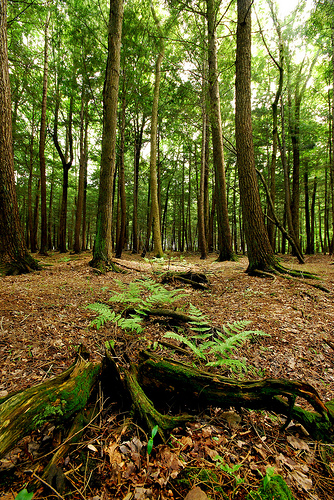
\includegraphics[width=0.48\textwidth]{images/forest.jpg}
%    \vspace{-10pt}
%  \caption{\textit{North American Forest} \label{fig:forest}}
%\end{wrapfigure}
\subsection*{Forest Characteristics}\label{subsec:forestcharacteristics}
Many different types of forest can be found in the Hudson Valley Region.
Because our region is an important biome transitional zone between the
oak-hickory, northern hardwood, and boreal forest types, we have nearly ten
boreal and more than twenty southern temperate tree species living near or at a
range limit ~\citep{ldeo}. This means that we have more species of trees than other regions
further to the north or south, and this forest biodiversity in turn supports
many important and iconic wildlife species such as black bear, wild turkey, and
numerous migratory song birds. These species are dependent on healthy, intact
forest patches to maintain their populations.
\par
To better quantify the ecological and commercial value of forested land, it is
important to designate its significance within the region.
\begin{itemize}
    \item \textit{Regionally significant forests} contribute to resiliency in a
        changing climate and have a high conservation value because of that
        function. Preserving these larger blocks of forest and the linkage zones that
        connect them will maintain wildlife corridors, reduce the impact of invasive
        species, and provide recreational benefits to areas experiencing growth in
        eco\-tourism. 
    \item \textit{Locally significant forest} blocks are equally important to regulating temperature and controlling the effects of whether
        events, but often have reduced habitat value for wildlife. Areas where
        development has infringed on forest habitat often see a more limited
        capacity for forest regeneration due to a higher presence of invasive
        species and over browsing by deer among other factors.  
    \item \textit{stepping stone forest} is important because it provides a
        bridge between these larger patches of biodiverse forest and allows
        for the establishment of ecological networks or corridors that help
        lessen the fragmentation of forest habitat, maintain the integrity
        of migratory pathways, and generally increase the viability of
        plant and animal wildlife.
\end{itemize}

\subsection*{Forest Patches and Regional Linkage Zones Map}
\label{subsec:forestpatchesandreglinkagezonesmap}
Because certain portions of Cornwall lie within the boundaries of two state
parks and the Black Rock Forest Consortium, our municipality’s overall forest
cover is considerable compared to others. This map shows the forest cover
within the borders of Black Rock Forest and on the adjacent land of West Point
to the south as regionally significant both for its size and the wildlife
habitat that it supports.
\par
Much of the village is classified as locally significant forest despite its
low-density residential development, and plays an important role in linking the
regionally significant forest patches to the river as well as providing a
buffer zone from more robust human development. The land protected by
Schunnemunk State Park is similarly classified as being locally significant and
is a reflection of the fact that continued development threatens to create a
habitat island, isolated from more biodiverse forest land.
\par
Outside of these areas, the map identifies large parts Cornwall as containing
stepping stone forest cover. The map also shows that most of these stepping
stone forest areas act as important regional linkage zones between locally and
regionally significant forest patches, and even combine with the regionally
significant forest of the Hudson Highlands to define the area between County
Rt. 32 and the southeastern border of the town as vital matrix forest (see
below). Of particular note in these stepping stone forest designations are
parts of Cornwall such as the land adjacent to state Rt. 9W and the Moodna
Creek that have been proposed for large scale residential development in the
past.
\includepdf[pages=-,fitpaper]{cornwall_maps/ForestPatchesRegionalForestLinkageZones.pdf}
\label{map:forestpatches}

\section{Stream and Riparian Habitat}\label{subsec:streamandriparianhabitat}
\subsection*{Why you need this map}
We all have enjoyed, been impacted by, or taken actions that impact Cornwall's
stream and riparian habitats. Cornwall Elementary School at Lee Road students
learn about the riparian habitat of Black Rock Forest reservoirs during their
3-season scientific expeditions. Parents and grandparents enjoy teaching their
children and grandchildren how to fish at Ring’s Pond. Some children will
disappear for hours along our many streams, exploring the plants and animals
that call these habitats their home and cooling off on hot summer days. As the
frequency of heavy rainstorm has increased by 74\% since the 1950s, we have
also experienced the swelling of our streams beyond their channels to former
floodplains where we have built many of our homes and other structures. We may
have inadvertently exacerbated this situation by removing the vegetation that
not only protects the plants and wildlife in our watercourses, but also
protects our properties from these floodwaters.
\par
Streams and streamside, or riparian, areas are important transitional zones
where land and water are linked ~\citep{haeckel2014}. Streams include the banks,
floodplains, and non-floodplain areas next to streams. Streams, if healthy, can
support the plants and microhabitats of small aquatic animals that are
important to the survival of native fish, like brook trout, American eel, and
herring species. Additionally, streams are key in the life cycles many other
species, like mink, bats, belted kingfisher, herons, wood turtles, stream
salamanders, and dragon flies by providing food and areas for breeding,
migration, hibernation, and safety. ~\ref{app:cornwall_species}
provides a comprehensive listing of species of conservation concern. Retaining
current floodplains supports habitats that can withstand occasional flooding,
such as meadows, swamp, marsh, and lowland forest, thereby supporting the
animals that rely on these habitats and other animals that rely on them for
food ~\citep{haeckel2014}.
\par
Maintaining the health of stream and riparian habitats involves the retention
and addition of native trees for shading to keep streams cool for our coldwater
fish, brook trout. The retention and addition of native shrubs, grasses, and
wildflowers can protect animal life by preventing unwanted vegetation,
sedimentation, and pollution reaching our streams and waterbodies as well as
reduce the impact of flooding. Orange County Water Authority's
\href{https://www.orangecountygov.com/DocumentCenter/View/4135/Watershed-Design-Guide-2014-PDF}
{Watershed Design Guide} provides a comprehensive visual explanation of healthy
streamside plantings based on the recommendations detailed in its
\href{https://www.orangecountygov.com/DocumentCenter/View/4133/Moodna-Creek-Watershed-Conservation-and-Management-Plan-2010-PDF}{Moodna
Creek Watershed Conservation and Management Plan} The Upper Esopus Creek
Management Plan Newsletter of Cornell University Cooperative Extension Ulster
County provides sample native streamside plantings for our neighbor to the
north, Ulster County.

\subsection*{Town of Cornwall and Village of Cornwall-on-Hudson}
\subsection*{Stream Classification Map}
%(hyperlink to that section in the narrative)
This map informs us of the existing or best uses of our local streams as well
as their quality and purity. According to the 2017 \gls{nysdec} data, many
streams in the Town are suitable trout habitat, with some suitable for trout
spawning, or release of eggs.

\subsection*{Stream Biomonitoring and Priority Waterbodies Map}
Notable on this map are the many dams and culverts that pepper our streams.
Culverts, if properly installed, can foster the natural life cycles of trout
and American eel, for example, by allowing them to travel upstream. While
long-standing dams have created much-appreciated features such as lakes and
ponds, it is now understood that they also play a role in isolating and
severely limiting the range of aquatic species and other organisms that use
stream corridors as well as a role in increasing local flooding and
deteriorating water quality ~\citep{haeckel2014}.
%(hyperlink to that section in the narrative)
%Good location for image of culvert 

\section{Wetland Habitat}
\subsection*{Why you need this map}
Wetland habitats serve two very important roles: they are key to the survival
of many species while providing flood-control and water cleansing benefits for
Town and Village communities. Wetland habitats come in many different forms and
support many different types of species. They include wet clay meadows,
hardwood swamps, emergent marches, and vernal pools. According to
\gls{nysdec}'s 
~\ref{app:cornwall_species}, our wetlands are home to the following
animals and plants that are threatened, of special concern, or of greatest
conservation need: Least Bittern, Common Snapping Turtle, Northern Copperhead,
Marbled Salamander, Clustered Sedge, and Large Twayblade.
\href{https://ecode360.com/10555547?highlight=wetlands#10555547}{Chapter 90
Freshwater Wetlands} of the Town’s Code provides a comprehensive listing of the
vegetation that is associated with seasonal or permanently flooded wetlands.
Beavers, muskrats, and dragon flies are just a few of the additional animals
for which wetlands are important.
\par
Vernal pools are of particular interest because they are typically small in
size and not well documented. These seasonal woodland pools don't always
support wetland vegetation, but they are critical breeding habitat for several
species of forest salamanders and frogs, such as spring peepers
~\citep{haeckel2014}. A wetland ground-truthing exercise would be instrumental
to identifying not only seasonal wetlands, but also smaller wetland habitats
that are not captured by the various data sources for the 
~\nameref{map:wetlandsandhydricsoils}. See section ~\nameref{subsec:wetland}
for more information.

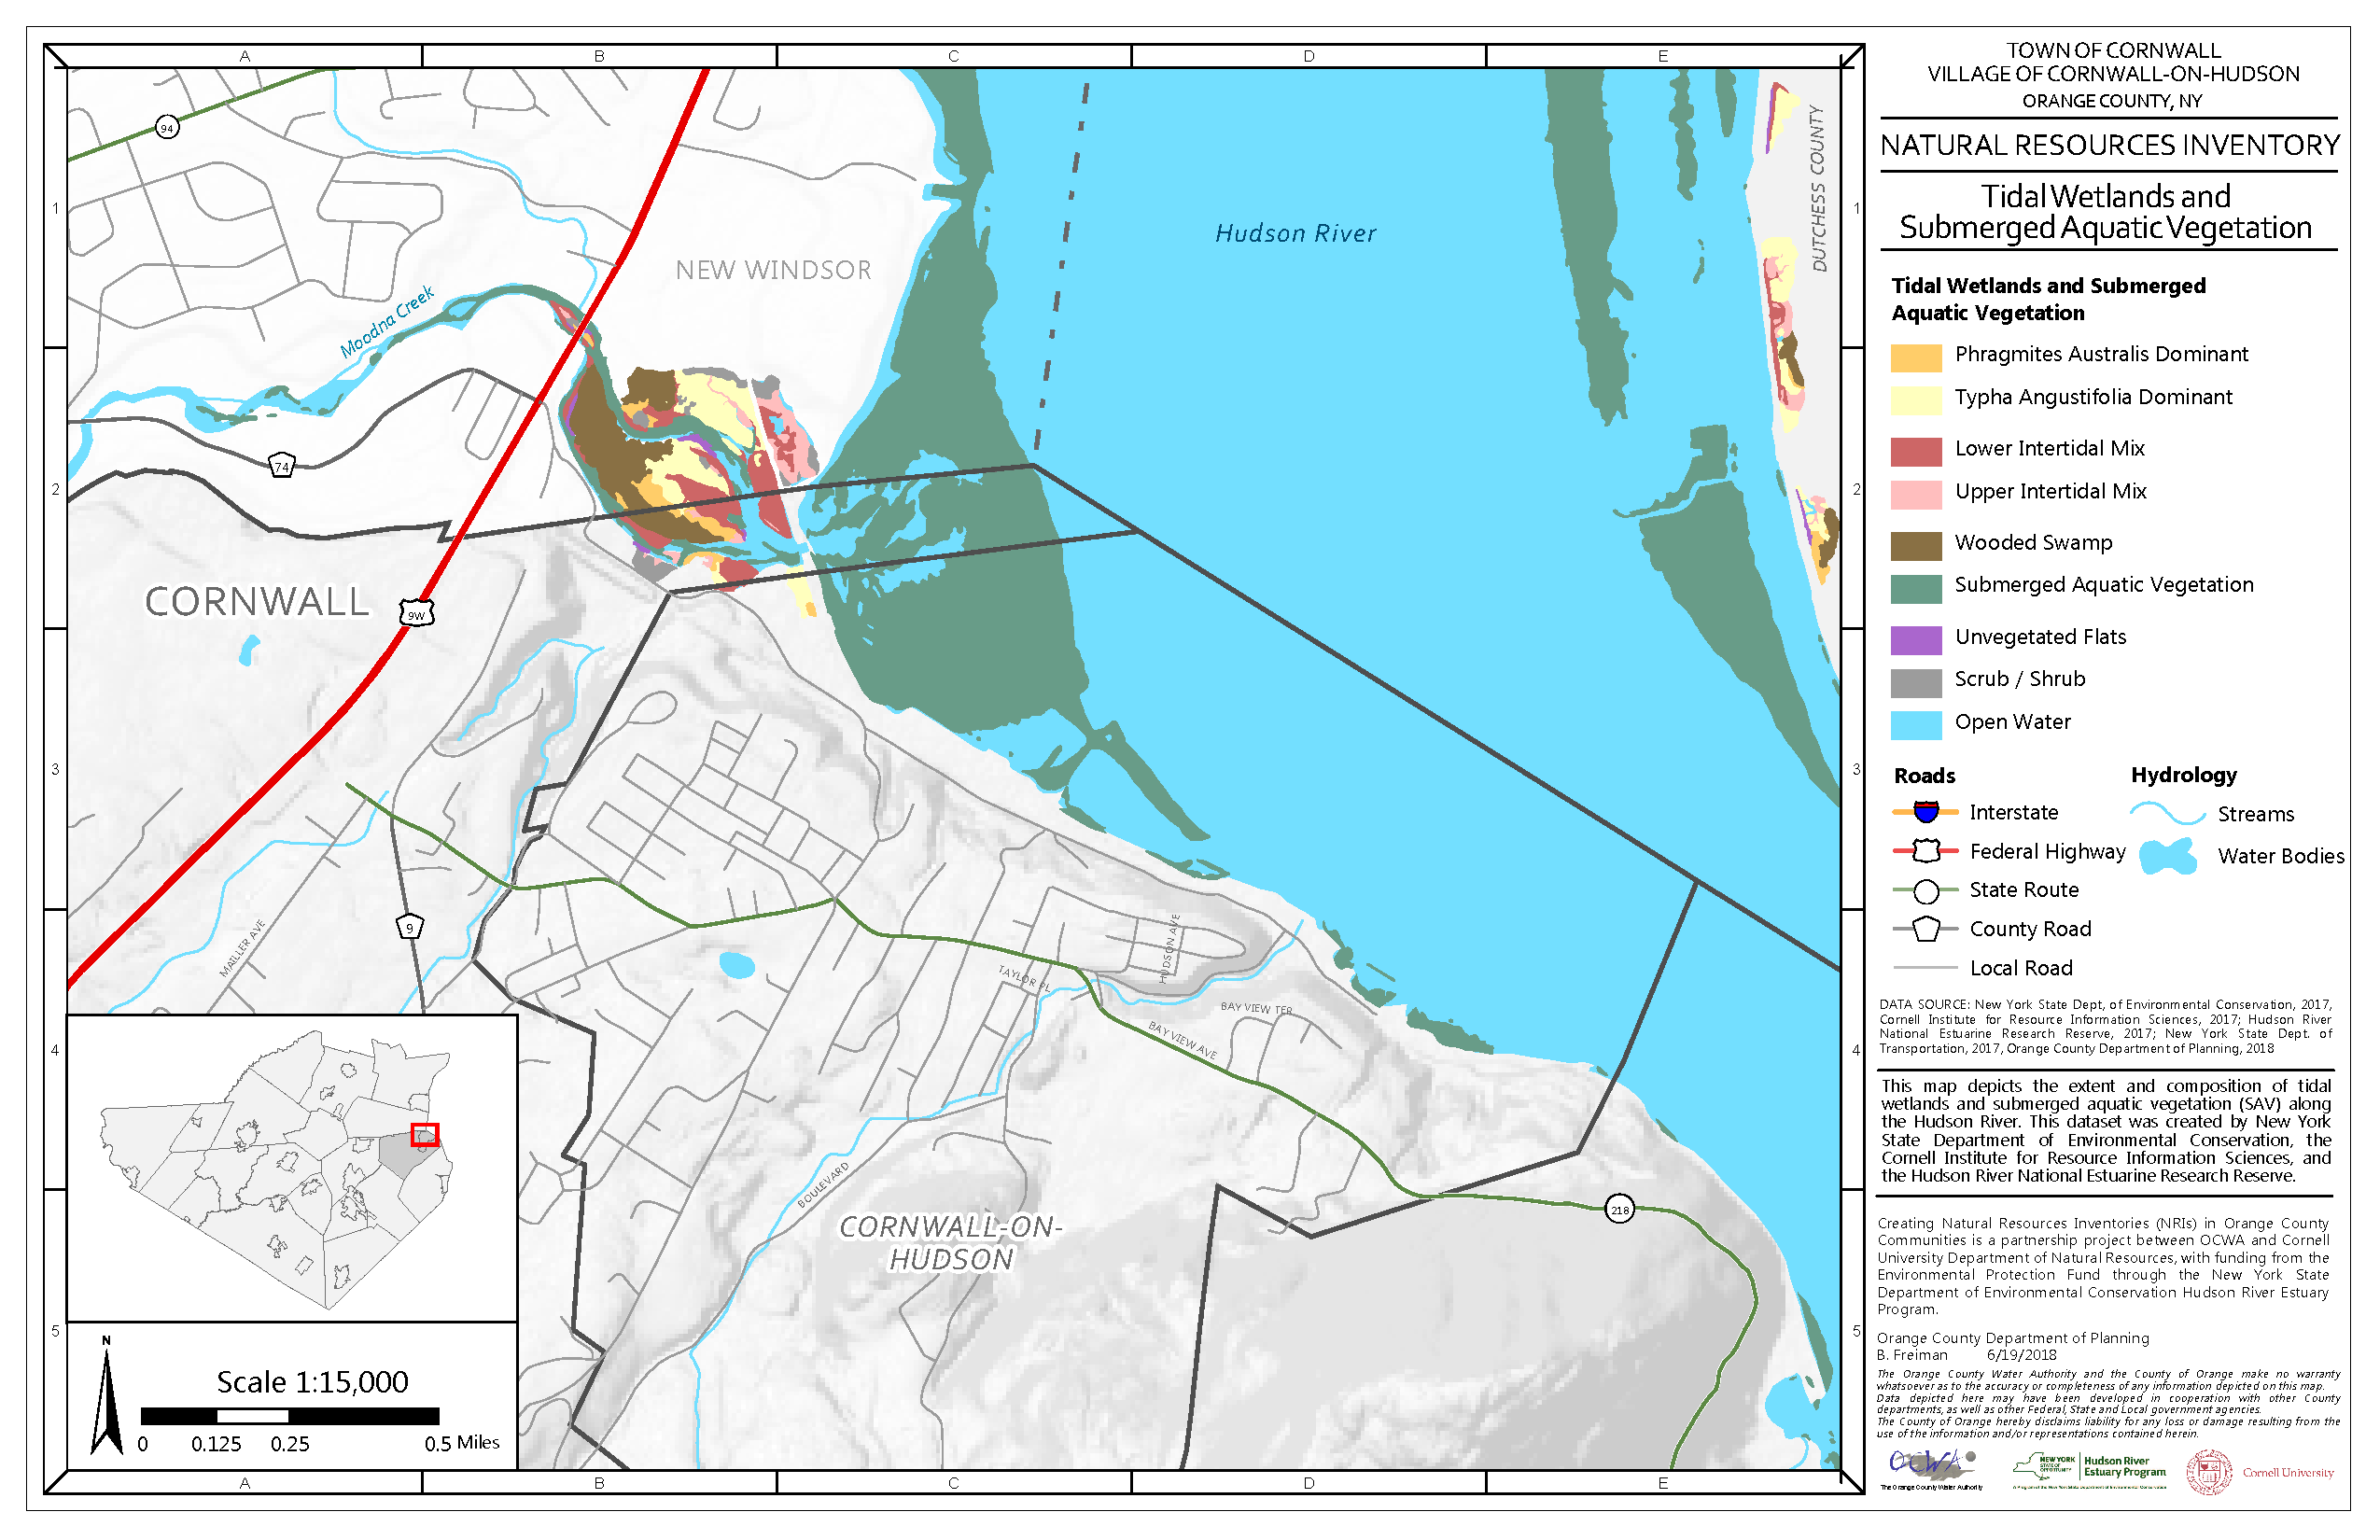
\includepdf[pages=-,fitpaper]{cornwall_maps/TidalWetlandsandSAV.pdf}\label{map:tidalwetlandsandSAV}
\section{Tidal Wetland Habitat}\label{subsec:tidalandwetlandhabitat}
Tidal wetlands are some of the most important habitats within the Hudson River
Estuary. They support numerous unique species that rely on the changing water
level to survive, and that are especially suited for that habitat type. Tidal
wetlands and \gls{sav} not only support a great diversity of plant, animal, and
insect life, they also contribute to the economic significance of the estuary.

\begin{displayquote}
More than 200 species of fish are found in the Hudson, including key commercial
    and recreational species like striped bass, and species of conservation
    concern like Atlantic and short-nose sturgeon. \gls{sav} beds improve water
    quality in the Hudson and provide essential habitat for invertebrate
    animals, which feed fish and waterfowl that use the estuary. Tidal wetland
    habitats play a critical role as nursery grounds for fish and shellfish
    species, as well as providing nesting sites and migration stops for birds
    and sources of nutrients for the estuary food web. These wetland systems
    also help filter pollutants, buffer shoreline properties, and help
    stabilize the river’s shoreline ~\cite{haeckel2014}.
\end{displayquote}

Given the trend of sea level rise due to climate change, \textbf{it is also
important to note that tidal wetlands can help reduce flooding by limiting wave
action and acting as an intermediate habitat between the land and the water.}
They are often great places for recreation, providing opportunities for fishing
exploring by kayak or canoe. 
\begin{wrapfigure}{r}{0.5\textwidth}
    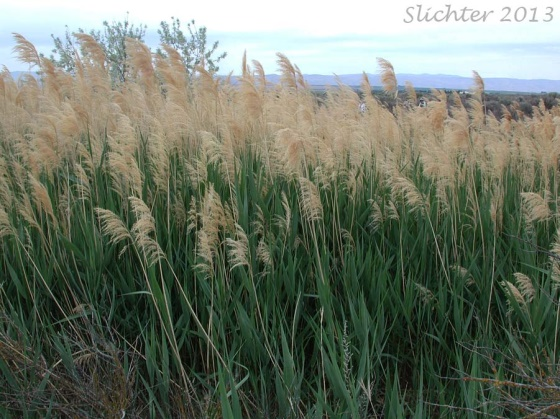
\includegraphics[width=0.48\textwidth]{images/Common_reed.jpg}
  \caption{\textit{Phragmites australis}}
\end{wrapfigure}

Since tidal wetlands are extremely dynamic systems, they are constantly
changing. However, long term changes can be seen in vegetation type and
sediment levels. Many wetlands have been invaded by the common reed
(\textit{Phragmites australis}). Areas with native cattail (\textit{Typha
angustifolia}) tend to be much more biologically diverse than areas invaded by
Phragmites, and more biodiversity in the plant community can increase the types
of other animals that use a given area for shelter or food. As the climate
changes and sea level rises, water levels may increase faster than wetlands can
gain new sediment, which could cause decreased amounts of these crucial
habitats for plants and animals ~\citep{nysdectidal}. 
\par
\gls{sav} provides important habitat for juvenile fish that can hide within the
leaves. In addition to fish, \gls{sav} beds provide habitat for
macroinvertebrates, and food for waterfowl, either by eating the plants
themselves or eating the animals living in the plant beds. \textbf{\gls{sav} is
an important source of oxygen in the water, which aquatic animals need to
survive and is used as a key measure of water quality.} Water celery is the
most common native submerged aquatic plant in the Hudson River. A very common
invasive species impacting \gls{sav} is water chestnut (\textit{Trapa natans}),
which can be seen in almost every freshwater, slow moving area of the Hudson
River in the summertime. Water chestnut creates mats of leaves at the surface
of the water, shading out native water celery below. The water underneath water
chestnut beds are known to have much lower oxygen levels than other areas.
While water chestnut does produce oxygen, they release it into the air through
their leaves floating at the top of the water, instead of directly into the
water like other aquatic plants would ~\citep{nysdecsav}.

\vspace{3mm}
\begin{wrapfigure}{l}{0.5\textwidth}
    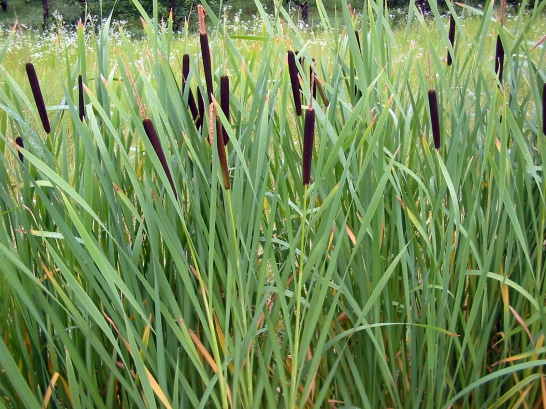
\includegraphics[width=0.48\textwidth]{images/Cattail.jpg}
  \caption{\textit{Typha angustifolia}}
\end{wrapfigure}

\textbf{Although these habitats support extraordinary biological diversity and
provide important benefits to humans, they have been diminished, damaged and
disconnected by human patterns of development during the last 150 years.} Vast
areas of river bottom have been dredged to create and maintain a shipping
channel. Tidal wetlands and shallows have been filled, and, in some areas, fill
covers a third of the river's original surface area. Nearly half the Hudson's
shoreline has been straightened and hardened by human-made structures.
Compounding these losses are impacts from sea-level rise and climate change
which threaten shoreline and shore communities where water may rise faster than
habitats can build up sediments to keep pace. Also, human responses to
sea-level rise and increased flooding may include building dikes which will
prevent habitats from migrating landward. Finally, the ongoing accidental and
deliberate introduction of invasive plants and animals continues to threaten
native species and their habitats ~\citep{nysdosmoodna, anderson2013}.

\begin{wrapfigure}{r}{0.5\textwidth}
    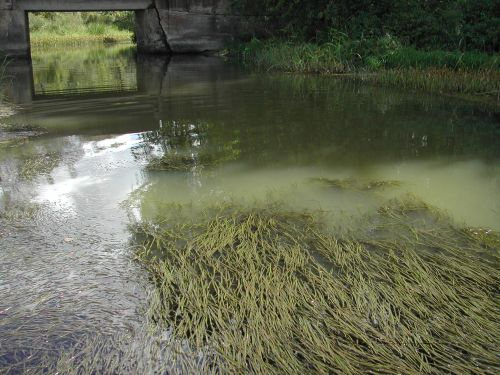
\includegraphics[width=0.48\textwidth]{images/Water_Celery.jpg}
  \caption{\textit{Vallisneria americana}}
\end{wrapfigure}

\subsection*{Tidal Wetland Habitat}
Cornwall has only a small area of tidal wetlands, but that area, the mouth of
the Moodna Creek, is an important component in Cornwall’s contribution to the
overall health of the Hudson River estuary. The map shows the distribution of
the two primary tidal wetlands reed species common to the area, \textit{Typha
angustifolia} (native) in yellow and Phragmites australis (invasive) in orange.
Also shown are wooded areas (brown), barren areas and mud flats (purple), and
areas of upper and lower intertidal mixed vegetation (pink and red,
respectively).
\par
To the east of the Moodna outlet is a large area of submerged aquatic vegetation 
(dark green). This \gls{sav} growth follows along much of the shore line of the 
town and village with the exception locations where development has occurred and 
hardened shoreline has been created (i.e.; Donahue Park). Submerged aquatic 
vegetation is also present through most of the Moodna creek outlet and runs 
approximately 2/3 of a mile up the creek itself in patches. All of this 
\gls{sav} provides important nursery habitat for numerous fish and wildlife 
species.

\section{Grasslands and Shrublands}\label{subsec:grasslandsandshrublands}
\subsection*{Why this habitat is important}
\begin{wrapfigure}{l}{0.5\textwidth}
    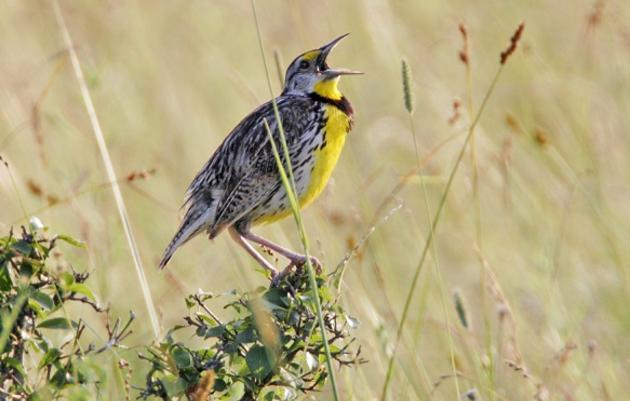
\includegraphics[width=0.48\textwidth]{images/bird.jpg}
  \caption{A bird}
\end{wrapfigure}
Meadows, grasslands, and shrublands are unique and valuable habitats that are 
critical for bird, plant, and wildlife communities. Historically, Native 
peoples, fires, and beaver were the primary forces responsible for creating and 
maintaining grassland and meadow habitats in New York. Native Americans created 
grasslands when they burned the land for agriculture and to improve forage for 
game species such as white-tailed deer. At the same time, ponds above abandoned 
beaver dams grew into grassy meadows after the water drained and the 
nutrient-rich soil was exposed to sunlight. In more recent history, fire 
suppression and limits to where beavers are allowed to build dams has meant that 
grass and shrublands are restricted mainly to agricultural areas. The peak of 
agricultural clearing in the northeastern US occurred in the mid-1800s 
~\citep{unhextension} Since then, \textbf{the amount of land identified as grassland or 
shrubland has decreased rapidly in the Northeastern United States}. This is 
mostly due to increases in population and resulting development, and changes in 
agriculture that has resulted in the abandonment of many small, family-owned 
farms. Unused farm land has traditionally been a major target for sale and 
development and is typically one of the first habitats to succumb to low-density 
residential development.
\par
Native wildflower growth in these habitats is a vital source of support to
pollinators, and numerous species depend on open grassland and shrubland
habitats, especially grassland breeding birds that require large meadows for
successful nesting. New York State's grasslands are home to significant
populations of some of the highest priority birds in the Atlantic Flyway. These
birds, which have been sentinels of environmental health for centuries, depend
on hayfields, pastures, fallow fields, and other agricultural lands for
essential habitat. But the same bird species are experiencing significant
declines in populations. Scientists report a 90\% decrease in targeted
grassland species since 1966 ~\citep{audoboniba}. Some of these species such as Henslow's
Sparrow, Upland Sandpiper, Grasshopper Sparrow, Short-eared Owl, and Eastern
Meadowlark are area-dependent species, meaning that they need large unbroken
expanses of grasslands to thrive and reproduce. The amount of grassland habitat
needed by these species depends on factors such as location, shape, surrounding
habitats, and vegetative composition, however, as a general rule, grasslands
need to be at least twenty-five acres in size to offer appropriate habitat for
at-risk grassland birds in New York. The ~\ref{map:areasofknownimportance}
map shows the extent of the Audubon Important Bird Areas that lie within the
borders of Cornwall.
\par
Old farm fields or forest clearings are by nature transitional and relatively
short-lived habitats, usually quickly colonized by shrubs and requiring
periodic management to maintain openness. Shrublands in turn revert rapidly to
forest without continued maintenance or disturbance, such as fire, that
triggers young forest growth. Where they still occur, conserving and managing
large grasslands and shrublands benefits wildlife and can also support
agricultural land uses and scenic values ~\citep{haeckel2014}.
\subsection*{Meadows, Grasslands, and Shrubland Map}
Cornwall is home to a considerable amount of meadow, grassland and shrubland.
Much of the town’s land that is not mountainous or developed falls into this
category. This map shows all of the significant parcels within the Town of
Cornwall and the Village of Cornwall-on-Hudson Cornwall ranked by acreage; the
lightest shading being small parcels of 10 or fewer acres, and the darker
shading denoting large parcels of more than 50 acres. Most of Cornwall's large
parcels of grasslands and shrublands are located in the west of the town,
clustered at the foot of Schunnemunk Mountain. Other significant parcels lie on
either side of State Route 94 and County Route 20 (Orrs Mills Road).
\par
Cross referencing the ~\nameref{map:landcover} under the land use section in
this NRI shows that the majority of these grasslands and shrublands are either
actively cultivated farmland or pasture, or preserved lands that were
previously cultivated and left as pasture. Looking at the ~\ref{map:protectedopenspace}
map in the land use section, one can see that significant portions
of these preserved grasslands and pasture are now within the boundaries of
state parks, public nature preserves, museums, or conservation easements.
Because these lands are preserved and actively maintained, this ensures that
annual mowing occurs and keeps these parcels from becoming shrubland and
returning back to forested land. As noted above, this is important for
maintaining vital grassland bird habitat in the Hudson Valley.
\par
While the Village of Cornwall-on-Hudson is heavily forested outside of its
central developed areas to the north, it does contain a number of grassland
parcels, the most significant being the former Donahue Farm parcel off of
Hudson Street. Privately owned and maintained land accounts for the other
significant grassland or shrubland parcels in the Village.
% 218?
\includepdf[pages=-,fitpaper]{cornwall_maps/MeadowsGrasslandsandShrublands.pdf}
~\label{map:meadowgrasslandsandshrublands}

%***************Water Resources******************
\part{Water Resources}\label{sec:water}
\chapter{Watersheds}\label{subsec:watersheds}
\subsection*{Why you need this map}
When we view our communities using satellite imagery, we see the developed 
areas, green space in the form of woodlands, farmland, meadows, and water 
bodies, such as streams, river, lakes, and wetlands. In a two-dimensional 
viewing, it is difficult to visualize the direction in which these waterbodies 
naturally flow. A watershed map serves the purpose of identifying the direction 
in which all surface waters flow within a specific land area to a waterbody. 
Highpoints, such as ridges, mountains, and hills, form the typical dividing 
lines of watersheds and represent the point from which all water flows 
downward. Watersheds may be further divided into the smaller drainage areas, 
known as subwatersheds or sub-basins. Because watersheds do not follow 
municipal boundaries, working in a watershed context requires communication and 
coordination between multiple municipalities. Maintaining healthy watersheds is 
important because watersheds provide critical natural services that sustain and 
enrich our daily lives, such as plentiful and safe drinking water.

\begin{wrapfigure}{l}{0.5\textwidth}
  \centering
    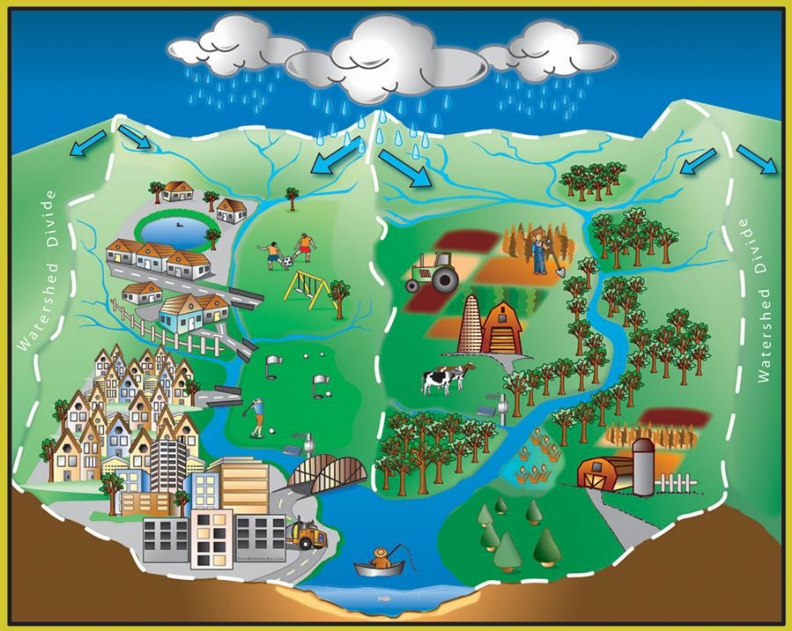
\includegraphics[width=0.45\textwidth]{images/watershed_riveralliance.jpg}
  \caption{Watershed diagram}\label{fig:watershed}
  \vspace{-20pt}
\end{wrapfigure}

What are other critical natural services that healthy watersheds can provide? 
They reduce erosion and provide critical habitat for plants and animals. They 
are areas of natural beauty that can offer wonderful opportunities for 
recreation and relaxation, like local streams and lakes. They are important 
features of our local geography and rural character. Lastly, healthy watershed 
can "minimize public infrastructure and water treatment costs and help increase 
our resilience to extreme weather events" by storing floodwaters in intact 
flood plains and riparian areas ~\citep{haeckel2014}. 
\href{
https://www.epa.gov/sites/production/files/2015-10/documents/economic\_benefits\_f
actsheet3.pdf}{The Economic Benefits of Protecting Healthy Watersheds 
Factsheet} highlights economic benefits, such as New York City’s 80\% cost 
savings from watershed conservation efforts when compared with the construction 
of new water filtration plants ~\citep{usepa2012}.
\par
This watershed diagram from the \href{https://thewhiteriveralliance.org/}{White 
River Alliance} depicts the various developed features water may encounter on 
its way to a local waterbody, such as farmland, residential areas, industry, 
commercial areas, and transportation infrastructure. Local policies can 
dramatically impact a municipality's water availability and quality. For 
example, does local zoning allow for structures to be constructed too closely to 
streams and wetlands, or are ample buffer zones incorporated into the zoning 
code? Is a municipality considering limiting further development on remaining 
floodplains to protect existing and future construction from floodwaters and 
heavy storms? Collaboration with neighboring municipalities can be critical to 
fostering healthy watersheds and maintaining plentiful water in a local 
jurisdiction. Is there intermunicipal collaboration around the development of 
policies that can benefit many municipalities within a watershed? Watershed 
councils, such as the 
\href{http://waterauthority.orangecountygov.com/moodna\_council.html}{Moodna 
Creek Intermunicipal Watershed Council}, can play an important role in these 
intermunicipal collaborations in partnership with local water authorities, like 
the \href{http://waterauthority.orangecountygov.com/index.html}{Orange County 
Water Authority}.
\subsection*{Watersheds and Sub-basins Map}
Orange County municipalities lie within 10 watersheds, as is shown on an inset 
map of the Town of Cornwall and Village of Cornwall-on-Hudson Watersheds and 
Sub-basins map.

The Town lies primarily in the Moodna Creek Watershed. All of the waterbodies 
within this watershed drain to the mouth the Moodna, which straddles the towns 
of Cornwall and New Windsor along the Hudson River Estuary just north of the 
Village (D1). Two small portions of the Town fall within the Lower Hudson 
Watershed.
\begin{itemize}
  \item The Moodna Creek Watershed within the Town's boundaries includes two 
    sub-basins, the Woodbury Creek Sub-basin (darker green) and the 
    Silver Stream-Moodna Creek Sub-basin (lighter green).
  \item The waterbodies in the Woodbury Creek Sub-basin flow into Woodbury 
    Creek. This includes Mineral Spring Brook, with headwater at Sutherland 
    Pond, and Woodbury Creek itself, which then joins Moodna Creek at B3.
  \item The waterbodies of the Silver Stream-Moodna Creek Sub-basin flow 
    into Moodna Creek by way of Silver Stream in New Windsor and Idlewild 
    Creek, with tributary sources in Sphagnum Pond, Arthur’s Pond, Aleck Meadow 
    Reservoir, and Upper Reservoir. These waterbodies are all located within 
    Black Rock Forest.
  \item The Lower Hudson Watershed portions within the Town's boundaries 
    includes the Breakneck Brook-Hudson River Sub-basin (brown) and the 
    Popolopen Creek Sub-basin (dark pink), which flow to the Hudson River.
\end{itemize}
The Village lies almost entirely in the Lower Hudson Watershed (brown). All 
waterbodies flow directly into the Hudson River, including the streams off Deer 
Hill and Storm King Mountain.

All waterbodies within the Town’s and Village’s watersheds flow through 
developed residential and commercial areas, roadways, and pristine forest.

\includepdf[pages=-,fitpaper]{cornwall_maps/WatershedsandSub-basins.pdf}\label{map:watershedsandsubbasins}

\chapter{Groundwater and Aquifers}\label{subsec:groundwater}
\subsection*{Why you need this map}
The Watersheds and Sub-basins section (hyperlink to section) discussed the 
water that flows over land and how it interacts with existing land uses, 
impacting water quality in our waterbodies. The policies and practices that a 
municipality may have in place to protect the health of our waterbodies also 
protect the health of groundwater. Additional protective measures are also 
needed to protect the health of groundwater as groundwater supports not only 
habitats and their species but also our drinking water.

\subsection*{Aquifers}\label{subsec:aquifers}
This \href{http://rdnwaterbudget.ca/water-101/aquifers-groundwater/}{image}
from the Regional District of Nanaimo in British Columbia 
illustrates the interactions between precipitation, surface water, and 
groundwater. Precipitation can go directly to a waterbody, like a stream or 
pond, or it can infiltrate into soil and move into rocks through cracks and 
pores. The water in the unsaturated zone lies above the water table; it is 
closely mixed with grains of gravel, sand, silt, and clay, and hydrates plants 
and soil-dependent creatures.
\par
\begin{wrapfigure}{l}{0.5\textwidth}
    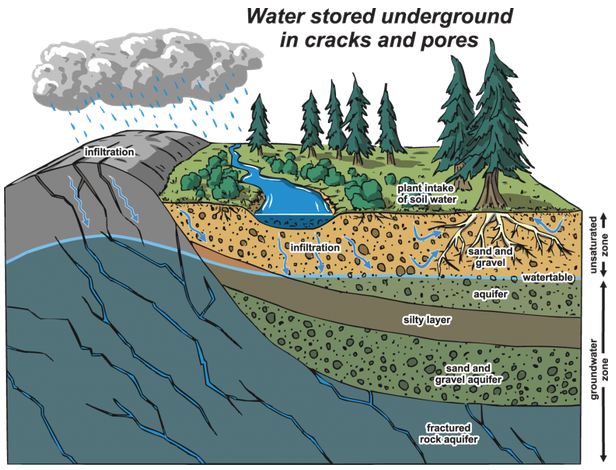
\includegraphics[width=0.48\textwidth]{images/aquifers.png}
    \vspace{-10pt}
    \caption{Water cycle}
    \vspace{-10pt}
\end{wrapfigure}
Aquifers lie in the saturated zone below the water table and are the source of 
our drinking water. They are the ``zones in sediments and bedrock that 
receive, store, and transmit significant amounts of water to wells and 
springs``~\citep{haeckel2014}. The area of land that contributes to recharging 
aquifers is called the aquifer recharge area; this area can be as large as an 
entire watershed or a sub-basin. Aquifers also have discharge areas, which feed 
perennial streams, linked ponds/lakes, and riparian wetlands.
\par
With more than 25\% of New Yorkers dependent on groundwater for drinking, 
municipalities have an important role to play in ensuring that drinking water 
remains plentiful and clean. While regional aquifer depletion in New York is 
rare, thanks to our plentiful precipitation, localized depletion can occur when 
withdrawals exceed natural local recharge rates. Municipalities can implement 
protective measures to support a balance between withdrawals and natural 
recharge, thereby protecting wells and the waterbodies that depend on 
groundwater. Municipalities can also foster an awareness of aquifer pollution 
and enact preventive legislation. These efforts can focus on the various sources 
of aquifer pollution: chemical spills; run-off of oil, gas, and antifreeze from 
motor vehicles; road salt; common household cleaners, herbicides, and 
pesticides; underground storage tanks; and improperly spaced or faulty septic 
systems and improperly maintained public sewer systems. An important first step 
can be the development of a management plan for the protection of groundwater; 
the New York Rural Water Association offers technical assistance for the 
development of \href{ 
http://www.nyruralwater.org/sites/default/files/Fact\%20Sheet10\_1-5-2018.pdf}{ 
source water protection plans}.

\subsection*{Public Wells, Aquifers, and Risk Sites Map}
Cornwall is fortunate to be underlain by many below water table aquifers, 
depicted as the pink, green, and brown areas on the map. The Town and Village 
also have four sizable above water table aquifers, appearing as yellow on the 
map. They are located primarily along the Moodna Creek, Woodbury Creek, and on 
the banks of the Hudson River. Orange County Water Authority's 
\href{
http://www.kj-seqra.com/507Acres/ReferenceMaterial/OCWA\%202008\%20Moodna\%20Wat
ershed\%20Atlas\%20(39MB).pdf}{Moodna Creek Watershed Atlas} classified all of 
Cornwall’s aquifers as "Important Groundwater Sources" and, as such, are 
important to drinking water.

\includepdf[pages=-,fitpaper]{cornwall_maps/WellsandRiskSites.pdf}
\label{map:wells}
\namedlabel{map:wellsandrisksites}{Public Wells, Aquifers and Risk Sites Map}

\subsection*{Wells}\label{subsec:wells}
Cornwall has four sources of drinking water: local surface water from the 
Village of Cornwall-on-Hudson’s reservoirs in Black Rock Forest, surface water 
from New York City’s Catskill Reservoir System via the Catskill Aqueduct, 
private wells, and public wells. This diversity of water sources provides great 
flexibility to provide uninterrupted, high quality drinking water to the Town’s 
residents. It is our most precious natural resource.

Cornwall's public wells are indicated by blue dots on this map, with many lying 
directly over aquifers. They are located along Taylor Road, near the Moodna 
Creek (B3). The map also seems to indicate the presence of two additional wells 
along Angola Road just southwest of Route 9W and near the intersection of Angola 
Road and Mineral Springs Road; however, the Village Water Department has no 
knowledge of wells at that site. The drilling of new wells must be carefully 
monitored for negative effects on surrounding public and private wells. 
Excessive extraction can change stream flow and water temperature, affecting the 
survival and reproduction of aquatic life.

\subsection*{Risk Sites}\label{subsec:risksites}
The map also shows many risk sites. These include petroleum bulk storage 
facilities (brown dots) and remediation sites (pink diagonal lines), many of 
which are located directly over or adjacent to aquifers. There is only one 
chemical bulk storage facility of record located near the aquifer that 
underlays the Cornwall Town Landfill (C2). Removing these bulk storage 
facilities from these sensitive locations should be explored; change in property 
ownership may present opportune times for removal.

The map shows four NYSDEC remediation sites. They include:
\begin{itemize}
    \item The Star Expansion site on Industry Drive in Mountainville, between 
    the NYS Thruway and Woodbury Creek (B4). The Groundwater on-site is 
    contaminated with chlorinate solvents. Public water supply wells are 
    located within 1000 meters of the site, but are hydrogeological 
    upgradient, meaning that any onsite contaminants cannot flow 
    uphill. Private residential wells are located within 200 meters 
    and have shown no contamination. The site presents a significant 
    environmental threat due to the ongoing releases of contaminants from the 
    source areas into the groundwater/soil vapor.
    \item The Majestic Weaving Corporation site, on Mill Street, along the 
    Moodna Creek (C2). Remedial measures taken have removed contamination from 
    the site, therefore exposures to site contaminations are not expected.
    \item The inactive Cornwall Town Landfill site located between the NYS 
    Thruway and Route 32 on Halloran Road on the north side of the Town (C2). 
    The municipal waste landfill was closed in 1977. The site is currently 
    being used for leaf composting and storage of gravel. Nearby wells have 
    been sampled by the Department of Health. No contaminants were found.
    \item The area at the southern tip of the Town, shared by the Towns of 
    Woodbury and Highlands and the location of many unexploded ordinances.
\end{itemize}
% link to GPS coordinates or parcel reference?
The map also shows three \gls{spdes} permitted 
locations (purple diamonds): Star Mountainville Industrial Park (B4) 
discharging into Woodbury Creek and discharges from sewage treatment plants into 
Moodna Creek at C2 and at the mouth of the Moodna (D1). SPDES is a permit 
program that allows permitted businesses, municipalities, and individuals to 
dispose of wastewater under highly regulated conditions to prevent the pollution 
of local waterbodies Proper treatment of wastewater is important to reducing the 
negative impact on water resources.

\chapter{Floodplains}\label{subsec:floodzones}
\subsection*{Why you need this map}
The New York Climate Change Science Clearinghouse notes that the Northeast and 
New York State have seen a 71\% increase in heavy precipitation events that 
have resulted in major and costly flooding. Typically flooding happens in 
low-land areas that are naturally prone to flooding, known as floodplains. These 
areas are next to streams and other waterbodies that can become engorged and 
overflow during heavy rainfalls and snowfalls.
\par
Flood zones are delineated by the \gls{fema} and the US \gls{hud}. Delineated 
flood zones typically include historic floodplains and their floodways. Two 
flood zone categories are commonly used: 100-year and 500-year flood zones. 
Land areas and all structures lying within a 100-year flood zone have a 1\% 
chance of flooding every year; areas within a 500-year floodplain have 0.2\% 
chance of flooding annually. Due to the increased frequency and severity of 
heavy precipitation events, communities throughout the US have seen multiple 
100-year flood events happen in a given year and repeated, annual 500-year 
events. The City of Houston, Texas, for example, has seen three 500-year floods 
in as many years ~\citep{dara2017}.
\par
%% check this
Delineated flood zones, however, are not the only places where flooding can 
happen. Flooding can take place anywhere as a result of poorly designed or 
inadequate culverts and dams (see ~\nameref{subsec:floodzones} section for 
further information). Haeckel and Heady explain that "[d]ue to many variables, 
such as the often-unpredictable nature of floods, local drainage problems, and 
the variable intensity of land development in watersheds, some flood-prone 
areas may not appear on designated floodplain maps, and floodplain designations 
may change over time as more information becomes available." The increase in 
impervious surfaces, like roads, driveways, and buildings, prevent absorption 
of floodwaters and results in increased stormwater run-off into waterways. As 
floodwaters travel over various land uses, pollutants are collected and 
deposited in habitats, thereby degrading them.
\par
Planning around locally known flood-prone areas can help municipalities reduce 
the impact of floods on their communities. Cornwall, for example, has long been 
subject to flooding events that have eroded hillsides, damaged structures, and 
even caused dislocation from businesses and residences. Local governments can 
institute policies and practices that harness the benefits of floodplains, such 
as slowing and storing floodwaters and reducing downstream flood damage, 
through conservative buffering around know flood-prone areas. Other benefits of 
preserved floodplains include creating a natural safety zone for development 
and the damaging impacts of floods. By implementing relevant policies, 
municipalities would also be supporting the plants and animals that "tolerate 
occasional flooding and support the in-stream food web" ~\citep{haeckel2014}.

\subsection*{Flood Zones and Flooded Roads Map}
The most significant floodplain areas in Cornwall are located along the Moodna 
and Woodbury creeks, on the Hudson River shoreline, and along smaller streams 
in residential areas of the Town and Village (see D2). The waterbodies shown on 
the map (springs, lakes, streams) contribute to the Moodna Creek’s flow. The 
Moodna forms in the Town of Blooming Grove, flows through the Village of 
Washingtonville and the Town of Cornwall, ending its path through the Town of 
New Windsor into the Hudson River. It is the culmination of these water sources 
that can also lead to the flooding that has devastated portions of these 
municipalities.
\par
The Flood Zones and Flooded Roads map also shows roads that were closed and/or 
flooded during Hurricane Irene in 2011 (yellow) and the April 2007 spring 
northeaster (red). During these extreme weather events, many properties located 
near the mapped flood zones were flooded – even those that were not in 
delineated flood zones.
\begin{itemize}
    \item Hurricane Irene closed many roads, including all segments of the NYS 
        Thruway that passes through Cornwall, Otterkilll Road, portions of 
        Route 32, Quaker Avenue, Continental Road, Hasbrouck Avenue, 
        the Boulevard, and other smaller local roads.
    \item The April northeaster closed all of Route 9W in Cornwall, along with 
        portions of Otterkill Road and Taylor Road near the Moodna Creek in 
        the western part of the Town.
\end{itemize}
\includepdf[pages=-,fitpaper]{cornwall_maps/FloodZonesandFloodedRoads.pdf}\label{map:floodzonesandfloodedroads}

\chapter{Wetlands}\label{subsec:wetland}
Whether you know them as marshes, swamps, or bogs, the many benefits of 
wetlands to humans, animals, and plants are widely recognized through 
protective governmental legislation, by scientists, and by those who enjoy the 
recreational features supported by wetlands. Some of these benefits include:
\begin{itemize}
    \item Acting as a buffer to control flooding and reduce damage from storm 
    surge.
    \item Serving as naturally-occurring filtration devices, cleansing surface 
    water of impurities.  Wetlands can remove or trap 20-60\% of metals, 80-90\% 
    of sediment, and 70-90\% of nitrogen (Ecological Society of America).
    \item Holding and slowly releasing water from sources like snowmelt, 
    rainfall, or runoff, thereby maintaining base streamflow and recharging 
    groundwater.
    \item Storing 1-1.5 million gallons of floodwater for every acre of wetland
    and supporting 75\% of commercially harvested fish through spawning areas 
    (US Environmental Protection Agency 2001).
    \item Producing food and organic material that supports commercial and 
    sport fisheries. Wetlands also provide "breeding, feeding, and wintering 
    habitat for hundreds of wildlife species," like birds, mammals, and 
    amphibians. (US Army Corps of Engineers 1998)
    \item Recreational activities, like kayaking, canoeing, birdwatching, 
    hunting, and fishing.
    \item Serving as natural "carbon sinks" by helping reduce atmospheric
    greenhouse gases through excess atmospheric carbon storage (Association 
    of State Wetlands Managers).
\end{itemize}

How do wetlands provide these important benefits? Wetlands are defined as "an 
area that is covered by shallow water or has waterlogged soils for long periods 
during the growing season in most years" (USACE 1998). Additionally, wetlands 
must have hydric soils and support "plants that require saturated soils to 
survive\ldots [or that] can tolerate prolonged wet soil conditions" (USACE 
Wetlands Identification). These features enable wetlands to act as, 
essentially, giant sponges. This image shows how wetland soils and their plants 
store water from both surface flow and groundwater flow, slowly releasing it to 
streams or aquifers.

Because of their critical ecological importance, wetlands are regulated by 
Section 404 of the Federal Clean Water Act and NYSDEC's Freshwater Wetlands 
Act. The presence of wetlands is often the reason many development projects are 
subjected to an environmental impact review under federal and/or state laws. The 
Freshwater Wetlands Act protects wetlands, and the 100-foot boundary around 
them, that are larger than 12.4 acres; smaller wetlands of unusual local 
importance are also protected. Many communities in NYS have recognized the 
importance of wetlands by enacting legislation that protects wetlands and vernal 
pools down to 1/10$^{th}$ of an acre through local wetland laws, wetland overlay 
districts, and supplemental zoning standards. The Hudson River Estuary 
Program/Cornell University created a very useful Summary of Municipal Wetland 
and Watercourse Protection Techniques, found in Appendix 
~\nameref{app:cornwall_wetlands}. These wetland protection techniques can address the 
impact that land use decisions can have on wetlands by considering adjacent 
upland areas and connected hydrologic features, like streams.

The sources of wetland data have limitations, requiring public information and 
on-site observations to identify smaller wetlands and confirm regulated wetland 
sized. Haeckel and Heady note that the Federally-designated US Fish and 
Wildlife Service’s National Wetland Inventory "maps often underestimate wetland 
area and omit smaller and drier wetlands." They also note that the NYSDEC's 
Freshwater Wetland Maps were created with "minimal field checking, and are not 
intended to be accurate depictions of the limits of state wetland jurisdiction 
on any site." Both map sources are created by aerial photos analysis.

\subsection*{Wetland Mitigation}
Mitigation, in the broadest sense, is all those actions taken to counter adverse 
effects of a project. The science of restoring, creating, or enhancing wetlands 
in a mitigation context is evolving. We should be cautious about permitting a 
wetland to be altered on the expectation that losses can be fully compensated. 
Protecting wetlands saves money by decreasing flood hazards, reducing the need 
for flood mitigation projects, and decreases the cost of water treatment. 
Priority must be placed on avoiding impacts to existing wetlands and flood 
plains given the uncertainties associated with compensation.

\subsection*{Wetlands and Hydric Soils Map}
This map shows four designations of existing and potential wetlands in the Town 
of Cornwall and the Village of Cornwall-on-Hudson: \gls{nysdec} Wetlands 
(green), NWI Wetlands (purple), Probable Wetlands/Hydric Soils (pink), and 
Possible Wetlands/Somewhat Poorly Drained Soils (light brown). 

Wetlands (green and purple) are primarily located at the bases of the mountains 
of the Hudson Highlands, including Storm King Mountain and Schunnemunk Mountain 
as well as areas within Black Rock Forest. In Cornwall, the largest Wetlands 
areas are located west of Route 32 and near the NYS Thruway (Interstate 87) just 
south of the New Windsor border. Other significant wetlands lie near Orrs Mills 
Road and Route 94, to the west of the Thruway. Of the 722 of NWI-classified 
wetlands in the Town, 57\% are freshwater wetlands and 41\% are estuarine and 
marine deepwater wetlands. For the Village, 98\% are estuarine and marine 
deepwater wetlands. (See Appendix \ref{app:cornwall_wetlands})

Probable Wetlands/Hydric Soils (pink) are found along the shores of the Hudson 
River, the Moodna Creek, Woodbury Creek, Canterbury Brook, and Baby Brook. 
Hydric soils have been mapped because they are areas where there is a 
particularly high potential for additional true wetlands. The widely scattered 
incidence of Possible (light brown) and Probable Wetlands interspersed in 
residential areas of the Town and Village should be carefully evaluated when 
those areas are targeted for any type of development or paving.
\includepdf[pages=-,fitpaper]{cornwall_maps/WetlandsandHydricSoils.pdf}\label{map:wetlandsandhydricsoils}

%\chapter{Streams and Water Quality}\label{subsec:streamsquality}
%\subsection*{Why you need these maps}
%\begin{wrapfigure}{L}{width=2.5in}
%    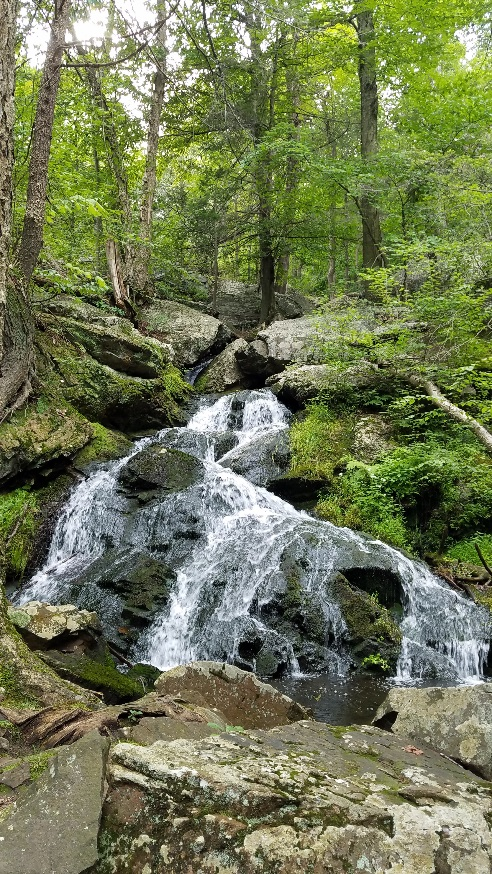
\includegraphics[width=2.25in, height=4in]{images/stream.jpg}
%  \caption{Babbling brook}\label{fig:bablingbrook}
%\end{wrapfigure}

The Town of Cornwall and the Village of Cornwall-on-Hudson have a broad network 
of perennial, intermittent, and ephemeral streams that are admired for their 
beauty. Some are perennial, flowing continuously throughout the seasons, but 
some may dry up during drier periods. These include the Moodna Creek and its 
tributaries flowing from the towns of Blooming Grove and New Windsor; Woodbury 
Creek and its tributaries flowing from the towns of Woodbury and Highlands; and 
Idlewild Creek and its tributaries flowing entirely from within Cornwall. With 
the exception of a few streams, like Clove Creek and the yet-to-be-named creek 
alongside Pagenstecher Park, all streams flow into the Hudson River via the 
Moodna Marsh. All are beautiful, but some are particularly magnificent like Baby 
Brook in Schunnemunk Mountain, pictured at left.

Our streams are also important to habitat health, water quality and 
availability for drinking water and irrigation, flood management, and 
recreational enjoyment. Streams add immeasurably to our residents’ quality of 
life and to the value of our properties. Development can result in the 
alteration of streams or modification of their flows from installation of 
culverts and dams. Development can also increase surface water runoff from the 
reduction of permeable surfaces. These changes can increase flooding, increase 
the deposition of pollutants in our waterbodies, and interfere with habitats 
(see ~\nameref{subsec:streamandriparianhabitat} and 
~\nameref{subsec:floodzones} sections). With our changing climate, 
precipitation has become more variable and extreme in the Northeast, 
exacerbating the deposition of a wide range of contaminants into streams and 
other local waterbodies from increased stormwater runoff.

We are informed of the quality of our streams through various measurements and 
classifications established by the federal government through the Clean Water 
Act and New York State through the Environmental Conservation Law. These 
quality assessments are explained through the following two maps: 
(~\nameref{map:streamclassifications}) and Stream Biomonitoring and 
Priority Waterbodies (~\nameref{map:biomonitoringandprioritywaterbodies})

\subsection*{Stream Classification Map}
Freshwater streams and waterbodies are classified by the DEC based on existing 
or best usage from classes AA or A for drinking water (in green on this map) to 
D, which is not suitable for drinking, swimming, nor for supporting fisheries. 
Streams with a classification of A, B, or C may also have a standard of T (may 
support trout) or TS (may support trout spawning). The description of NYSDEC’s 
streams classifications appears below.
\begin{itemize}
    \item AA or A: Used as a source of drinking water (green)
    \item B: Best usage for swimming and other contact recreation, but not for
        drinking (yellow)
    \item C: Waters supporting fisheries and non-contact activities (orange)
    \item D: Lowest classification (not on map)
\end{itemize}
''Waterbodies that are designated as C(T) or higher (e.g., C (TS), B, A, or AA) 
are collectively referred to as protected streams, and are subject to 
additional regulations and require a State permit for disturbance of the bed or 
banks``~\citep{haeckel2014}. As Cornwall has no streams in the D 
classification, all streams are protected. Other systems of stream 
classification are based on a range of physical conditions, habitat values, and 
human uses.

In the Town and Village, well-shaded cool to cold-water streams with clean 
gravel bottoms are able to support native fish such as brook trout. These 
trout-friendly areas are listed below.
\begin{itemize}
    \item Map sections B4/B5, C4/C5: Mineral Spring Brook is currently listed 
as a Class C stream capable of supporting trout spawning (TS).
    \item Map section B4: Woodbury Creek is currently listed as a Class C (TS) 
stream.
    \item Map sections C2/C3: Moodna Creek is currently listed as a Class B (T) 
stream capable of supporting a trout population.
    \item Map sections C2/C3/C4, D2/D3/D4: Idlewild Creek and its tributaries, 
including Black Rock Forest’s Black Rock Brook are classified as Class C (TS) 
and Class B (TS) streams capable of supporting trout spawning.
\end{itemize}

\includepdf[pages=-,fitpaper]{cornwall_maps/StreamClassifications.pdf}\label{map:streamclassifications}

\subsection*{Stream Biomonitoring and Priority 
Waterbodies}\label{subsec:streambiomonitoring}
Surface water has an ecosystem supporting a wide variety of plant and animal 
life. Since this ecosystem is directly affected by the quality and quantity of 
the water in its environment, or stressors on this environment, water quality 
can be determined through biological monitoring or biomonitoring of the variety 
and number of organisms which inhabit waterbodies. These organisms, such as 
fish, invertebrates and plant life, are catalogued by number and type. The 
results determine if the organisms were collected from clean or polluted water 
and are an indicator of the health and safety of a waterbody. Ongoing 
biomonitoring will reveal changes in water quality over time. When surface 
water and wetlands are polluted, or when groundwater is not adequately 
replenished, it ultimately affects our aquifers; biomonitoring can reveal and 
provide the beginning point for addressing such public health issues. In the 
Lower Hudson Basin, agriculture, urban/storm runoff, municipal discharge, and 
hydrologic modification were found to be the primary sources of impact on our 
streams and waterbodies as of 2008 (NYSDEC 2008).

Every major watershed in New York State is studied on a 5-year schedule as part 
of the \gls{ribs} Program. Water quality standards can be upheld through the 
\gls{spdes} permit program, which issues discharge permits and enforces 
compliance in setting DEC Water Quality Classifications.

This map provides information on the Town's and Village's waterbodies via two 
assessment sources: (1) a biomonitoring water quality assessment conducted by 
Orange County Water Authority (2004-2012) applying the Biological Assessment 
Profile score (BAP) and (2) NYSDEC waterbody assessment completed as of 2008.  
NYSDEC and OCWA categorize the biological assessment of water quality in four 
impact categories based on the BAP score. Parameters for developing a BAP score 
include, among others, species richness and diversity, nutrient types and 
levels, and dissolved oxygen levels. BAP assessments reflect an analysis at a 
specific point in time at a specific location. (Additional information on the 
metrics that form the BAP scores is found in NYSDEC's Fact Sheet on Assessment 
of Water Quality Impact on Streams and Rivers.) 

BAP scores appear below. The quality of the streams in Town and Village ranges 
from Moderately Impacted to Non-impacted. There are no Severely Impacted 
streams, although there are several streams that have not been assessed. They 
are generally in protected areas and are Class A streams.
\begin{itemize}
    \item Non-impacted 10-7.5 – Very good water quality. Virtually unaffected 
    by human disturbance or receiving discharges that minimally affect 
    biota.
    \item Slightly Impacted 7.5 – 5 – Good water quality. The 
    macroinvertebrate community is slightly, but not significantly altered from 
    the pristine state.
    \item Moderately Impacted 5-2.5 – Poor water quality. Fish may propagate, 
    but probably will not survive.
    \item Severely Impacted 2.5-0 – Very poor water quality. Only the 
    strongest, most dominant species will survive.
\end{itemize}

The Moodna Creek and its tributaries are mostly Not Impacted (green lines), 
though some in the southwestern part of town have Slight (Minor) Impacts (pink 
lines). Woodbury Creek is also Slightly Impacted.

\includepdf[pages=-,fitpaper]{cornwall_maps/BiomonitoringandPriorityWaterBodies}\label{map:biomonitoringandprioritywaterbodies}


%***************Geology & Soils******************
\chapter{Geology and Soils}\label{sec:geology}
\section{Bedrock Geology}\label{subsec:bedrock}
\subsection*{Why you need this map}
A region's landscape is greatly influenced by its geology and the processes 
which modify it. The Hudson Valley’s diverse geology contributes to our local 
ecosystems and enables many human activities and industries as well. Gypsum and 
limestone deposits along the Hudson River support cement factories, shale and 
sand and gravel mines dot the valley’s landscape, the "black dirt" region’s 
fertile soils support agriculture, and mountain ridges and other geologic 
features are popular destinations for outdoor recreation. Bedrock and surficial 
geology strongly influence soil properties as well as groundwater and surface 
water chemistry, which in turn influence the type of ecological communities that 
can thrive ~\citep{haeckel2014}. More detailed information of the different types 
of soils found in Cornwall is available in the General Soil Classes chapter of 
this \gls{nri}.

Bedrock is solid rock that typically lies beneath soil and other broken or 
unconsolidated material (regolith). Bedrock is made up of igneous, sedimentary, 
or metamorphic rock, and it often serves as the parent material for regolith 
and soil. A bedrock deposit that occurs at Earth’s surface is called an 
outcrop. The processes of weathering and erosion affect bedrock. Outcrops 
exposed to wind and water are often decomposed, or weathered, over time into 
regolith or smaller particles.1 Knowledge of regional bedrock characteristics is 
important to planning, as it plays an important part in determining the 
viability of well water access and productivity, and large scale slope and grade 
stabilization. More detailed information about Cornwall's wells and aquifers can 
be found in the ~\nameref{subsec:groundwater} section of this NRI.

\begin{figure}
  \begin{centering}
    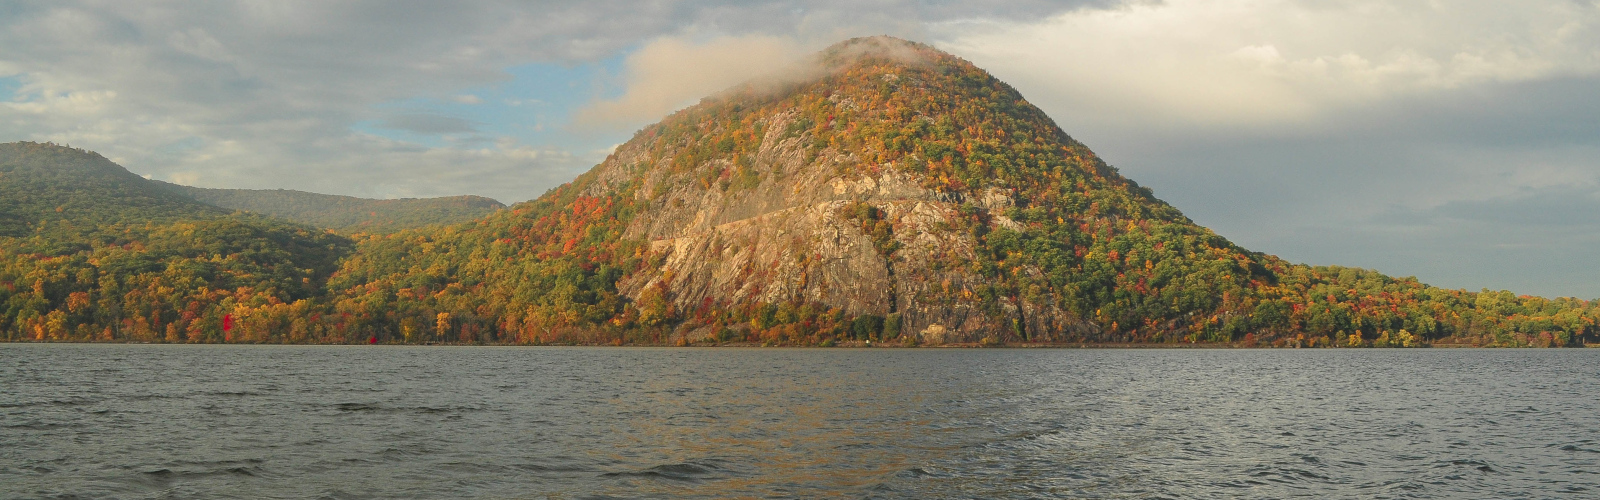
\includegraphics[width=\textwidth]{images/stormking.jpg}
    \vspace{-10pt}
    \caption{Storm King Mountain}\label{fig:stormking}
  \end{centering}
\end{figure}

Surficial geology is the study of landforms and the geologic materials lying on 
top of the bedrock. These materials can be sand and gravel, clay and silts, and 
glacial tills. Mapping these glacial deposits and other aspects of surficial 
geology provides important information to aid land use decisions, such as 
building roads and other structures; safeguarding drinking water; preparing for 
natural disasters; protecting wildlife and their habitats; and mitigating the 
effects of geologic hazards. Such information benefits residents and industry 
alike.

\includepdf[pages=-,fitpaper]{cornwall_maps/BedrockGeology.pdf}\label{map:bedrockgeology}

\subsection*{Bedrock and Surficial Geology of the Town of Cornwall and the 
Village of Cornwall-on-Hudson}
Cornwall has its share of stunning magnificent granite outcroppings in Storm 
King State Park that have captured the imagination of settlers, rusticators, 
and tourists for generations. This map identifies the four main types of 
bedrock to be found in the Town of Cornwall and Village.
\vspace{4mm}
%0.4\textwidth
\begin{wrapfigure}{r}{0pt}
    \centering
        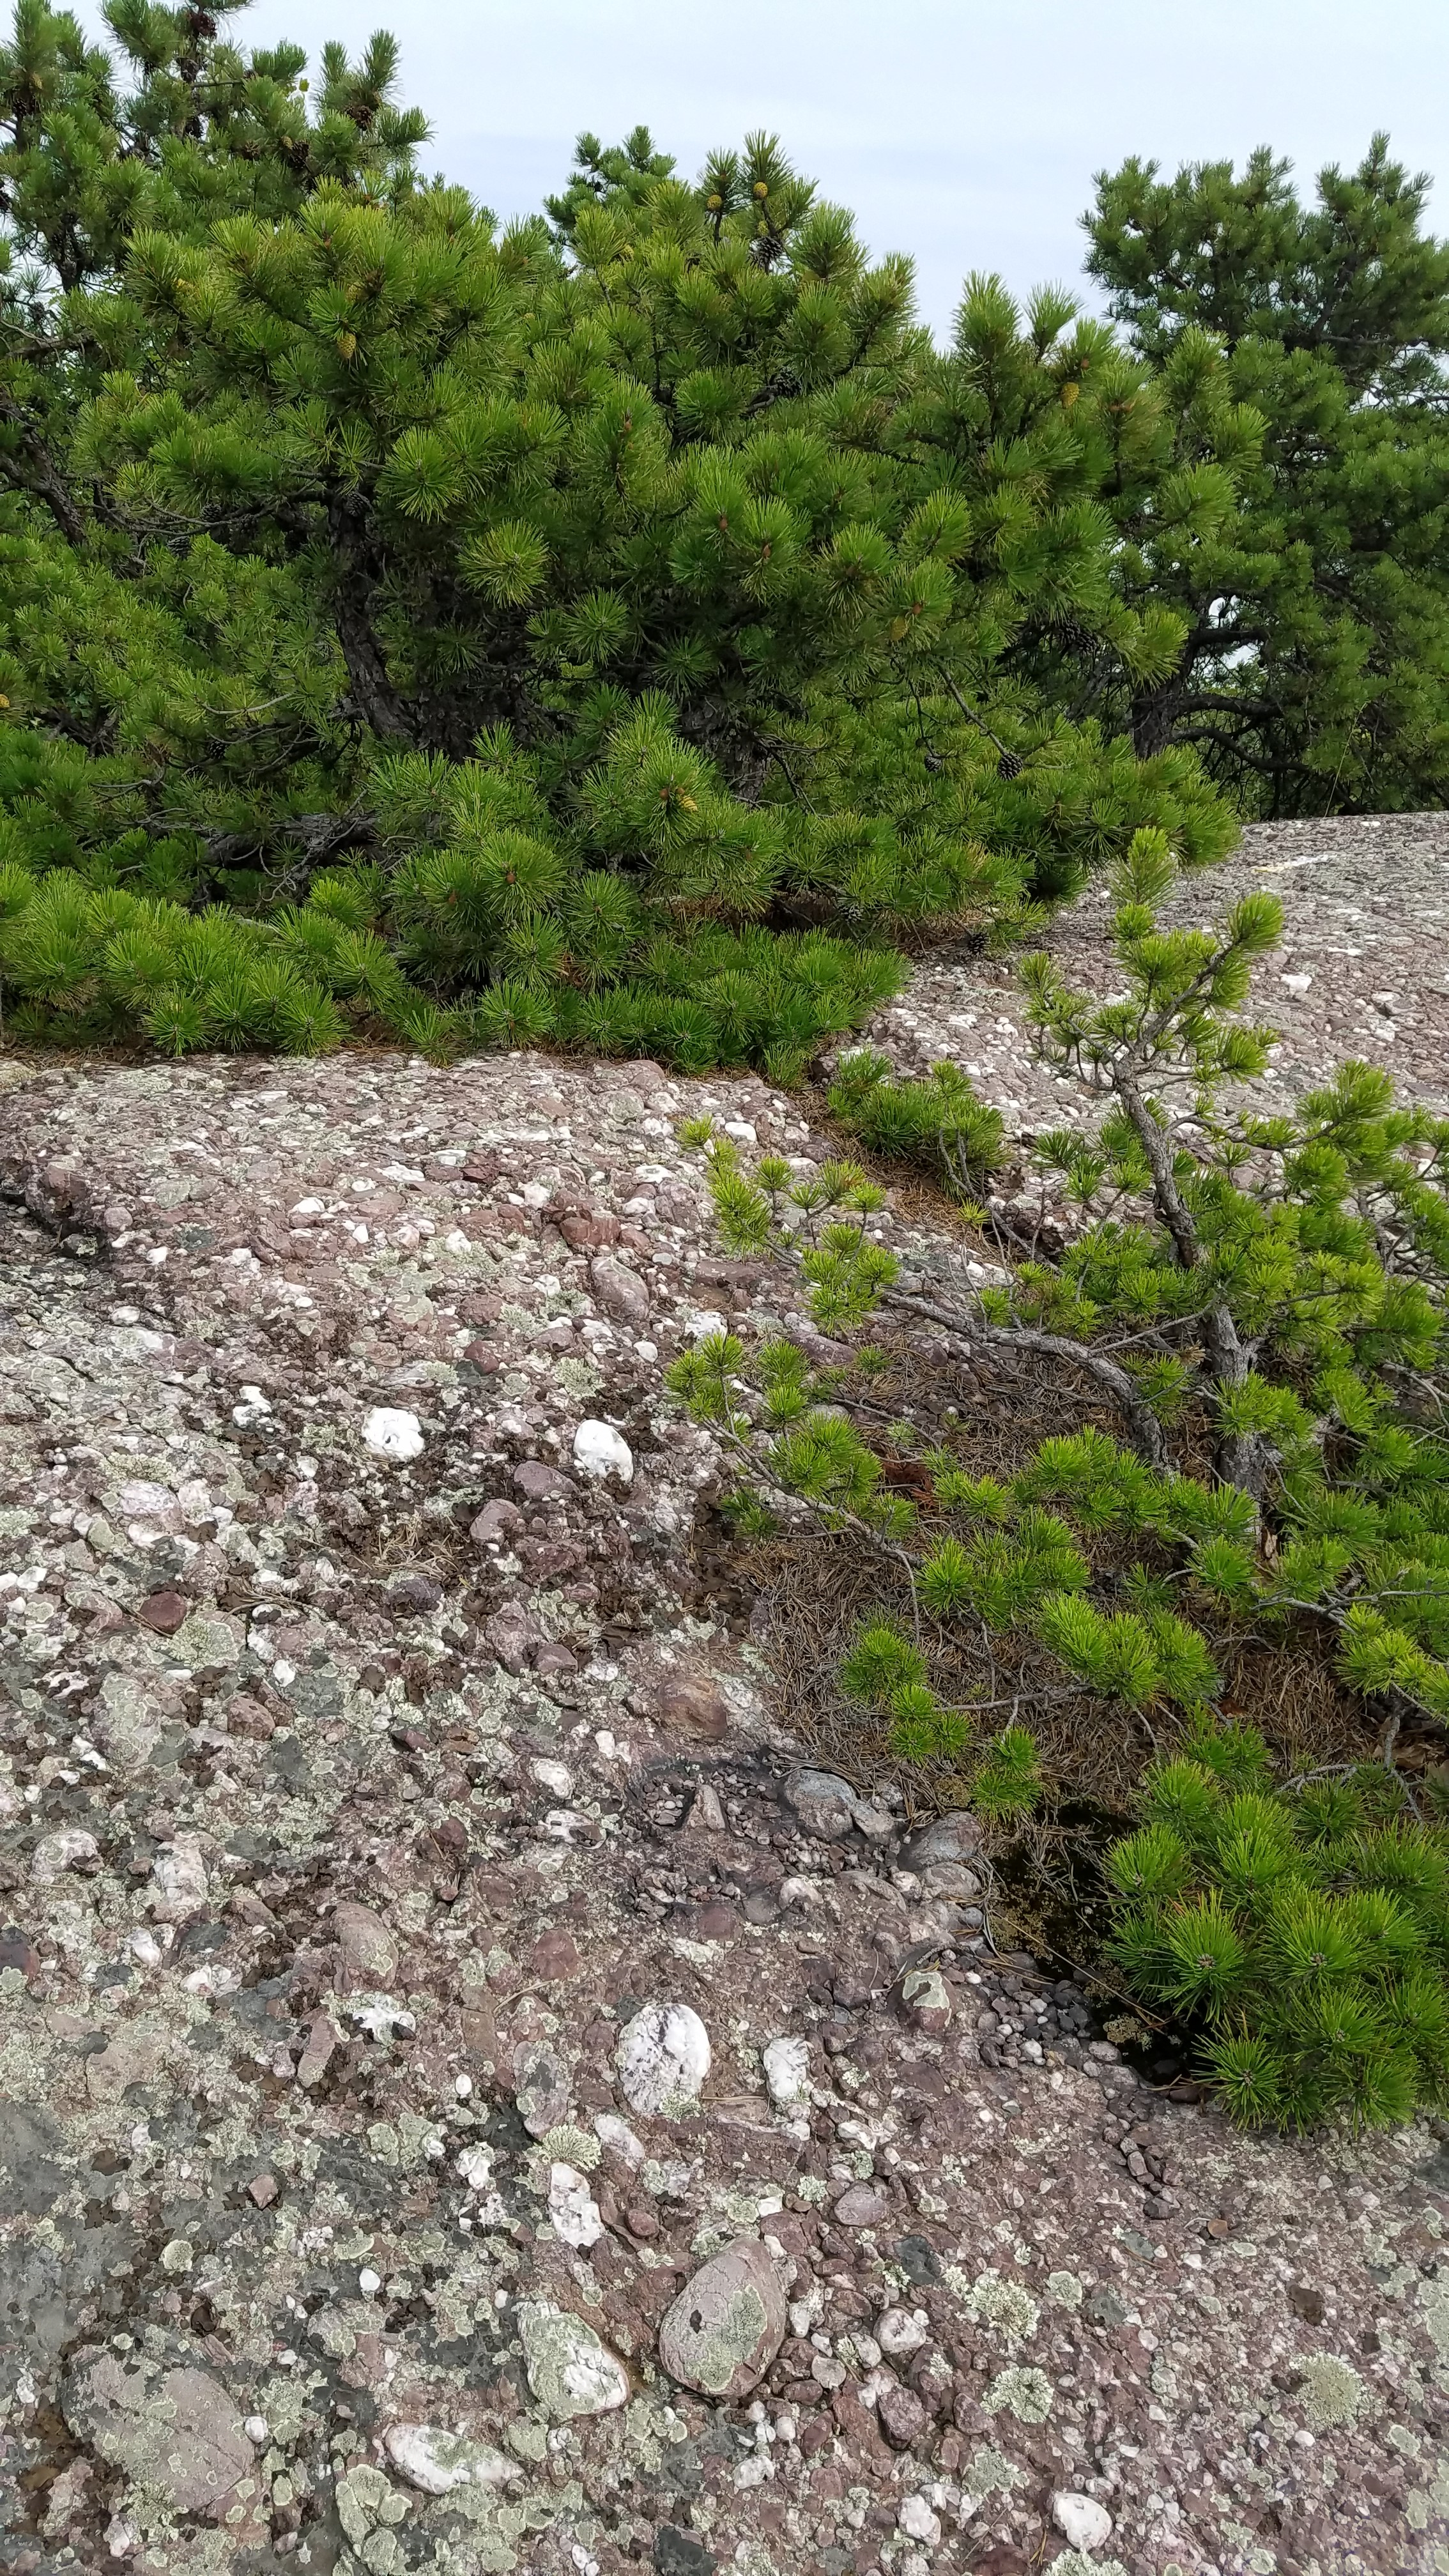
\includegraphics[width=0.4\textwidth]{images/Pudingstone.jpg}
        \caption{Schunnemunk Conglomerate (puddingstone)}\label{Schunnemunk Conglomerate}
\end{wrapfigure}
\begin{itemize}
    \item The southeast portion of Cornwall, which resides in the Hudson 
Highlands, is composed of undifferentiated gneiss, granite and granitic gneiss. 
Storm King Mountain is primarily composed of granite (granitic gneiss) and a 
small band of mafic gneiss.
    \item In the town's southwest, granite gives way to the Middle Devonian 
layered sandstone and shale of the Schunnemunk ridge.
  \item Much of the Town and Village’s more developed areas and commercial corridors 
    are underplayed by graywacke and shale bedrock within the Mount Merino and 
    Austin Glen formations (true?). The western part of the town north of 
    Schunnemunk Ridge is also mostly greywacke, shale, and siltstone.
    \item Significant portions of land on either side of the Moodna Creek are 
    underlayed by Quaternary alluvium and glacial drift
\end{itemize}
The surface of the bedrock varies in depth from surface exposure to greater 
than 100 feet deep. A report by the \gls{ocwa} found that 
wells drilled into bedrock units within the Town are not highly productive. 
Most residential wells within the Town are low yield bedrock wells. No high 
yield bedrock wells were identified during this study.

\paragraph{The Village of Cornwall on Hudson} has two main geologic features bisecting the 
Village: granitic gneiss and graywacke and shale. There is a small band of 
mafic gneiss in the southwest corner of the Village.

\section{Steep Slopes}\label{subsec:steepsloes}
\subsection*{Why you need this map}
The topic of steep slopes is an important consideration for municipalities when 
planning development of any kind. Steep slopes will also determine the physical 
limitations of development within a given municipality. The major concerns 
around slopes are erosion and flooding, which both impact the integrity of the 
natural and built environments around them. Trees and other vegetation hold the 
soils in place and can mitigate the effects of rain and wind on steeply sloped 
terrain. Allowing development or otherwise disturbing these areas makes soil 
unstable and more prone to erosion, and can have unintended adverse impacts on 
structures, roads, and natural and man-made drainage systems. In addition to 
posing a hazard to nearby structures and transportation corridors, the erosion 
of steep slopes can also greatly impact water quality, as loosened soil is 
washed into streams increasing water turbidity and sediment deposition. Any 
pollutants present in slope soil will also be spread into drainage systems in 
this fashion. This has the potential to negatively impact surface drinking 
water sources.

Steep slopes are valuable resources and are notable for their scenic and 
environmental qualities, which can bring special character to a community. 
Ravines and steep hillsides often provide scenic vistas, hiking opportunities, 
and natural beauty that can boost eco-tourism and property values. In many 
cases there is limited accessibility to steeply sloped terrain, and these areas 
provide vital undisturbed habitat for many plant and animal species. Steep 
slopes and cliffs can also form microclimates which can support unique and rare 
specimens of plants and animals. 

\begin{wrapfigure}{l}{0.6\textwidth}
    \hspace{-2mm}
        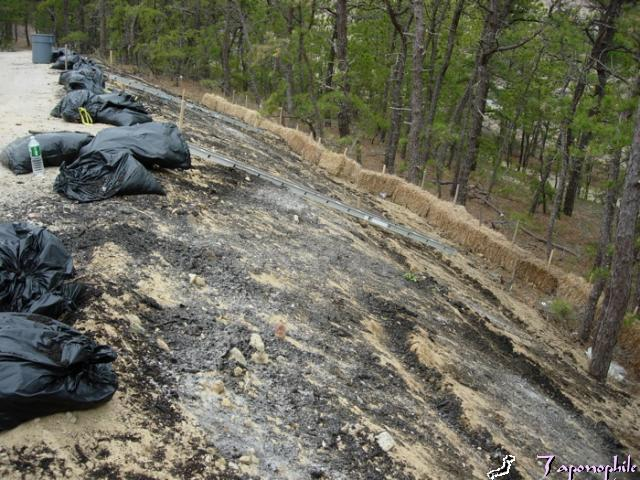
\includegraphics[width=0.5\textwidth]{images/compost222.jpg}
  %\caption{Watershed}
    \hspace{-2mm}
\end{wrapfigure}
The steepness of a slope is usually expressed as a percentage (rise over run). 
In general, the stability of slopes is determined by their grade and length, 
but also by their soil geology, amount of vegetative cover and the particular 
climate they are exposed to. Defining what constitutes “steep” for the purposes 
of slope regulation is at the discretion of each municipality, provided that the 
definition is reasonable. The USDA Natural Resources Conservation Service and 
numerous New York State municipalities more or less adhere to the following 
characterizations of steep slopes:

\begin{table}
\begin{center}
\begin{tabular}{ | p{0.2\textwidth} p{0.8\textwidth}| } 
\hline
Minor slopes < 8\% &
    \begin{itemize}
    \item Minor slopes are best suited for development and less costly to 
    develop; ponding, runoff, and erosion may be a problem on nearly level 
    slopes from 0-2 percent, unless the soils are well drained
    \item Erosion can occur on slopes as slight as 2-3 percent, depending on
    soils.
    \end{itemize}
    \\
\hline
Moderate Slopes 8-15\% &
    \begin{itemize}
        \item Present moderate septic problems because of possible seepage.
        \item Erosion potential exacerbated by the increase in grade
    \end{itemize}
    \\
\hline
Steep Slopes > 15\% (Very Steep Slopes >25\%) &
    \begin{itemize}
    \item Slopes of 15\% and above are generally considered to be more 
    vulnerable to soil erosion, sedimentation, and other problems than more 
    gently sloping areas, with vulnerability increasing with steepness
    \item Slopes greater than 15 percent have soils that tend to be thin and 
    less fertile
    \item Many municipalities have significant land use restrictions for slopes 
    of over 15\%
    \item Construction on such areas can increase the sediment load of streams 
    100 fold
    \item Slopes of  >25\% should be left in a natural condition, carefully 
    maintained in grass or tree cover, or used as pastureland
    \end{itemize}
    \\
\hline
\end{tabular}
\end{center}
\caption{Adapted from \href{http://www.chathamtownship-nj.gov/images/CTEC/NRI1999/slopesadd090704.pdf}{Chatham Township Environmental Commission, 2014}\label{tab:steepslopes}}
\end{table}
\subsection*{Steep Slopes Map}\label{subsec:steepslopes}
The slope designations on this map are broken down into three grades. Green 
indicates slopes of 8-15\%, yellow indicates slopes of 15.1-25\%, and red 
indicates slopes of greater than 25.1\%. The white areas are areas that are 
below 8\% of slope. A considerable amount of the land within Cornwall's borders 
is classified as steeply or very steeply sloped. The most significant areas of 
very steep slopes are encompassed within the borders of Schunnemunk Mountain 
State Park, Storm King State Park, and the Black Rock Forest Consortium. 
Outside the borders of these protected areas, however, there are numerous areas 
of steep slopes within both the town and village borders. Paired with the USDA 
NRC slope concerns mentioned above, municipal planning officials should 
primarily concern themselves with the yellow and red areas on this map when 
making decisions about land development or tree and vegetation removal.

Significant portions of the Village of Cornwall-on-Hudson are also 
characterized by steeply or very steeply sloped terrain. Residential areas 
along Mountain, Maple, and Deer Hill Roads as well as the Boulevard are 
potentially impacted by the slope considerations discussed in the chart above. 
The bluffs overlooking the Hudson River to the East account for the remainder of 
the steeply sloped land in the Village and erosion is currently a problem in 
certain areas where road and residential development exists. Other steeply 
slopes areas in the Town of Cornwall are mainly to be found bordering the Moodna 
Creek and along the residential corridor of Angola, Mine Hill, and Mineral 
Springs Roads. There are locations along the Moodna Creek where significant 
erosion due to the slope of the land and proximity to the creek has occurred. 
These areas will continue to pose a challenge to future town governments, 
departments, and planning boards.

It should be noted that the town of Cornwall zoning code currently considers 
slopes of >25\% to be inappropriate for development. However, given the 
challenges of increased erosion from heavier rain events due to climate change, 
the town should consider revisiting this criterion. Many municipalities have a 
steep slope zoning overlay as part of their general zoning code. Cornwall's 
existing Ridge Preservation zoning overlay focuses only on the largely 
undeveloped, mountainous terrain within the town’s borders. Given that 
significant parts of the town and village outside of that overlay are steeply 
sloped, Cornwall should consider developing a steep slope overlay to ensure 
careful consideration and management of development in these areas. For more 
information regarding recommendations for zoning, see the ~\nameref{subsec:zoning}
in this NRI.

\includepdf[pages=-,fitpaper]{cornwall_maps/SteepSlopes.pdf}\label{map:steepslopes}

\section{Soils}\label{subsec:soils}
\subsection*{Why you need these maps}
Familiarity with the characteristics and different classes of soil is an 
essential starting point to understanding the natural processes that influence 
our environment, and soil information both drives and reflects the uses imposed 
on it by human activities. Whether a soil is acidic or alkaline, loamy, sandy, 
clayey, deep or shallow defines its natural functions. It is important to 
consider these characteristics when a municipality is considering development 
and conservation plans. Soils function to regulate and filter water flow, 
decompose vegetative matter and other wastes, provide nutrients for agriculture, 
and support infrastructure. Soil data can play an important role in agriculture 
and forestry, as it tells us what plants can grow in a certain area and what 
level of irrigation and fertilization they may need. \textbf{Specific soil 
properties are critical factors to consider in land use planning: whether it is 
appropriate or feasible to build, whether septic systems or other types of 
wastewater treatment can or must be utilized, or how much surface area should be 
left in a permeable state}. They can also dictate whether certain building or 
foundation materials would be subject to corrosion by the pH character of the 
surrounding soil. 

\begin{wrapfigure}{l}{0.7\textwidth}
    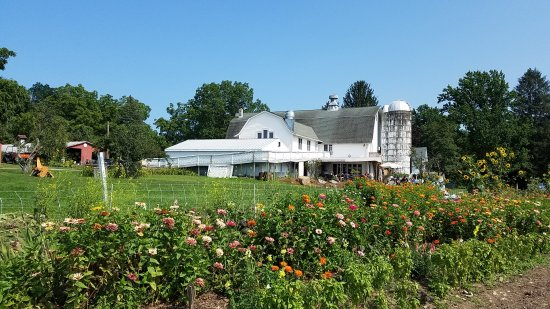
\includegraphics[width=0.6\textwidth]{images/asdasd.jpg}
  \caption{Watershed}
\end{wrapfigure}
Once polluted or depleted, soils can require long periods of 
replenishment/remediation or, worse, need to be abandoned. Recent studies have 
shown that soils, particularly adjacent to roadways, are vulnerable to salt and 
other chemical and heavy metal runoff. Depending on drainage characteristics, 
nearby streams and other bodies of water can also be impacted to the detriment 
of their dependent organisms. Stormwater drainage infrastructure can slow the 
degradation of soils adjacent to roadways as well. Run off from cold weather 
treatments for road surfaces is increasingly being recognized as a threat to 
soil quality adjacent to roads and can impact water quality of nearby streams 
and lakes. It is appropriate for municipalities to consider alternative 
treatments for road surfaces. 

In cases where soil quality creates areas of prime agricultural value or 
supports habitat for rare or endangered species, it may be determined that these 
areas are valuable enough that they should not be subject to commercial or 
residential development.

\includepdf[pages=-,fitpaper]{cornwall_maps/GeneralSoilClasses.pdf}\label{map:generalsoilclasses}

\subsection*{General Soil Classes Map}\label{subsec:generalsoil}
The General Soil Classes map focuses on the relative agricultural utility of 
the soils in our area. These classifications are determined by criteria set by 
the U.S. Department of Agriculture. There are a number of small patches of 
Areas of Prime Farmland (Pink) and Prime Farmland If Drained (Purple) within 
the borders of Cornwall, often contiguous to each other. These soils possess 
the most ideal combination of physical and chemical characteristics for 
producing agricultural products and growing feed for livestock. Looking at the 
~\nameref{map:calcaerousandglacialoutwashsoils}, we see that there is often a 
correlation between prime farmland and the presence of glacial outwash which 
consists of fertile soil material, as well as sand and gravel which aid in 
drainage.

Soils of Statewide Importance (Green) do not meet the criteria for Prime 
Farmland (or Prime Farmland if Drained), but still possess significant mineral 
loads that can support agriculture under the right conditions. Looking at the 
~\nameref{map:calcaerousandglacialoutwashsoils}, we see a correlation between these 
soils of statewide significance and the presence of calcareous and somewhat 
calcareous soils.

There are two very small deposits of black dirt/organic soil (Grey) in Cornwall, 
located in sector B2 on the ~\nameref{map:generalsoilclasses}. These soils are highly 
fertile and contain high levels of organic matter and chemical nutrients. The 
dominant soil class shown on the ~\nameref{map:generalsoilclasses} map, however, is 
Non-Agricultural (Yellow). These areas are predominantly located in and around 
the mountainous and rocky areas of Storm King and Schunnemunk Mountain state 
parks and ridgelines of Black Rock Forest where the soil coverage is 
comparatively shallow. It should be noted that much of the areas identified as 
Prime Farmland, Prime Farmland if Drained, and Soils of Statewide Importance are 
generally the location of residential and light commercial development within 
the Town. The Town should consider identifying any undeveloped prime farmland 
that may remain and prioritizing it for preservation or agricultural use. See 
the ~\nameref{map:landcover} chapters in this NRI for more detail.

\includepdf[pages=-,fitpaper]{cornwall_maps/CalcareousandGlacialOutwashSoils.pdf}
\label{map:calcaerousandglacialoutwashsoils}
\subsection*{Calcareous and Glacial Outwash Soils Map}\label{subsec:calcareous}
The soil types in the Cornwall/Cornwall-on-Hudson region are dominated by silt, 
rock outcrops, gravel, and gravelly silt. These soils result from glacial till 
deposits and together form a drainage sequence from the excessively drained, 
mountainous soils, to the poorly drained silts. The ~\nameref{map:calcaerousandglacialoutwashsoils}
map shows that, in Cornwall, the Calcareous (magenta) and Somewhat 
Calcareous (Yellow) soils, with their potential to provide habitats for rare 
species, are located throughout the lowland areas of the Town and Village. These 
areas are also characterized as “Soils of Statewide Importance” which means they 
also have agricultural value even though they do not meet the criteria for prime 
farmland and prime farmland if drained.

In geological terms, calcareous soils are those which contain a high proportion 
of calcium carbonate in the form of calcite or aragonite (limestone). 
Calcareous, or alkaline, soils serve as a habitat for a broad diversity of 
organisms and are often associated with uncommon habitats and rare species. 
Given their relatively high pH (7.5 to 8.4) they are not ideal for most 
agricultural uses. Somewhat Calcareous soils can have a pH as low as 6.5, and 
can function as agricultural land with the introduction of manure and other 
nitrogen-rich soil additives.


\part{Cornwall's Future?}
%***************Climate Change******************
\chapter{Climate Conditions and Projections}\label{sec:climate}
Our climate is changing and the associated impacts are being felt from the 
global level down to our local community. Increasing temperatures, rising sea 
level, and changing precipitation patterns are leading to cascading and 
interconnected impacts on our health, our environment, and our economic 
vitality. We are experiencing these climate hazards as flooding, heat waves, 
and drought. Understanding how these changes are affecting our community will 
help us address their impacts by increasing our resilience through smarter 
decision-making, land-use planning, and adaptation. Natural resources are an 
important asset in planning for resilience, managing climate risks, and 
recovering from extreme weather events ~\citep{haeckel2014}. A brief overview of 
the effects of our changing climate follows; additional background information 
is found in the appendix section.
\par
We are seeing \textbf{temperature} increases that are making our summers hotter 
and our winters warmer and shorter; annual average temperatures have increased 
\textcolor{red}{2}$\si{\degree}$F and winter temperatures have increased 
\textcolor{red}{5}$\si{\degree}$F in New York since 1970. Temperature fluctuations 
are impacting the growing season of our food crops and the beauty of our 
autumnal leaf season. These changes, in turn, are impacting our produce and 
tourism economies.
\par
The incidence of extreme temperatures is also increasing. ``By mid-century, 
the Hudson Valley could annually experience 3-12 days above 
\textcolor{red}{95}$\si{\degree}$F, and four to seven heat waves that last 1-2 days 
longer than average'' ~\citep{Zemaitis2018}. ``Climate Impacts on Human Health'' 
notes that these increases will put in danger the lives of our vulnerable 
residents—our children and elders—from extreme heat and poor air quality. The 
\textit{National Climate Assessment} further notes that increasing temperatures 
are projected to result in decreased air quality from increase ground-level 
ozone and/or particulate matter air pollution. ``Ground-level ozone (a key 
component of smog) is associated with many health problems, such as diminished 
lung function, increased hospital admissions and emergency room visits for 
asthma, and increases in premature deaths'' ~\citep{melillo2014}. 
Ground-level ozone and particulate air matter will be of special concern in 
Orange County because cars are the greatest source of air pollution, given the 
high single-occupancy vehicle rate and commuting distances in Orange County; 
traffic on Stewart Airport, I-84 and I-87, and nearby power plants will also 
play a role. (Orange County is fortunate to have seen a general improvement in 
air quality since 1999 across many ~\gls{naaqs} metrics, resulting in a decreased 
number of unhealthy days for people suffering from asthma, lung disease, and 
heart disease as well as for older adults, children, people engaged in outdoor 
activities, and the general population ~\citep{aircompare, ocnysenvironmental}. 
\par
Our precipitation patterns are also changing. The Northeast and New York have 
seen a 71\% increase in heavy precipitation events between 1958 and 2012, that 
have resulted in more frequent and costly flooding \citep{melillo2014}. 
While the reduction in forested and undeveloped land cover plays a role in 
increased flooding, even these pervious areas cannot absorb the intense rainfall 
from heavy precipitation events, becoming water-logged and reducing the amount 
of water that reaches our aquifers. Our aquifers are also seeing a lower 
recharge rate due to the reduction in snowpack, caused by increased winter 
temperature. Snowpack decline is also negatively impacting our winter 
recreational industries and economy.
\par
Rising sea levels are affecting all waterfront communities, including Hudson 
River estuary communities. ``Since 1900, sea level in the lower Hudson has 
risen one foot'' ~\citep{haeckel2014}, with an additional projected rise of up 
to 75 inch, or over six feet, for the Lower Hudson Valley by the end of this 
century ~\citep{horton2014climate}. Rising sea levels will lead to flooding along 
estuary shorelines and tidal tributary waters, particularly in low lying areas. 
Flooding will be compounded by heavy storm surges, such as those we experienced 
from Hurricanes Irene and Sandy, and intense rainfall leading to additional 
tributary and stormwater flooding.

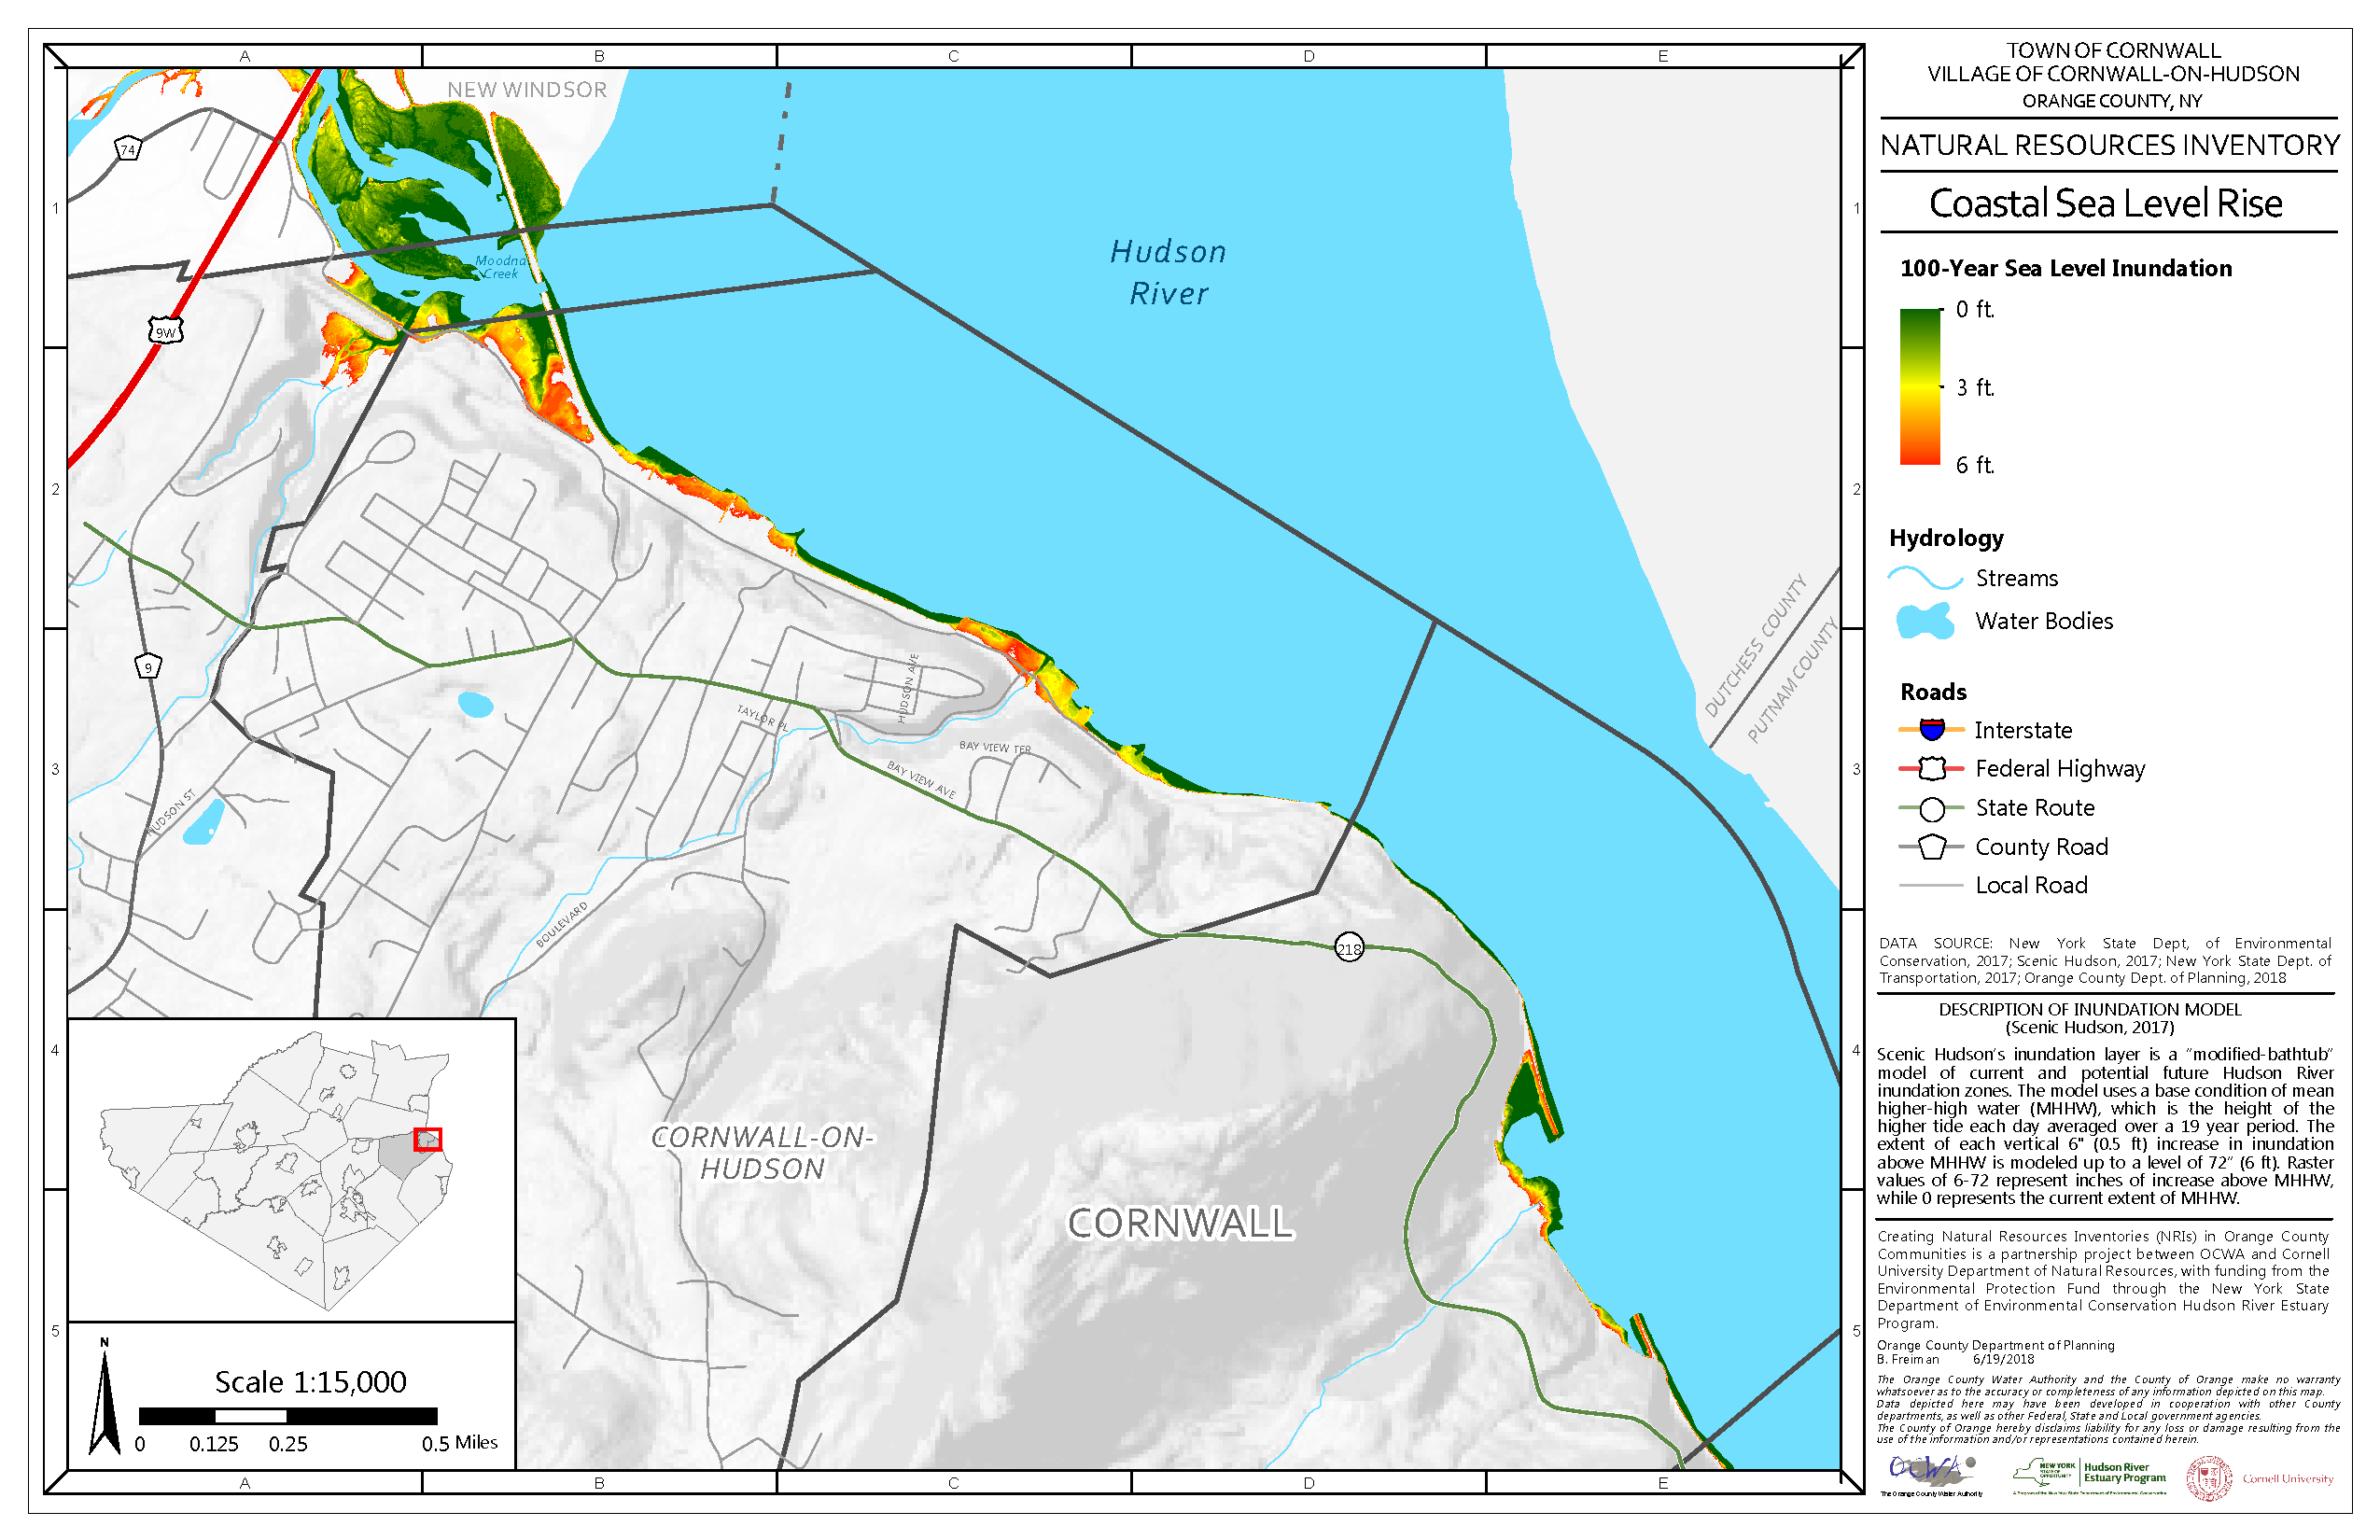
\includepdf[pages=-,fitpaper]{cornwall_maps/CoastalClimateChange.pdf}\label{map:coastalclimatechange}
\subsection*{Coastal Sea Level Rise Map}
The Village of Cornwall-on-Hudson has significant shoreline on the Hudson River 
and is vulnerable to sea level rise. This image shows two important community 
assets: Donahue Memorial Park in the Village and the wastewater treatment plant 
in the Town at the mouth of the Moodna (source: New York Climate Change Science 
Clearinghouse).
\par
The Coastal Sea Level Rise map depicts the areas of future inundation that 
Village and Cornwall residents would experience from a rising Hudson River. In 
a 3-foot sea level rise, 100-year flood scenario (yellow on the map), key 
portions of the wastewater treatment plant are submerged and Shore Road is 
almost inaccessible; we lose roughly half of Donahue Memorial Park to the 
Hudson. In a 6-foot sea level rise scenario (in red), the entire wastewater 
treatment site is in the Hudson and Donahue Memorial Park ceases to exist. Our 
access to the river becomes the train tracks.
\par
In addition to the riverfront inundation modeled in the map, this image shows 
the resulting flooding that would reach inland (orange) as a result of a 6-foot 
sea level rise. 

\subsection*{Becoming a Climate-Resilient 
Cornwall}\label{subsec:climateresilient}
We are already seeing the costly effects of our changing climate and have 
responded to these impacts in different ways. For example, we have protected 
sewage treatment facilities by raising their height, repaired drainage 
destroyed by heavy storms, cleared away left-over storm debris, and cleaned up 
our flooded houses. Understanding the best-case and worst-case scenario 
projections, however, have armed us with the ability to take proactive measures 
to make our community more resilient to the impacts of climate-caused hazards. 
\par
Below is a short list of actions that the New York State Climate Smart 
Communities Program recommends that communities like ours pursue as part of any 
resiliency planning and as a means of responding to the expected federal and 
state mandates for ``strong coastal and floodplain construction standards and 
pre-disaster mitigation planning.''
\begin{enumerate}
    \item Conduct an assessment of municipal and county documents, where 
applicable, to determine the degree to which plans, ordinances, and strategies 
incorporate resiliency planning.
    \item Develop or update a vulnerability assessment to identify ``vulnerable 
    populations, businesses, infrastructure, and natural resources.'' The 
    assessment process assists municipalities with building their knowledge and 
    ability to plan for climate-caused hazards.
    \item Engage the public in identifying the effects of historic storms 
    and make available to the public ``information on the natural and 
    beneficial 
    functions of floodplains, wetlands, and green infrastructure.'' 
    Periodically conduct storm preparedness outreach to residents and 
    businesses.
    \item Develop or update a heat emergency plan. Explore the expansion of 
    cooling centers.
    \item Increase shading in public spaces with trees and other structures.
    \item In the municipal comprehensive plan, reference other plans that 
    address hazard exposure reduction and reduction in property loss, such as a 
    local multi-hazard mitigation plan, floodplain management plan, local 
    waterfront revitalization plan, stormwater management plan, natural 
    resources inventory/plan, etc. Include resilience in the comprehensive 
    plan's mission, vision, or goals.
    \item Incorporate future flooding and preferred adaptation strategies into 
    local planning. Promote best practices and technologies to address flooding.
    \item Right size culverts.
    \item See financial assistance for flood adaptation
    \item Maintain existing natural infrastructure. Use natural vegetated 
    buffers to protect assets from flood risk. Identify and conserve natural 
    areas contributing to stormwater management. 
    \item Encourage building and permitting officials to complete training on 
    retrofitting flood-prone residential buildings.
    \item Implement a program to conserve and reuse water.
    \item Create a source-water protection program.
    \item Establish special area ordinances for habitat preservation. 
    \item Reduce ~\gls{ghg} emissions by supporting and implementing renewable 
    energy and energy efficiency projects.
\end{enumerate}
\nocite{climateexplorer}
\nocite{climatesmart}
\nocite{climateimpactshealth}
\nocite{nysag2014}
\nocite{mhredcstrategic}
\nocite{cscresiliency2014}
\nocite{ocnysenvironmental}
\nocite{degaetano2011}

%*******Proposed Fossil Fuel Infrastructure*****
\chapter{Proposed Fossil Fuel Infrastructure}\label{sec:fossil}
\subsection{Proposed Pilgrim Oil Pipelines}\label{subec:pilgrim}
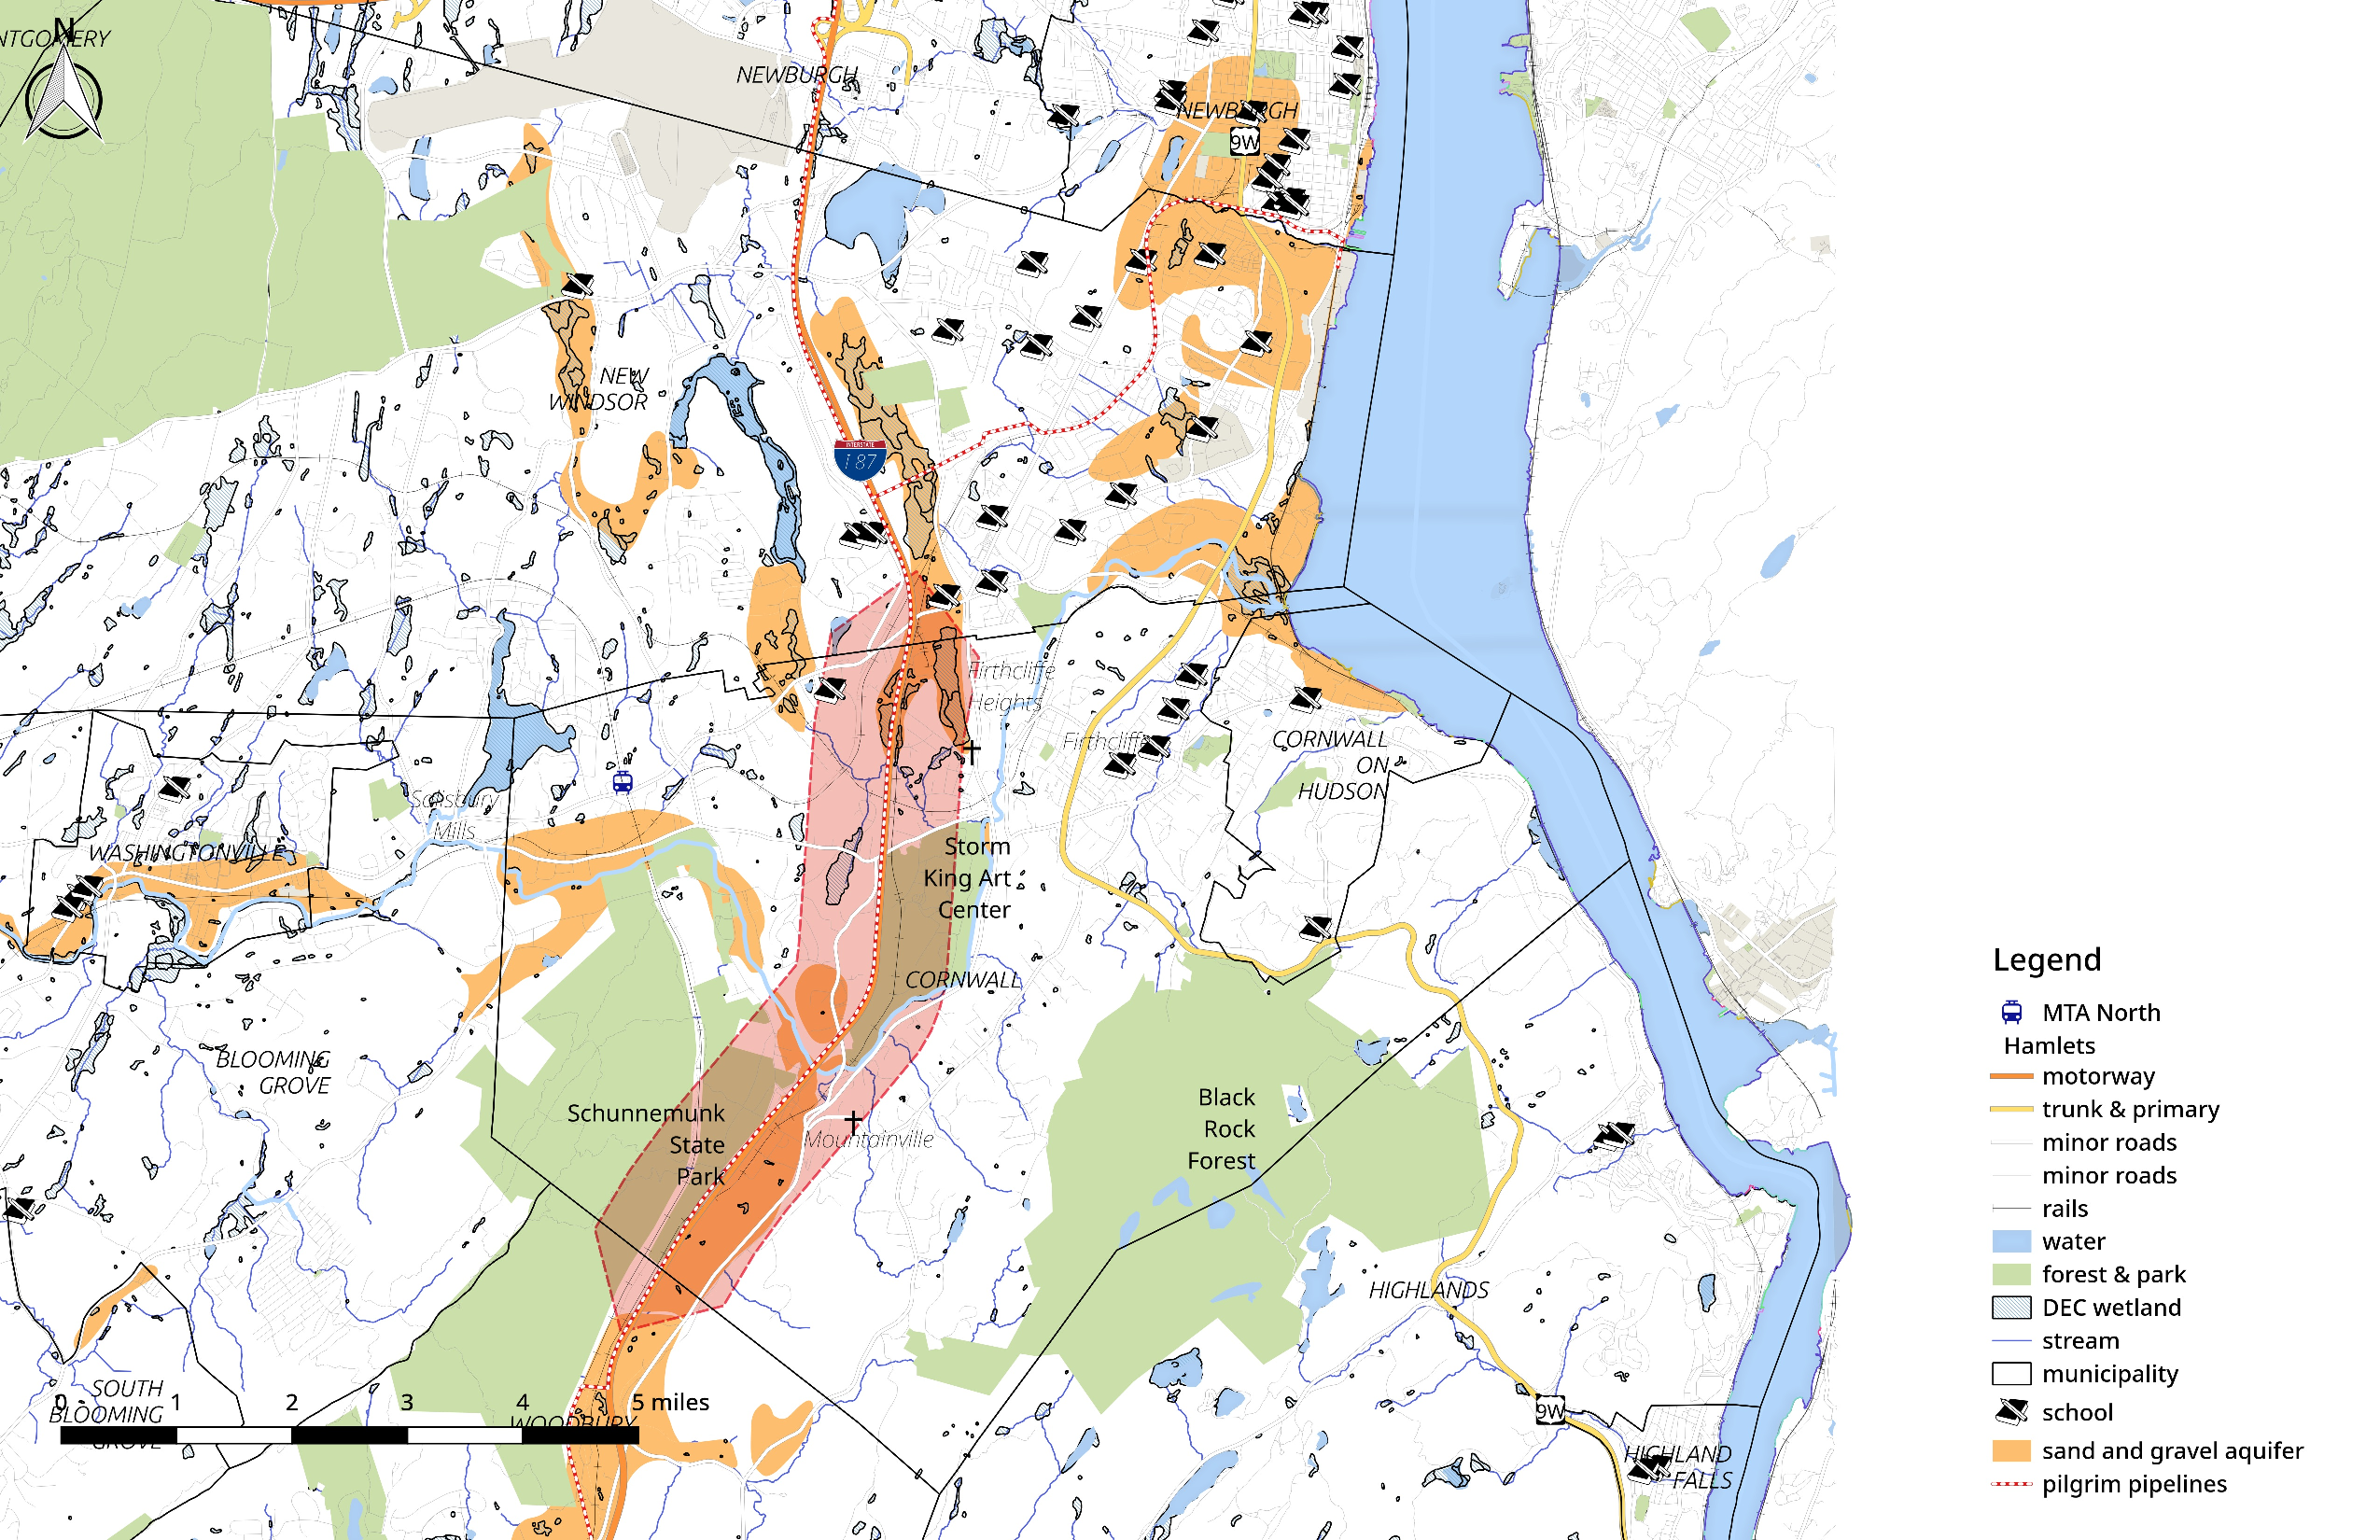
\includepdf[pages=-,fitpaper]{cornwall_maps/proposed_pilgrim_oil_pipelines.pdf}
\label{map:proposedoilpipelines}
This map shows planned fossil fuel infrastructure and its proximity to sand and 
gravel aquifers, public institutions and other important natural areas. The 
proposed Pilgrim Oil Pipelines would carry both refined petroleum products 
(gasoline, diesel, heating oil, and kerosene) and crude oil underground between 
Linden, NJ and Albany, NY along the NYS Thruway. The project’s co-lead 
agencies, \gls{nysta} and \gls{nysdec} determined the project would have 
``potentially significant impact on the environment'' and hence issued a 
``Positive Declaration`` under Article 8 of the Environmental Conservation 
Law. A ''Positive Declaration`` requires a full Environmental Impact Statement 
(EIS) with a public scoping requirement and public comment period. The pipelines 
would be 356 miles long, with 116.4 miles being in New York State, with 5 
laterals, 4 pump stations, 10 meter stations and 35 permanent access roads. 
During construction there would be 50 temporary access roads and 7 major 
construction zones/staging areas. Each pipeline would be 20 inches in diameter 
and have the potential to transport 8.4 million gallons per day (200,000 
barrels/day). The pipelines would cross 257 waterways and would be run very 
close to water supplies of municipalities. There are also 296 (9.2 linear miles)
crossings of wetlands; including 25 crossings of \gls{nysdec}protected 
freshwater wetlands (approximately 19 along mainline pipelines and 6 along 
laterals). If pipelines were constructed more solidly or their leak detection 
systems were better then this might not be an issue. Recent data suggests that 
pipelines are prone to leaking and sometimes days go by before a leak is 
detected and is responded to.

From the south, the pipelines would run adjacent to Schunemunk State Park and 
Storm King Arts Center which are important recreation sites and home to flora 
and fauna. A little less than 5 miles (4.6) of the pipeline would bisect the 
Town’s boundary. Much of the pipelines in Cornwall would be located on top of 
sand and gravel aquifers. The pipeline also traverses across 4 waterways in 
Cornwall and 5 points that are designated as high yielding well sites would be 
within one mile of the proposed pipelines. Two churches and the Cornwall High 
School are within a 0.5 mile risk zone as can be seen on the map. The half mile 
risk zone was added to the map to give viewers an idea off how close they would 
be to the dangers of a leak or an explosion.

In the Town of New Windsor, the lateral would run adjacent to the Quassaick 
Creek which is an important habitat for eel species. Much of the pipelines’ path 
would be built on top of a sand and gravel aquifer which is described as 
“Stratified clay and silt with no or thin layers of sand and gravel at land 
surface and below the water table”. A spill on top of a sand and gravel aquifer 
would risk serious contamination of the groundwater.

\subsection{Proposed Anchorage Sites on the Hudson 
River}\label{subsec:anchorages}
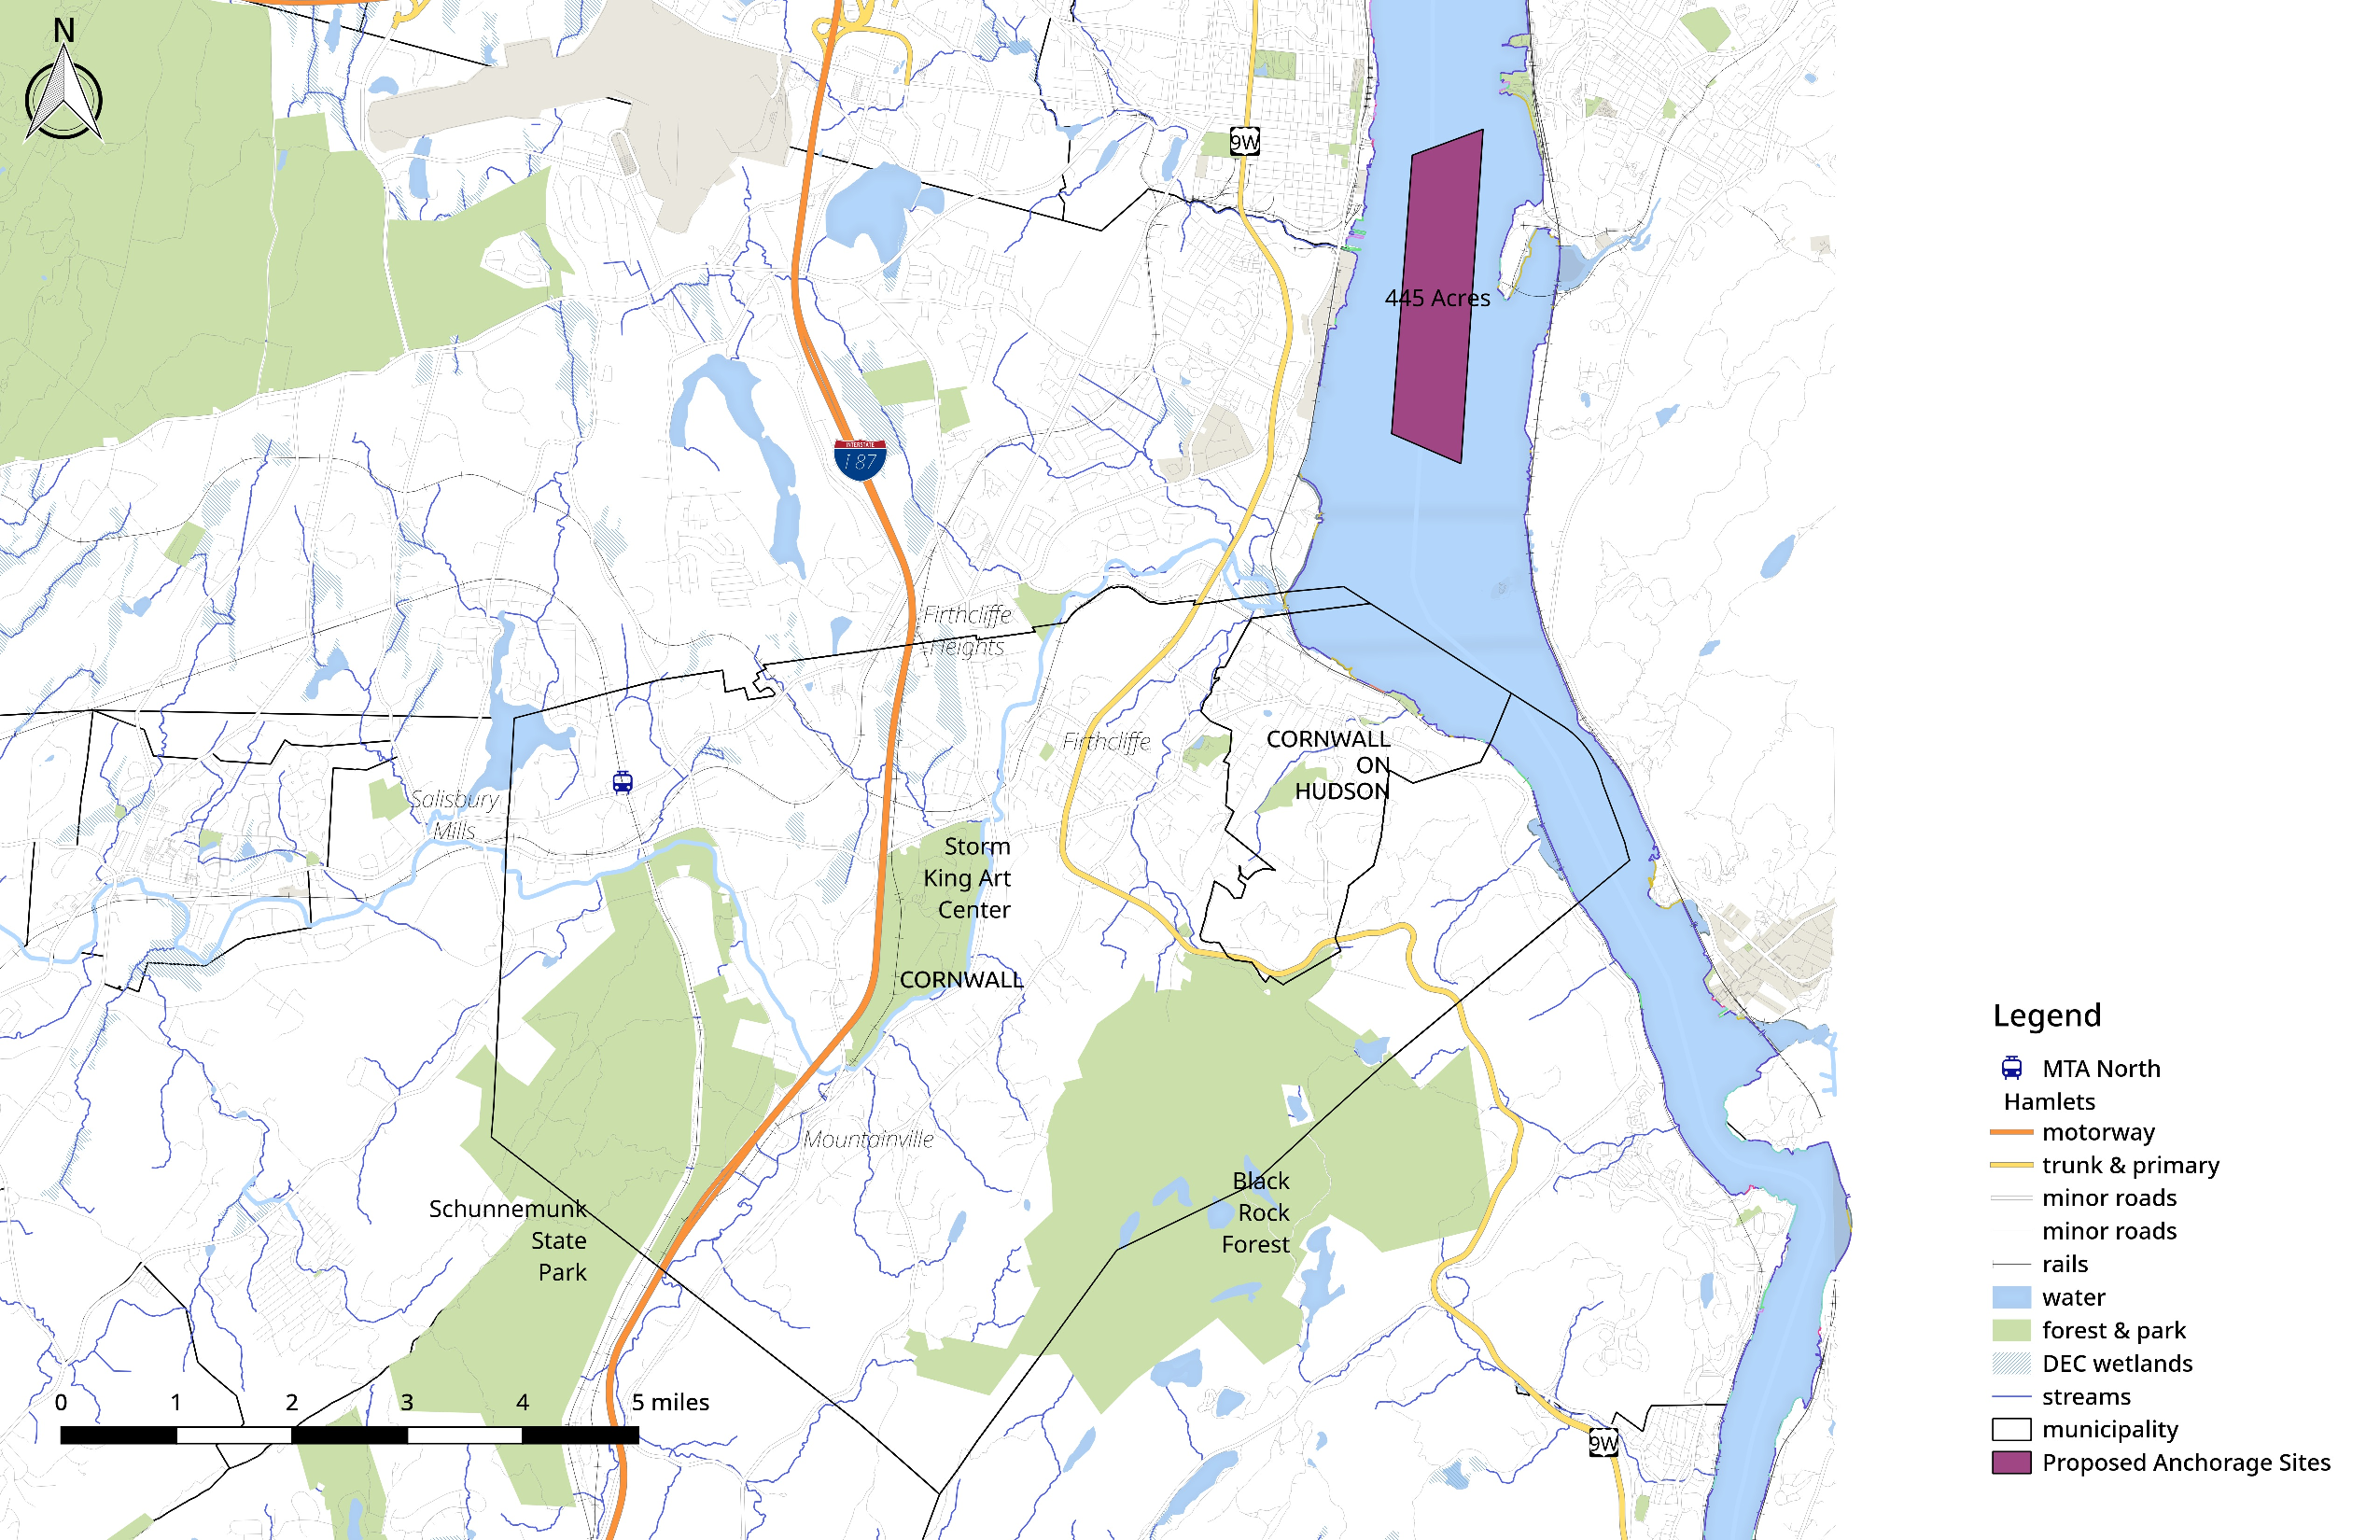
\includepdf[pages=-,fitpaper]{cornwall_maps/proposed_anchorages.pdf}\label{map:proposedanchorages}
This map displays two of the 42 long-term proposed anchorage sites on the Hudson 
River that was submitted by the The Maritime Association of the Port of New 
York/New Jersey to the US Coast Guard in January 2016. The lifting of the oil 
export ban has increased barge traffic on the Hudson River, increasing the risk 
of an accident. The Newburgh hub would have room for a total of 8 barges, with 
space for 5 barges being moored adjacent to the City of Newburgh and 3 moored 
north of the Newburgh/Beacon Bridge. The first area of anchorage sites would 
make 445.34 acres of the Hudson available to barges and the latter would make an 
additional 305 acres of the Hudson available. These barges most likely will 
transport oil and environmental groups have warned that besides the risk of 
spills and explosions that this will turn the Hudson River into a parking lot. 
Due to backlash from engaged citizens, the Coast Guard scrapped the proposal and 
convened a Ports and Waterway Safety Assessment (PAWSA). Multiple workshops were 
held to gain stakeholder insight and plan for a safe Hudson River. Furthermore, 
Governor Andrew Cuomo signed a bill in October, 2017 which gives the 
\gls{nysdec} authority to regulate oil barges on the Hudson River and instructs 
the agency to enact ''tanker avoid zones``.


%*********************LULC**********************
\chapter{Land Use}\label{sec:landuse}
\section{Land Use and Land Cover}\label{subsec:landuse}
\subsection*{Why You Need This Map}
The natural beauty of the Hudson Valley is a source of pride for its residents 
and is responsible for our strong tourism industry. Our challenge is to preserve 
the region’s remaining beauty while allowing for appropriate land uses that 
least impact the natural resources important to our health and the health of our 
biological communities.
\par
Smart land use decisions are more important than ever. Extreme weather events 
and drinking water pollution and availability have highlighted the effects of 
poor land use decisions. For example, the increase in impervious surfaces from 
development of structures, parking lots, and roads have made some communities 
more flood prone. The fragmentation of undeveloped areas by roads and 
development impedes wildlife movement and reduces habitat quality. Poorly 
placed developments, such as those sited too close to streams or on steeply 
sloped land, can result in declining stream health, degraded aquatic habitats, 
and lower water quality due to erosion and pollution. Even agricultural land 
uses can have detrimental effects in a watershed if poor management practices 
permit excess nutrients, sediment, and pathogens into waterways.
\par
Better land use decision-making must start with an understanding of our natural 
resources. By viewing land use and land cover data along with maps of streams, 
waterbodies, forest cover, wetlands and hydric soils, and other sensitive 
resources, communities can make better decisions for future growth. According to 
the Smart Growth Network, one of the principles of smart growth is to preserve 
open space, farmland, natural beauty, and critical environmental areas by 
directing new development to existing community centers. These rediscovered 
traditional planning principles from centuries past can reduce municipalities’ 
future infrastructure needs and costs, and foster more walkable communities that 
support commerce in community centers.
\par
Haeckel and Heady (2014) note that "land cover data sets\ldots should not be 
used for site planning and are not a viable substitute for on-the-ground 
knowledge and site visits\ldots" Satellite-derived land cover data do, however, 
allow planners, planning boards, elected officials, and developers to understand 
patterns of land use and to identify possible impacts of development proposals 
on the larger context of surrounding natural resources.

\subsection*{Orange County Context}
The National Oceanic Atmospheric Administration’s Coastal Change Analysis 
Program (C-CAP) Land Cover Atlas for Orange County reveals an increase in 
development and impervious surface area between 1996 and 2010: developed area 
increased by 14.23\% and impervious surface area 16.89\%. The majority of the 
increased development has been Low Intensity Developed (LID), which is 
typically comprised of single family housing, particularly in rural 
neighborhoods, but also includes all types of land uses. Forested and 
agricultural lands have lost the most land to development, with losses 
calculated at 6.06 square miles and 4.46 square miles, respectively. The chart 
below shows the percentages of total developed land and total impervious surface 
area in Orange County in 1996 and 2010.
\begin{table}[ht]
\begin{center}
    \begin{tabular}{| l | l | l |}
    \hline
    Land Cover Changes & 1996 & 2010 \\ \hline
    Percent Developed & 9.6\% & 10.97\% \\
    Percent Impervious Surface Area & 3.26\% & 3.81\% \\ \hline
    \end{tabular}
    \label{tab:lc_change}
    \caption{Land Cover Changes in Orange County between 1996 and 2010}
\end{center}
\end{table}

\subsection*{Land Cover Map}\
The Land Cover map shows natural land cover classes, such as forests and 
grasslands; semi-natural habitats, such as farmland, pastures, and managed 
woods; and developed land cover, which in the Town of Cornwall and the Village 
of Cornwall-on-Hudson can include residential, commercial, and institutional 
uses.
\par
The majority of land cover for the combined municipalities is forest (see 
Forests Map). Our communities are fortunate to be cradled by large, 
unfragmented forests in Storm King State Park and Black Rock Forest along the 
southeastern municipal boundary and in Schunnemunk State Park along the 
southwestern boundary. There is additional undeveloped land in the form of 
wetlands, cultivated cropland, and land planted for pasture/hay. Forested areas 
appear in shades of green.
\par
The map areas colored from pale pink to maroon represent the developed areas, 
with increasing percentages of imperviousness. Generally, the combined 
municipalities see development concentrations in the northeast areas in grid 
sections C2 and D2 as well as around Beaver Dam Lake straddling grid sections 
A1/A2 and B1/B2. Developed areas also follow the principal vehicular routes of 
Angola Road, Long Hill Road, Mineral Spring Road, Orrs Mill Road, Clove Road 
(aka County Road 27), State Route 94, State Route 32 (aka Woodbury Road), and 
Federal Highway 9W. The Village’s developed area is roughly a third of its total 
land cover. The Town’s developed area accounts for roughly one eighth of the 
total land cover.
\par
Cross referencing the Land Cover map with the Steep Slopes Map illustrates that 
development in the Town and Village is primarily located on slopes of less than 
15\%. Some development has occurred in the more wooded and steeper mountainous 
slopes between 15.1\% and 25\%. Future development on these slopes is 
discouraged due to the increased propensity for erosion and expensive drainage 
treatments that may not work for the long term. Additionally, building in the 
more mountainous areas results in loss of forest cover and wildlife habitat. 
Only in relatively few areas have the Town and the Village built on very steep 
slopes of greater than 25\%. Current zoning no longer allows for construction on 
very steep slopes.
\par
Agricultural production is present in Cornwall, represented on the map as 
cultivated crops, hay, and pasture and running along the central area of both 
municipalities. These areas appear as browns, greys, and yellows. Cornwall's 
agricultural areas are also some of the most scenically beautiful areas in our 
communities. 
\par
Woody and emergent herbaceous wetlands (slate blues) occur primarily in the 
lower elevations in the northern part of the Town and along waterways. They are 
not readily apparent on this map, but can be best identified when cross 
referencing the ~\nameref{map:wetlandsandhydricsoils}. More details on the distribution 
of wetlands in the municipalities are included in ~\nameref{subsec:wetland}.

\includepdf[pages=-,fitpaper]{cornwall_maps/LandCover.pdf}
~\label{map:landcover}
\section{Farmland}\label{subsec:farmland}
\subsection*{Why You Need This Map}
Agriculture is a significant part of the economy and character of the
communities in Orange County and New York State. The Hudson Valley in
particular has seen a boom in agro-tourism, breweries and distilleries, and
organic farming operations that feed urban demand for locally-sourced produce.
The definition of farmland in this chapter includes actively cultivated
cropland, livestock pastures, orchards, hayfields, and nurseries. Statewide,
there are more than 35,000 farms on approximately 7 million acres, which
represents more than 20\% of the state (NYS Agricultural Society). New York
ranks high among the major agricultural states in the nation, ranking in the
top 10\ in production of 30 commodities. It is the second largest producer of
apples, snap beans and maple syrup, third in cabbage, grapes and dairy, which
is largest segment of the State's agricultural sector, and fourth in pears (NYS
Dept. of Agriculture and Markets). Even so, farmland in New York is rapidly
diminishing in the face of increased residential development and the decline of
small family-owned farms. According to the American Farmland Trust:
\begin{itemize}
    \item More than 4,000 farms in New York State have been lost to real estate
    development since the 1980s.
    \item More than 80\% of the fruits and vegetables grown in New York come 
    from farms that are currently threatened by development
    \item 30\% of New York farmland is owned by farmers who are over the age of 
    65
    \item Only 5\% of farmland in New York has been permanently protected
\end{itemize}
Creating an inventory of these farm parcels is vital to prioritizing the most 
important agricultural areas in the Hudson Valley region for preservation, and 
encouraging new agricultural commerce on existing farmland.

Soil quality and characteristics are the foundation of the agricultural economy 
in New York, and soil features like nutrient load, acid/pH balance, the ability 
to hold or drain moisture, slope, and texture (grain size), are all important 
for agricultural productivity. These characteristics differ widely based on 
things like the underlying geology, glacial history and flooding frequency, and 
soils can sometimes be very different even in two fields that are in close 
proximity. Because of the importance of these soil qualities, soils are very 
specifically classified by the U.S. Department of Agriculture. The 
classifications are then grouped into larger designations that generally 
indicate how productive the soil could be for agriculture. The chapters on 
~\nameref{subsec:calcareous} and ~\nameref{subsec:bedrock} provide additional 
detail on this topic and these designations.
%Calcareous and Glacial Outwash Soil

\subsection*{Farmland Soils and Agricultural Parcels in the Town of Cornwall 
and the Village of Cornwall-on-Hudson}
If agriculture is important to the regional economy and the character of the 
Town, then it is important to know where farms are, and the location of soils 
that best lend themselves to farming. This map shows where various farm parcels 
are located within Cornwall’s borders, as well as where the best agricultural 
soils are located, as identified by the U.S. Department of Agriculture. 

Cornwall does not have an abundance of farm parcels. Much of what was once 
farmland has been developed for residential, commercial and municipal uses over 
the centuries. The majority of remaining farmland parcels are located in the 
western part of the town and are dedicated to field crops like hay and horse 
farming pastures. There are a number of vacant farm parcels that feature 
prominently on the Meadows, Grasslands, and Shrublands Map. Also visible on the 
map, are a single parcel classified as orchard located at Jones Farm, and a 
single parcel classified as livestock and products along Route 94. 

The shaded areas showing Prime Farmland, Prime Farmland If Drained, and Soils 
of Statewide Importance match the areas profiled on the General Soil Classes 
map. More detailed descriptions of these soils can be found in the General Soil 
Classes chapter and the glossary for this \gls{nri}.

\includepdf[pages=-,fitpaper]{cornwall_maps/FarmlandSoilsandAgParcels.pdf}\label{map:farmlandsoilsandagparcels}
\section{Conservation and Public Lands}\label{subsec:conservation}
\subsection*{Why You Need This Map}
Conservation and public lands are areas where the natural resources identified 
in this report are most likely to be protected from future development. By 
mapping our existing protected lands, we can see where we can be confident that 
these natural resources are secure. Perhaps more importantly, we can find the 
gaps where there are important natural resources that are not yet protected, 
and identify areas that should be prioritized by the community for future 
protection. Of particular importance are undeveloped areas that act as linkage 
zones between existing preserved lands. Linking and expanding these natural 
habitats can help sustain healthy wildlife populations and reduce the potential 
for isolated habitat islands that are created when natural areas become 
surrounded by development. 
\par
Our region is fortunate in that there are several large blocks of protected 
land including Storm King State Park, Black Rock Forest Preserve, and 
Schunnemunk Mountain State Park. Each of these protected areas consists of over 
1,500 acres that are rich in natural resources that will never be threatened by 
development. Much of this land was protected through the work of state agencies 
and non-profit organizations with a mission to conserve natural resources. There 
are numerous non-profit organizations that are active in the area, including 
Black Rock Forest Consortium, Hudson Highlands Land Trust, Open Space 
Institute, Orange County Land Trust, and Scenic Hudson, and the amount of 
protected land is likely to continue to grow through their work. 
\par
The categories of protected land shown on the maps included with this report 
have differing methods and levels of protection. Conservation easements are 
areas where the land is owned privately, but future development is restricted in 
order to protect the property’s conservation values. Municipal Parks may be 
protected with a primary goal of providing recreational opportunities to the 
community. There are also properties that are not shown on the map that are not 
formally protected, but function as conservation lands because they are owned by 
an entity that values natural resources such as an educational institution. 

\subsection*{Protected Open Space Map}\label{subsec:protectedopenspace}
The Town of Cornwall and Village of Cornwall-on-Hudson have significant areas of 
protected land. Together, these municipalities contain 7,473 acres1 of protected 
land, which represents approximately 38\% of the land in these municipalities. 
Approximately 21\% of the Village of Cornwall-on-Hudson is protected. 

The following is a description of the categories of protected land within the 
Town of Cornwall and Village of Cornwall-on-Hudson.

\paragraph{State Parks: 2,933 Acres}Storm King State Park and Schunnemunk State Park are partially located in the Town of Cornwall. These parks are managed by the Palisades Interstate Park Commission, and they are open to the public for passive recreation.

\paragraph{Nature Preserves: 2,024 Acres}
Black Rock Forest is the most significant protected area in the Town. Black 
Rock Forest consists of 3,643 acres, the majority of which are in Cornwall. The 
forest contains over 23 miles of trails that are open to the public for passive 
recreation. Black Rock Forest is also permanently protected by a conservation 
easement. 

Other nature preserves include the Leone Preserve, which is owned by the Orange 
County Land Trust, and the Hudson Highlands Nature Museum, which is also 
permanently protected by a conservation easement.

\paragraph{Conservation Easements: 987 acres}
There are 10 conservation easements in the Town and Village, which are held by 
various non-profits, including the Hudson Highlands Land Trust, Open Space 
Institute, Orange County Land Trust, and Scenic Hudson. 

\paragraph{Municipal Parks: 79 acres}
Municipal parks include Riverlight Park, Roe Park, and Harold Avenue Park 
(Laurel Crest Park) in the Town, and Donahue Memorial Park in the Village. Some 
of these parks are designed and developed for active recreation with ball 
fields and facilities (such as Riverlight Park), while others are largely 
undeveloped and open for passive recreation (such as Roe Park).

\includepdf[pages=-,fitpaper]{cornwall_maps/ProtectedOpenSpace.pdf}\label{map:protectedopenspace}
\section{Zoning and Tax Maps}\label{subsec:zoning}
\subsection*{Why You Need These Maps}
New York State's zoning enabling statutes state that comprehensive plans must 
provide for the "immediate and long-range protection, enhancement, growth, and 
development" of a locality, with land use regulations, including zoning, 
"conform[ing] to the locality's comprehensive plan" (Salomone 2004).1 All land 
use regulations are enacted to "promote the public health, safety, and general 
welfare;" "[z]oning is primarily enacted to control the use of land and the 
density of those uses"~\citep{haeckel2014}.  Local zoning can also impose 
greater restrictions than state law to protect, for example, natural areas and 
cultural resources, such as historic locales, scenic areas, groundwater, 
floodplains, wetlands, and wildlife habitats.

The following maps for the Town of Cornwall and Village of Cornwall-on-Hudson 
show the zoning districts, special overlays/districts, and tax parcels within 
our community. The narrative will focus primarily on considerations for 
additional protective measures for our natural resources as authorized by 
Municipal Home Rule Law (Salomone 2004). The natural resources found in each 
district are described in relationship to the permitted uses within each 
district in Appendix F – Natural Resources within Zoning Districts and Overlays 
for the Town of Cornwall and the Village of Cornwall-on-Hudson.

\subsection*{Zoning and Parcels}
The following sections will focus on recommendations for additional measures 
important to the immediate and long-range protection of our quality of life and 
natural resources. Some recommended protective measures are applicable to both 
the Town and Village. (Additional information regarding the recommended 
measures below can be found in Appendices C, H, I, and J.)2

\section{Town of Cornwall}
Zoning Chapter 158 of the Code of the Town of Cornwall describes the uses 
allowed in 12 zoning districts and 2 overlays. The tables of General Use 
Regulations provide an overview of the uses permitted by right, uses by special 
permit, and permitted accessory uses.
\begin{itemize}
    \item The Town should consider developing an aquifer protection overlay 
    district as well as a Source Water Protection Plan to protect the supply 
    and quality of drinking water.  Exclusion of bulk storage should be 
    considered.
    \item The Town should consider developing steep slope regulations that limit 
    construction on slopes exceeding 15\% to protect against erosion, 
    sedimentation of streams and down-slope areas, landslides, and the 
    degradation of scenic views.
    \item The Town should consider strengthening current language pertaining 
    to tree removal (see chapter 75 – Clearing and Grading) by developing tree 
    preservation legislation. Such legislation would enable the Town and its 
    residents to take advantage of the natural benefits that are intrinsic to 
    trees: 
    flooding control, filtration of pollutants and prevention of erosion, 
    protection of watershed areas, improvement of air quality, noise barriers, 
    habitat for wildlife, and cooler micro-climates.
    \item The Town’s zoning chapter 90, Freshwater Wetlands Protection Law, is 
    very comprehensive. The Town should consider improving the Law by supporting 
    the identification of wetlands as small as half an acre and applying the 
    existing Law to this wetland size.3 (Half an acre of wetland can store up 
    to three-quarters million gallons of floodwater at no cost to a 
    municipality.) The identification of smaller wetlands can be done as a 
    citizen science project in partnership with the Cornwall Conservation 
    Advisory Council, the Cornwall Central School District, and community 
    residents.4 Additionally, the Town should explore providing adequate 
    protection for inter-jurisdictional wetlands by working to develop equally 
    protective regulations with adjoining municipalities.
    \item Throughout the Town’s Code, the presence of a wetland can result in 
    the denial of a permit for clearing and grading and/or building within a 
    100-foot buffer. However, no such language exists for streams. The Town 
    should consider developing a Stream Buffer Overlay for perennial and 
    seasonal waterways in order to maintain water quality, recharging of 
    groundwater, waterway health for wildlife, and bank stabilization and 
    erosion control. A minimum buffer of 200 feet is recommended; wider buffers 
    should be considered for habitat protection of specific wildlife (see 
    Strong, 2008). Orange County has developed a model riparian buffer local 
    law.
    \item The Town’s Code includes language referencing the minimization of 
    public and private losses from flood conditions by controlling the 
    alteration of natural floodplains and their associated stream channels 
    and natural protective barriers.  The Town should consider developing a 
    Floodplain Overlay District to clearly outline areas to be protected 
    and, given the increase in severe storms, also consider protections to 
    the five-hundred-year floodplain.
    \item The Town should consider referencing green infrastructure practices 
    as part of Code Chapter 121 on Stormwater Management.
    \item The Town should consider expanding the application of Conservation 
    Subdivision Design Layout to all districts currently zoned MCR and ARR as 
    well as increasing the minimum percentage of open space to 80\%. The 
    positive resulting impact from these changes would include less expensive 
    construction costs, less clearing and grading, and preservation of the 
    visual and environmental integrity of most of the landscape (OCWA 2014).
    \item The Town should consider tasking the Cornwall Conservation Advisory 
    Council with the development of a comprehensive listing of native plantings 
    to support the intent of the Ridge Preservation Overlay District. 
    Additionally, a listing of said planting can be made available to 
    developers, residents, and businesses to further enhance the beauty of our 
    Town without inviting nuisance plant species. (See Village recommendation 
    for additional detail.)
\end{itemize}

\includepdf[pages=-,fitpaper]{cornwall_maps/TownZoning.pdf}
\label{map:townzoning}
%{Zoning and Parcels Map}

\section{Village of Cornwall-on-Hudson}
Zoning Chapter 172 of the Code of the Village of Cornwall-on-Hudson describes 
the uses allowed in 6 zoning districts and 2 overlays.
\begin{itemize}
    \item The Village should consider managing stormwater by limiting 
    impervious coverage through maximum development coverage areas rather than 
    maximum lot coverage percentages. The former limits the portion of a lot 
    covered by buildings, parking areas, accessory structures, and other 
    impervious materials.
    \item The Conservation Residential CR-3 District (scenic) provides for a 
    conservation green belt setback of 25 feet along both sides of Deer Hill 
    Road where no tree cutting, construction, or other development is 
    permitted. The Village should consider adding language to encourage 
    bringing properties into conformance.
    \item The Village should consider incorporating language that encourages the 
    use of native plantings suitable for hardiness zone 6. NYSDEC’s Division of 
    Lands and Forests provides many native suggestions for flowers; grasses, 
    ferns, groundcovers; shrubs; trees; and vines.
    \item The Industrial District’s currently permitted uses may be negatively 
    impacted by projected sea level rise. The Village should consider 
    additional limitations on industrial uses or additional precautionary 
    measures of currently permitted uses that may negatively impact the 
    aquifer, wetlands, and floodplains present.
    \item The Village should consider referencing green infrastructure 
    practices as part of Code Chapter 132 on Stormwater Management and for 
    off-street parking for 10 or more vehicles.
    \item The Village should consider developing a Floodplain Overlay District 
    to clearly outline areas to be protected and, given the increase in severe 
    storms, also consider protections to the five-hundred-year floodplain.
    \item The Village should consider developing a Wetlands and Watercourses 
    Overlay with a minimum buffer of 200 feet for surface waters of the State of 
    New York.
    \item The Village should consider a minor amendment to Chapter 151 Trees, 
    Shrubs, and Bushes to increase successful plantings of trees on private 
    properties: burlap should be removed prior to planting.
\end{itemize}
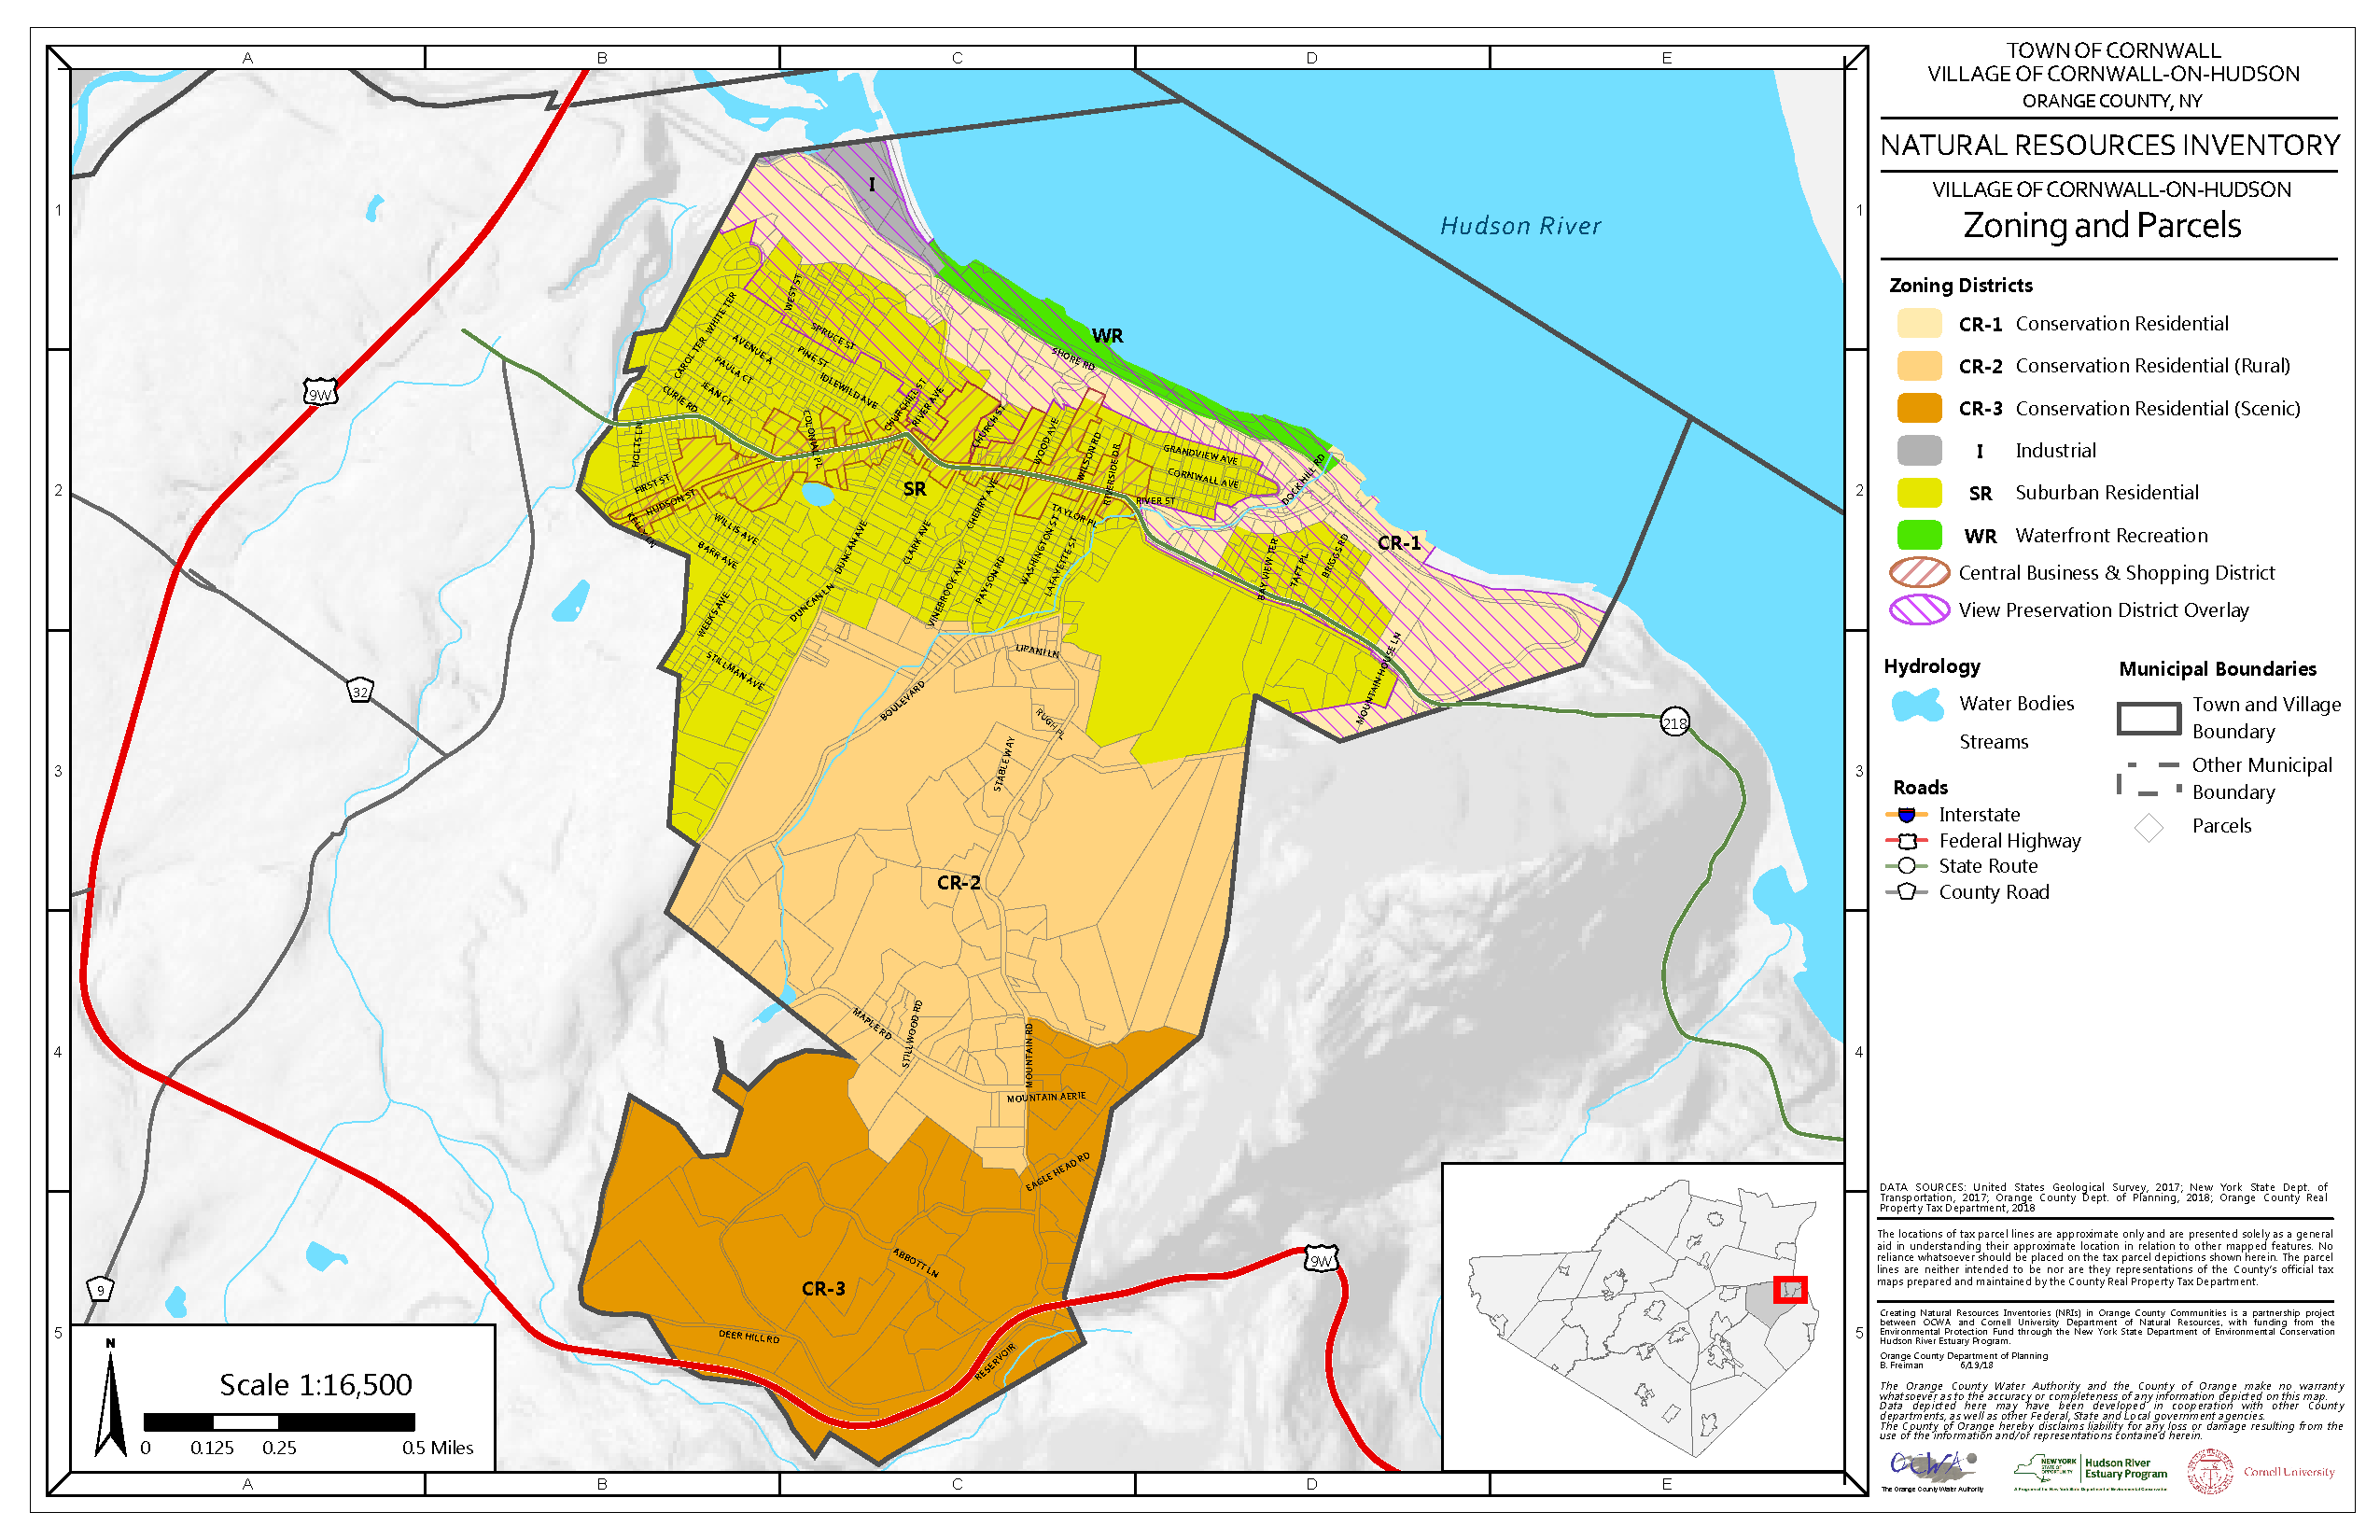
\includepdf[pages=-,fitpaper]{cornwall_maps/VillageZoning.pdf}\label{map:villagezoning}

%\subchapter{Figures}
%There will be some figures here maybe.

%\part{References, Appendices \& Glossary}
%**************References**********************
\chapter{References \& Resources}
\label{sec:references}
\printbibliography

%Glossary%%%%%%%%%%%%%%%%%%%%%%%%%%%%%%%%%%%%%%%
\chapter{Glossary and Acronyms}\label{subsec:glossary}
\glsaddall
\renewcommand{\glossarysection}[2][]{}
\printglossary

%\addtocounter{subchapter}{1}
\chapter{Known Species of Conservation Concern}
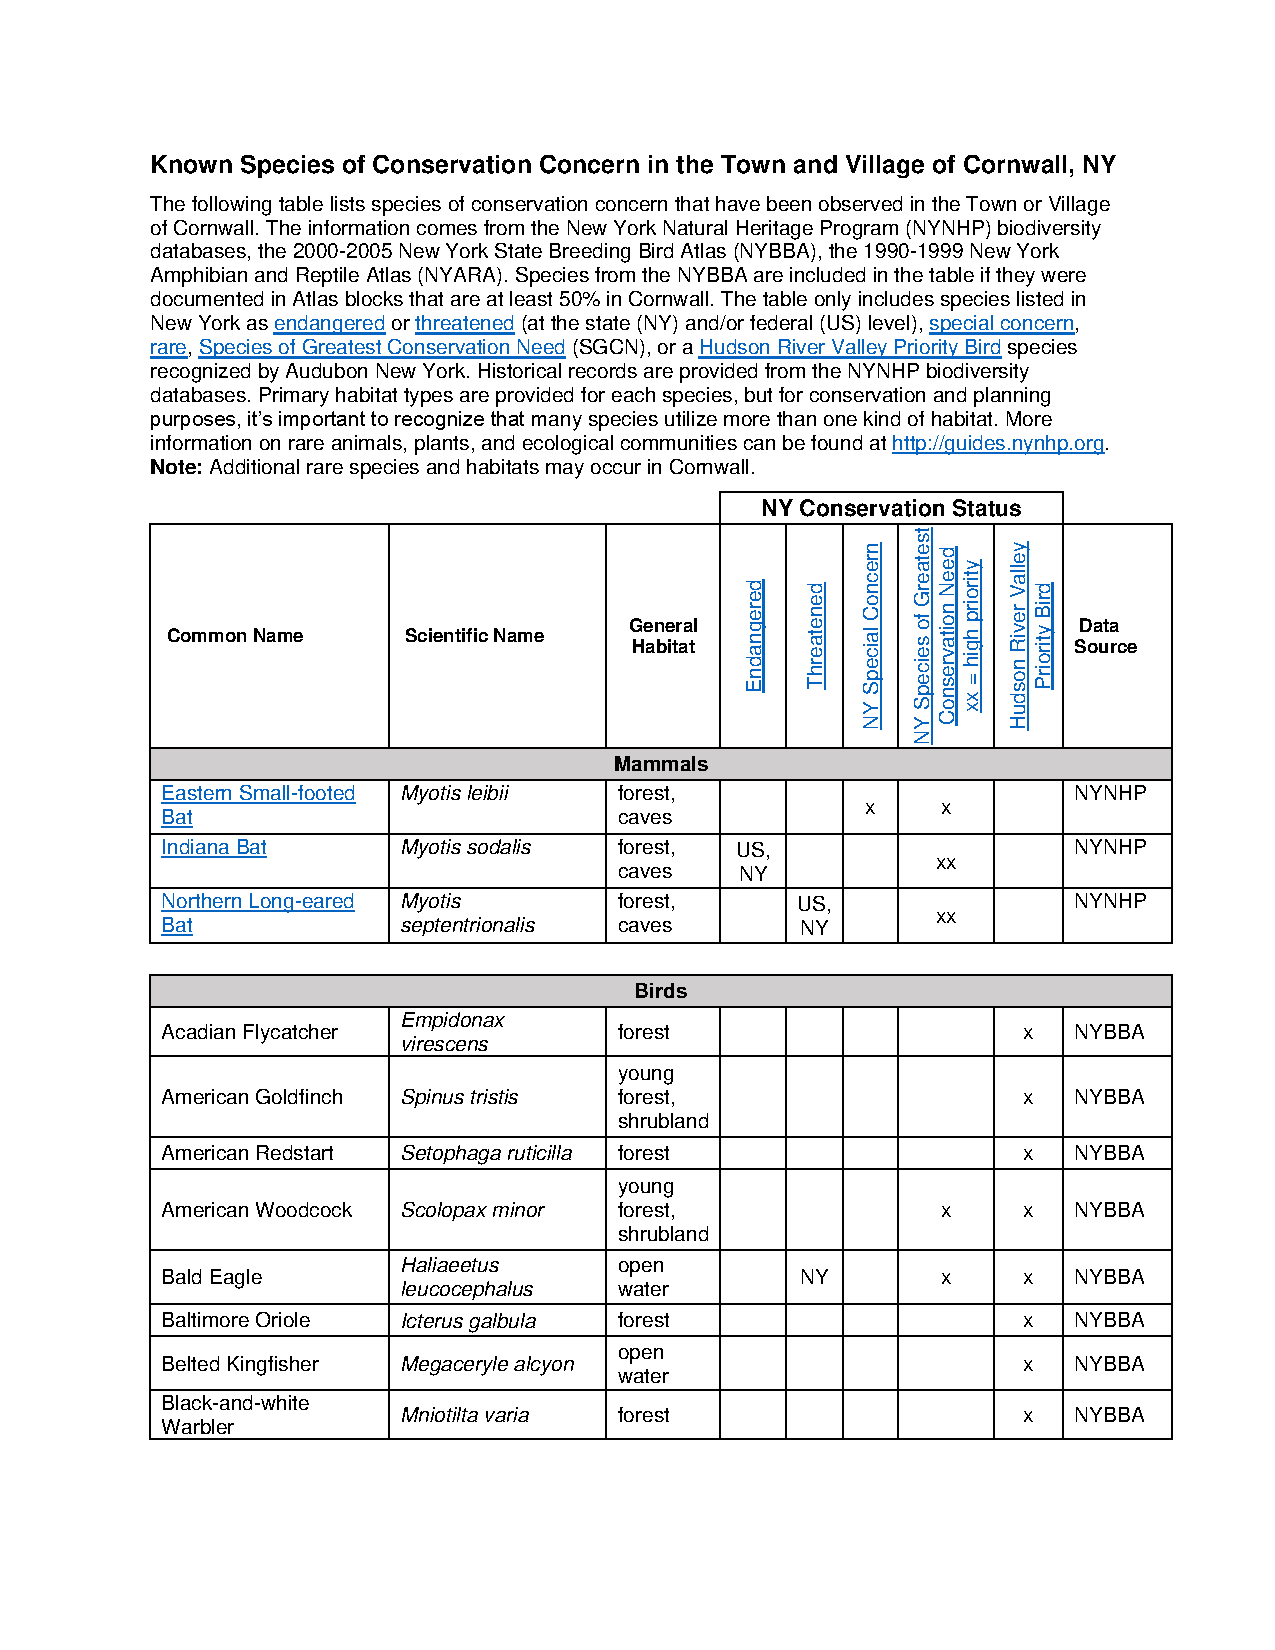
\includepdf[pages=-]{appendix/cornwall_B.pdf}
\namedlabel{app:cornwallspecies}{Known Species of Conservation Concern in the 
Town of Cornwall and Village of Cornwall-on-Hudson, NY}

%\addtocounter{subchapter}{1}
%\addcontentsline{toc}{subchapter}{\Alph{subchapter} \hspace{4mm}
\chapter{Summary of Municipal Wetland and Watercourse Protection Techniques}
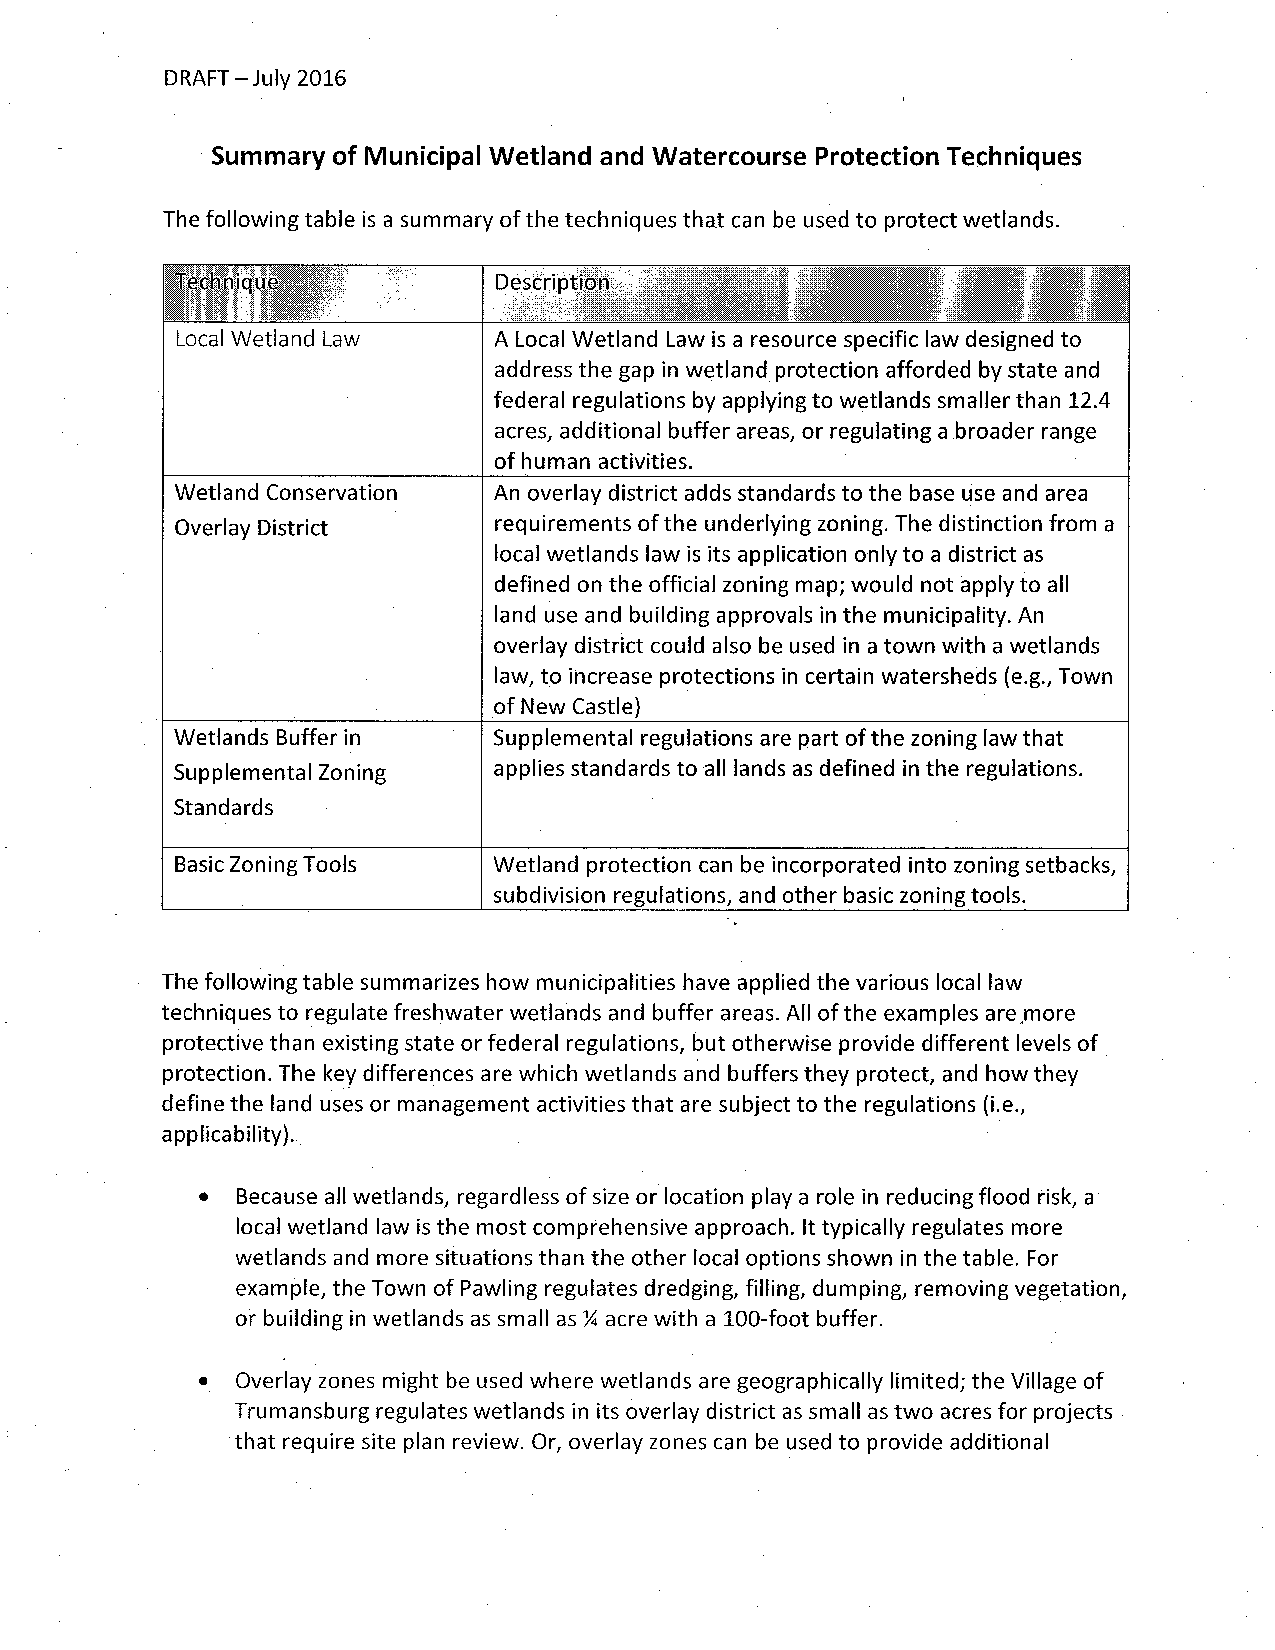
\includepdf[pages=-]{appendix/cornwall_C.pdf}\label{app:wetland_protection}

\chapter{National Wetland Inventory Wetland Classes}
\begin{table}[h]
    \centering
    \begin{tabular}{l l l c c }
    Municipality & Name & Acres & Percentage \\
    \hline
    \multirow{7}{*}{Town of Cornwall}
    & Estuarine \& Marine Deepwater & 296 & 41\%  &\\
    & Freshwater Forested/Shrub Wetland & 171  & 24\%  &\\
    & Freshwater Pond & 107 & 15\% &\\
    & Freshwater Emergent Wetland & 71 & 10\% & \\
   	& Lake & 56 & 8\% &\\ 
    & Riverine & 20 & 3\% &\\
    & Total & 721 & 100\% &\\
    \hline
    \multirow{5}{*}{Village of Cornwall-on-Hudson}
    & Estuarine \& Marine Deepwater & 390 & 98\%  &\\
    & Freshwater Pond & 3 & 0.8\% &\\
    & Freshwater Emergent Wetland & 2 & 0.5\% & \\
    & Riverine & 1 & 0.3\% &\\
    & Total & 396 & 100\% &\\
    \end{tabular}
    \caption{\gls{nwi} percentages per municipality}
    \label{tab:cornwall_nwi}
\end{table}

\label{app:cornwall_wetlands}

\chapter{Additional Information on Climate Conditions and Projections}
\includepdf[pages=-]{appendix/cornwall_E.pdf}\label{app:climate_projection}

\chapter{Natural Resources within Zoning Districts and Overlays}
%for the Town of Cornwall and the Village of Cornwall-on-Hudson}
This Appendix refers to the Zoning and Parcels Maps for the Town of Cornwall and the Village of Cornwall-on-Hudson. Brief descriptions of permitted uses within each district as well as the natural resources contained therein are bulleted below.

Town of Cornwall
\begin{itemize}
    \item Generally, the majority of districts allow varying levels of residential development.
    \item The Agricultural Rural Residence District permits uses related to agriculture, uses generally appropriate for large open spaces, and single-family detached homes.
    \begin{itemize}
        \item The ARR district is underlain by aquifers in the flatter lands around Schunnemunk Mountain (see A2/A3/B2/B3 in this map and in Public Wells, Aquifers, and Risk Sites Map).
        \item Steep slopes are found at the base of Schunnemunk Mountain (see A3/B3 and in the Steep Slopes Map), between Long Hill Drive and Mineral Springs Road (C4 in the Steep Slopes Map), and at the base of Black Rock Forest (C4 in the Steep Slopes Map).
        \item Along Cornwall’s southeastern border, stepping stone, locally significant, and regionally significant forests are part of this district.
        \item Federally and state designated wetlands are found in this district. Also present are hydric soils, which are probable wetlands. (See grid boxes A2/A3, B2, C4, D2; also see same grid boxes in Wetlands and Hydric Soils Map.)
    \end{itemize}
    \item The Local Shopping District permits a variety of uses, including gasoline service facilities by special permit and uses accessory to motor vehicle repair shops and used vehicle sales.
        \item Of the 3 areas where these districts are found, only the district in Mountainville, where Pleasant Hill Road and state route 32 intersect, presents a concern as this area is underlain by an aquifer, is adjacent to Class C trout spawning stream, and falls within a 100-year and 500-year floodplain.
    \item No concerns for uses permitted in the General Commercial Shopping District are identified as related to the Town’s natural resources.
    \item The Highway Commercial District permits uses ranging from small-scale to large-scale commercial development, including automobile repair facilities, undertaking and funeral establishments, parking lots and parking facilities, large retail facilities, and gasoline service facilities.  Use groups A thru J allow for high maximum development coverage, resulting is a large portion of impervious coverage.
    \begin{itemize}
        \item The District located along federal highway 9W northeast of Willow Avenue is located within a stepping stone forest and regional forest linkage zone.
        \item The District located on state route 32 near the Town of New Windsor boarder is underlain by an aquifer, falls within a regional forest linkage zone, and is adjacent to or within federally and state designated wetlands.
        \end{itemize}
    \item The Mountain and Conservation Residence District permits appropriate uses with low maximum development coverage.  Of the five areas zoned MCR, four fall entirely or partially within protected open space.
    \begin{itemize}
        \item The area bounded by Orrs Mills Road, state route 32, Pleasant Hill Road, and interstate 87 (B2/B3 \& C2/C3) is underlain by aquifers, contains wetlands of federal and state importance and hydric soils, has steep slopes in excess of 15\%, has a Class C stream supporting trout, prime farmland soil, and is a regional forest linkage zone with stepping stone forest.
        \item The area west of interstate 87 and north of the Schunnemunk State Park boundary has regionally significant forest, some prime farmland, and a Class C stream supporting trout.
        \end{itemize}
    \item The Mixed Residence District permits a variety of uses, including single-family dwellings, multiple dwelling development, and clustered higher density residential development (two-family detached, townhouses, row). Use groups C and D permit high maximum development coverage.
    \begin{itemize}
        \item The MR area in B1/B2, which is largely occupied by Cornwall Central High School, is underlain by aquifers, contains hydric soils and federally and state designated wetlands, a Class C stream supporting trout, and contains stepping stone forest within the regional forest linkage zone.
        \item The MR area in A2 contains hydric soils and federally designated wetlands as well as stepping stone forest within the regional forest linkage zone.
        \end{itemize}
    \item The Planned Commercial District permits many uses, including laboratories and related offices, light manufacturing, industrial parks, printing plants, and general manufacturing and industrial processing operations. These uses are allowed a high maximum development coverage.  The PCD areas below are identified by the map grids in which they fall.
    \begin{itemize}
        \item The area in D1, occupied by New York Military Academy, is adjacent to Idlewild Creek—a Class C stream supporting trout.
        \item The area in C1/C2 is the former site of the Firthcliffe Carpet Mill Company and Majestic Weaving, and current site of a number of small businesses. This area is adjacent to the Moodna Creek, a 100-year floodplain Class C stream supporting trout. It is currently designated a DEC remediation site and contains stepping stone forest within the regional forest linkage zone.
        \item The area in B3, occupied by Tectonic Engineering \& Surveying Consultants, is underlain by an aquifer but has a relatively small percentage of impervious coverage.
        \item The area in B4 is completely underlain by an aquifer; includes the Woodbury Creek’s, a Class C trout spawning stream, 100- and 500-year floodplain; a federal wetland and hydric soils; prime farmland soils; and stepping stone forest.  The majority of this area is protected by a conservation easement.
        \end{itemize}
    \item The Planned Industrial/Office District permits many uses, including laboratories and related offices, light manufacturing, industrial parks, printing plant, outdoor storage of painting supplies, raw materials, fuels; general manufacturing and industrial processing operations; and above ground storage of crude oil and volatile products.  Use groups A thru G are allowed a high maximum development coverage.  The PIO areas below are identified by the map grid sections in which they fall.
    \begin{itemize}
        \item The area in D1 is underlain by an aquifer; includes the Moodna Creek’s, a Class C trout spawning stream, 100-year floodplain and a federal wetland.
        \item The area in B1/C1 is almost entirely underlain by an aquifer; contains federally and state designated wetlands, and contains stepping stone forest within the regional forest linkage zone.  Review of the Google Maps satellite image appears to show a sufficient buffer between the existing construction and adjacent wetlands. Development along Hollaran Road does not follow cluster development principles.
        \item The area in B4 is underlain by an aquifer; includes the Woodbury Creek’s, a Class C trout spawning stream, 100- and 500-year floodplain; contains hydric soils; prime farmland soil; and stepping stone forest.
        \end{itemize}
    \item The Planned Residential District permits limited uses. This area in C1 is peppered with federal wetlands and contains stepping stone forest within the regional forest linkage zone. Conventional suburban development abuts the southwestern portion of this pristine patch of forest.
    \item The Suburban Low-Density Residence District permits a variety of uses, including single-family dwellings.
    \begin{itemize}
        \item The area on both sides of Angola Road has a federal aquifer and hydric soils on the northern end, three Class C streams supporting trout, steep slopes in excess of 15\%, and contains stepping stone and regionally significant forests.
        \item The area north of Orrs Mills Road and west of interstate 87 is underlain by a large aquifer, has a number of federally and state designated wetlands and hydric soils, two Class C streams supporting trout, and stepping stone forest in a regional forest linkage zone.
        \end{itemize}
    \item The Suburban Residence 1 District permits uses related to outdoor recreation, agriculture, institutional, and low to medium density housing.
    \begin{itemize}
        \item The area around Beaverdam Lake contains federal wetlands and hydric soils, a Class C stream supporting trout, and stepping stone forest in a regional forest linkage zone.
        \item The area from B1/B2 to D1/D2 contains a number of federal and state wetlands and hydric soils, a number of Class C streams and Idlewild Creek—a Class C trout spawning stream, stepping stone forest in a regional forest linkage zone, and locally significant forest.
        \end{itemize}
    \item The Suburban Residence 2 District permits uses largely related to small professional offices and low to medium density housing. The area in C2/D2 contains a Class C streams and Idlewild Creek—a Class C trout spawning stream, some prime farmland, and a small portion falls within a 500-year floodplain. Use groups D, G, H, and I have high maximum development coverage. 
    \item The Schunnemunk Agricultural Scenic Overlay is located west of interstate 87 and south of Moodna Creek and Orrs Mills Road. Clustered subdivision layout can be required by the Planning Board through a Conservation Subdivision Design Layout, with a minimum open space allocation of 50\%.  The Overlay terms slopes in excess of 30\% as a significant barrier to development.  Areas of 50-100 feet buffer waterbodies, waterways, and wetlands from development.
    \begin{itemize}
        \item Within the Overlay is found 100- and 500-year floodplains, federal and state wetlands and hydric soils, aquifers, prime farmland, steep slopes in excess of 15\%, and regionally significant forest within a regional forest linkage zone.
        \end{itemize}
    \item The Ridge Preservation Overlay is designed to protect the visual and aesthetic resources of the Schunnemunk Mountains and Hudson Highlands ridgelines. Planning Board review includes consideration of plantings of “appropriate native deciduous and/or evergreen vegetation.”
\end{itemize}
Village of Cornwall-on-Hudson
\begin{itemize}
    \item Conservation Residential Districts 1-3 and Suburban Residential District permit single-family cluster development, which was authorized, among other intents, “to preserve the natural and scenic qualities of open space and to protect local ecology, major stands of trees, steep slopes, geological features, and other areas of environmental value” through the flexibility in design and development of land.
    \item The Conservation Residential CR-1 District permits residential, recreational, and riverine uses, with a maximum permitted lot coverage pf 15\%.
    \begin{itemize}
        \item The district is partially underlain by an aquifer and contains a Class C streams supporting trout.
        \end{itemize}
    \item The Conservation Residential CR-2 District (rural) permits residential uses as well as uses compatible with residential and small scale agricultural development, with a maximum permitted lot coverage pf 10\%. 
    \begin{itemize}
        \item The district contains hydric soils and federally designated wetlands, a significant area of very steep slopes in excess of 25\%, and is almost entirely covered by locally significant forest.
        \end{itemize}
    \item The Conservation Residential CR-3 District (scenic) permits residential uses as well as uses compatible with residential development, with a maximum permitted lot coverage of 10\%.  The district includes a conservation green belt setback of 25 feet along both sides of Deer Hill Road where no tree cutting, construction, or other development is permitted.  No criteria for bringing properties into conformance is identified.
    \begin{itemize}
        \item The district contains a Class C stream supporting trout and is covered by locally significant forest.
    \end{itemize}
    \item The Industrial District permits uses such as laboratory, manufacturing, printing, and high-density housing.
    \begin{itemize}
        \item This district is underlain by an aquifer, contains a few federally designated wetlands, is located entirely on a 100-year floodplain, and includes steep and very steep slopes on the southwestern edge of the district. By 2100, a 3-foot sea level rise would inundate over half of the district and a 6-foot rise would result in the inundation the entire area.
        \end{itemize}
    \item The Suburban Residential District permits a variety of uses, including residential, recreational, and instructional.
    \begin{itemize}
        \item The district contains areas within the 100- and 500-year floodplains, a Class C stream supporting trout, locally significant forest, and prime farmland soil. The district contains 5 petroleum bulk storage facilities on Hudson Street and state route 218, one of which is located on a portion of route 218 that flooded during Hurricane Irene.
        \end{itemize}
    \item The Waterfront Recreation District permits riverine uses. The district is entirely underlain by an aquifer and includes an existing petroleum bulk storage facility, contains numerous federally designated wetlands, falls within a 100- and 500-year floodplain, includes prime farmland, and contains a Class C stream supporting trout. By 2100, a 3-foot sea level rise would inundate over half of the district and a 6-foot rise would inundate the entire area.
   \item The Central Business \& Shopping District includes Hudson Street up to River Street as well as streets on either side of Hudson and permits largely standard commercial uses. Any natural resources related to this district are mentioned in the SR District section above.
    \item The View Preservation District Overlay encompasses districts north of Hudson Street and state route 218. The overlay provides for the preservation and protection of Hudson River views from existing public roads, parks, or legally accessible public property under the Village’s Scenic Resources Protection Law. The Law declares the protection of these views for present and future generations in the broader public interest. The District Overlay ensures that use and development on private lands of structures and natural plantings do not impact the views from public areas. Any natural resources related to this district are mentioned in the SR, CR-1, I, and WR district sections above.
\end{itemize}\label{app:zoning}

%\addtocounter{subchapter}{1}
%\addcontentsline{toc}{subchapter}{\Alph{subchapter} \hspace{4mm}
\chapter{Orange County Municipality Resiliency Code Audit}
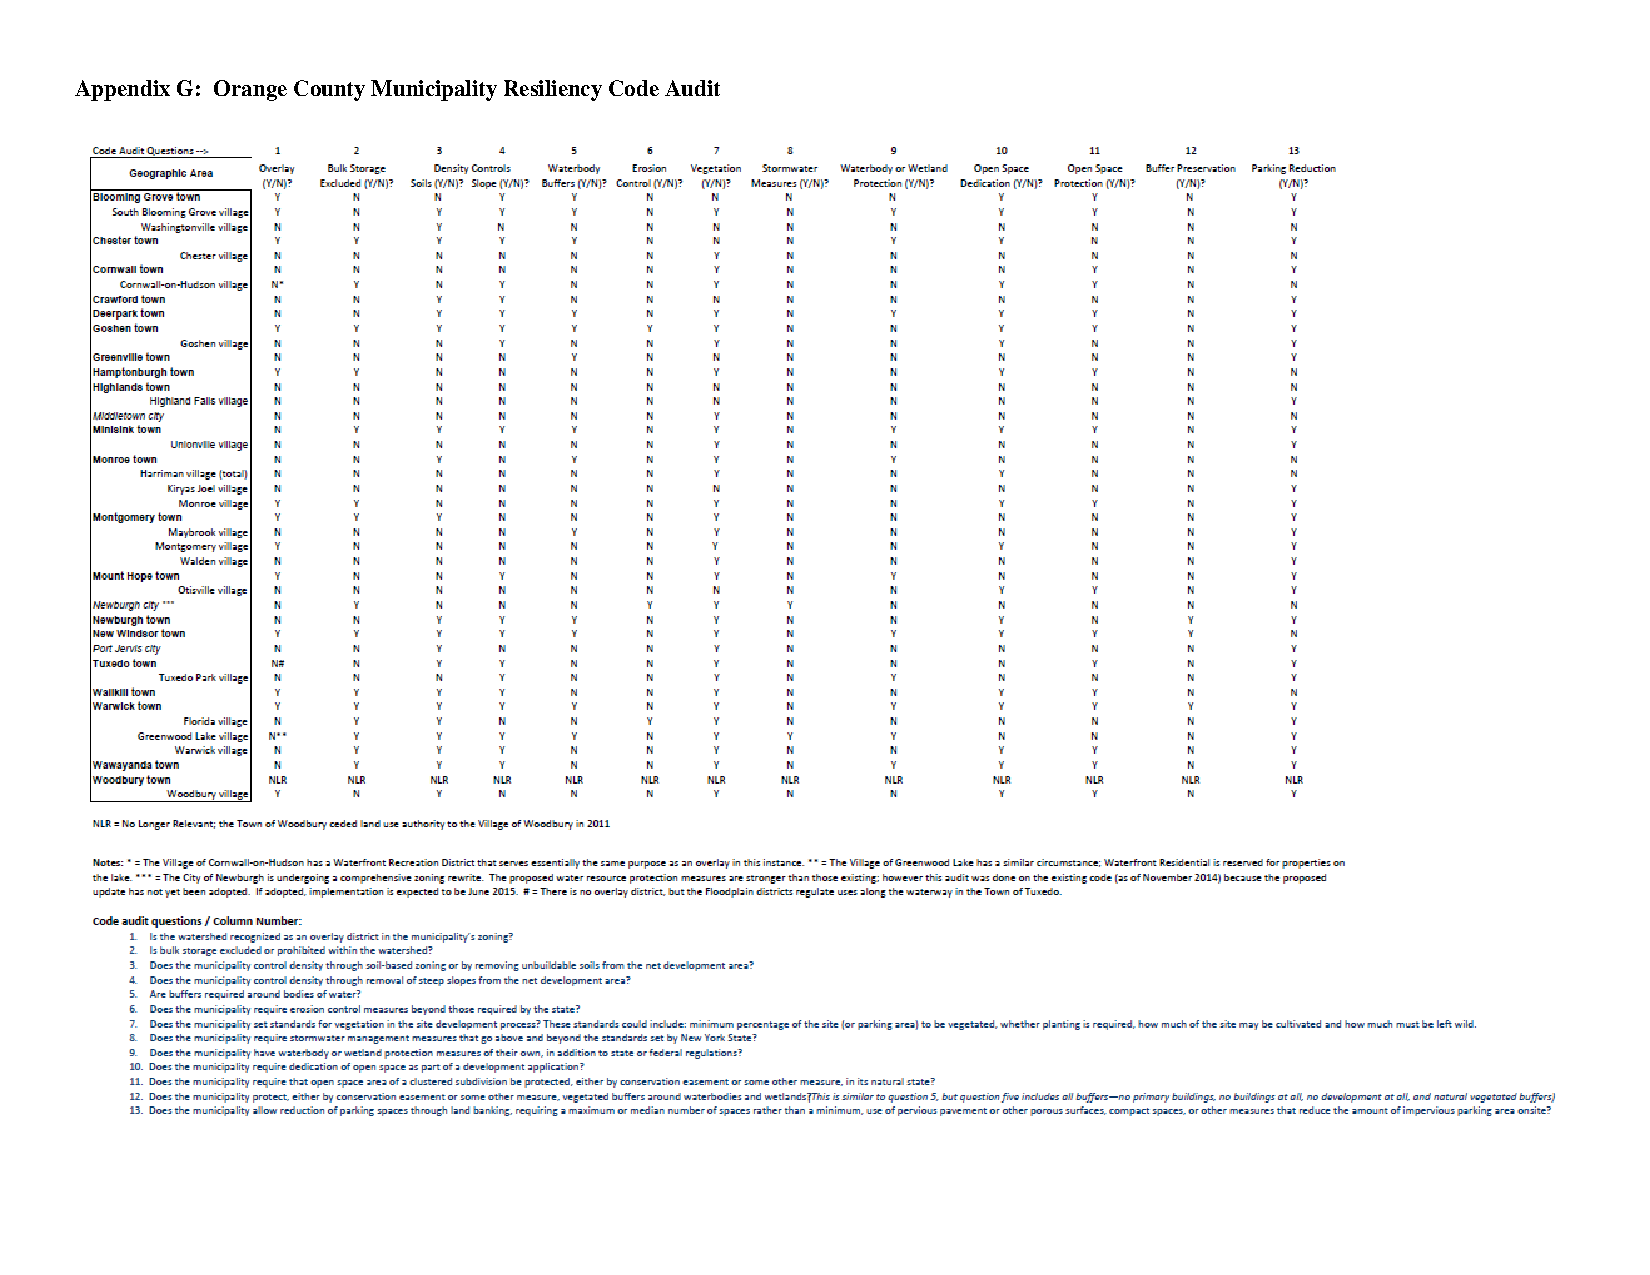
\includepdf[pages=-]{appendix/cornwall_G.pdf}\label{app:oc_resiliency}

%\addtocounter{subchapter}{1}
%\addcontentsline{toc}{subchapter}{\Alph{subchapter} \hspace{4mm}
\chapter{Water Quality \& Quantity Protection}
% from Pace Law School Land Use Law Center}
\includepdf[pages=-]{appendix/cornwall_H.pdf}\label{app:water_quality}


%\addtocounter{subchapter}{1}
%\addcontentsline{toc}{subchapter}{\Alph{subchapter} \hspace{4mm}
\chapter{Preservation of Natural Features}
%from Pace Law School Land Use Law Center}
\includepdf[pages=-]{appendix/cornwall_I.pdf}\label{app:pres_natfeatures}

%\addtocounter{subchapter}{1}
%\addcontentsline{toc}{subchapter}{\Alph{subchapter} \hspace{4mm}
\chapter{Compact Development \& Infill}
%from Pace Law School Land Use Law Center} 
\includepdf[pages=-]{appendix/cornwall_J.pdf}\label{app:compact_development}

%\noindent Some text here that is not indented...

%-------------------------------------------------------------------------------

%	INDEX
%-------------------------------------------------------------------------------

\cleardoublepage
\phantomsection
\setlength{\columnsep}{0.75cm}
\addcontentsline{toc}{chapter}{\textcolor{nriBlue}{Index}}
\printindex

%----------------------------------------------------------------------------------------

\end{document}